\documentclass{beamer}

\usepackage[utf8x]{inputenc}
\usepackage{graphicx}
\usepackage{amsthm,amssymb,amsbsy,amsmath,amsfonts,amssymb,amscd}
\usepackage{tikz}
\usepackage{dsfont}
\usepackage{array}
\newcolumntype{N}{@{}m{2pt}@{}}
\useoutertheme[subsection=false]{miniframes}
\usepackage{lmodern}

\setbeamercolor{author in head/foot}{fg=gray,bg=white}
\setbeamercolor{title in head/foot}{fg=gray,bg=white}
\setbeamercolor{page number in head/foot}{fg=gray,bg=white}
\setbeamercolor{section in head/foot}{bg=black,fg=gray}
\setbeamercolor{subsection in head/foot}{bg=black,fg=gray}

%%%%%%%%%%%%%%%%%%%%%%%%
% GENERAL BEAMER STYLE :

\setbeamertemplate{footline}{
  \hbox{%
    \begin{beamercolorbox}[wd=.2\paperwidth,ht=2ex,dp=1ex,left]{author in head/foot}%
      \hskip1em\usebeamerfont{author in head/foot}\insertshortauthor
    \end{beamercolorbox}%
    \begin{beamercolorbox}[wd=.7\paperwidth,ht=2ex,dp=1ex,center]{title in head/foot}%
      \usebeamerfont{title in head/foot}\insertshorttitle
    \end{beamercolorbox}%
    \begin{beamercolorbox}[wd=.1\paperwidth,ht=2ex,dp=1ex,right]{page number in head/foot}%
      \usebeamerfont{page number in head/foot}\insertframenumber{} / \inserttotalframenumber
      \kern1em 
    \end{beamercolorbox}
  }
}

\setbeamercolor{alerted text}{fg=red!80!black}
\setbeamercolor{itemize/enumerate subbody}{fg=gray!70!black}
\setbeamertemplate{itemize item}[square]
\setbeamertemplate{itemize subitem}[triangle]%{{\textendash}}
\setbeamerfont{itemize/enumerate subbody}{size=\footnotesize}
\setbeamerfont{itemize/enumerate subitem}{size=\footnotesize}

\setbeamertemplate{navigation symbols}{}

\AtBeginSection{
\begin{frame}
    \begin{centering}
    \begin{beamercolorbox}[sep=12pt,center]{part title}
    \usebeamerfont{section title}\insertsection\par
    \end{beamercolorbox}
    \end{centering}
\end{frame}
}



\title[Introduction to Gaussian Process Surrogates Models]{ \small MDIS Fall School 2017\\ \vspace{3mm} \Large Introduction to Gaussian Process Surrogate models}
\institute{Nicolas Durrande, PROWLER.io (nicolas@prowler.io) \\ Rodolphe Le Riche, CNRS LIMOS -- Mines St-\'Etienne (leriche@emse.fr)}
\author[MDIS 2017]{Clermont-Ferrand, Besse-en-Chandesse, 16th of October 2017}
\date{\null}

\DeclareMathOperator*{\Var}{var}
\DeclareMathOperator*{\E}{E}
\DeclareMathOperator*{\Cov}{cov}
\newcommand\PR[1]{\mathrm{P}\left(#1 \right)}
\newcommand\PS[1]{{\langle #1 \rangle}_\mathcal{H}}
\newcommand\PSi[2]{{ \left \langle #1 \right \rangle}_{\! #2}}
\newcommand\N[1]{{|| #1 ||}_\mathcal{H}}
\newcommand\Ni[2]{{|| #1 ||}_{\! #2}}
\newcommand\dx{\, \mathrm{d}}
\newcommand\textequal{\rule[.4ex]{4pt}{0.4pt}\llap{\rule[.7ex]{4pt}{0.4pt}}}
\newcommand{\argmin}{\operatornamewithlimits{argmin}}
\makeatletter
\newcommand{\shorteq}{%
    \settowidth{\@tempdima}{a}% Width of hyphen
      \resizebox{\@tempdima}{\height}{=}%
      }
\makeatother

\definecolor{Orange}{rgb}{0.8, 0.147, 0.0}
\definecolor{MonBleu}{rgb}{0.212, 0.392, 0.545}
%%%%%%%%%%%%%%%%%%%%%%%%%%%%%%%%%%%%%%%%%%%%%%%%%%%%%%
%%%%%%%%%%%%%%%%%%%%%%%%%%%%%%%%%%%%%%%%%%%%%%%%%%%%%%
%%%%%%%%%%%%%%%%%%%%%%%%%%%%%%%%%%%%%%%%%%%%%%%%%%%%%%
\begin{document}

%%%%%%%%%%%%%%%%%%%%%%%%%%%%%%%%%%%%%%%%%%%%%%%%%%%%%%
\begin{frame}
  \titlepage
\end{frame}

%%%%%%%%%%%%%%%%%%%%%%%%%%%%%%%%%%%%%%%%%%%%%%%%%%%%%%
%%%%%%%%%%%%%%%%%%%%%%%%%%%%%%%%%%%%%%%%%%%%%%%%%%%%%%
\section[Statistical Models]{Statistical models in engineering and physics?}
\subsection{}
%%%%%%%%%%%%%%%%%%%%%%%%%%%%%%%%%%%%%%%%%%%%%%%%%%%%%%
\begin{frame}{}
There is a wide variety of situations where getting data about a system performance can be extremely expensive:
\begin{itemize}
	\item real world experiments in particular
\begin{itemize}
	\item destructive tests
	\item prototyping
\end{itemize}
	\item and even numerical experiments (e.g. non linear, with uncertainties, \dots): 
Numerical experiments are less expensive but can be very time consuming! (expl.: 15 min / execution, 5 parameters, a grid with 10 levels,
total time = $10^5 \times 15$ min $>$ 2 years and 10 months)
\end{itemize}
\end{frame}

%%%%%%%%%%%%%%%%%%%%%%%%%%%%%%%%%%%%%%%%%%%%%%%%%%%%%%
\begin{frame}{}
\begin{exampleblock}{Example: boat hull design}
\begin{center}
\begin{tabular}{cc}
real \vspace{1.cm} & numerical \\
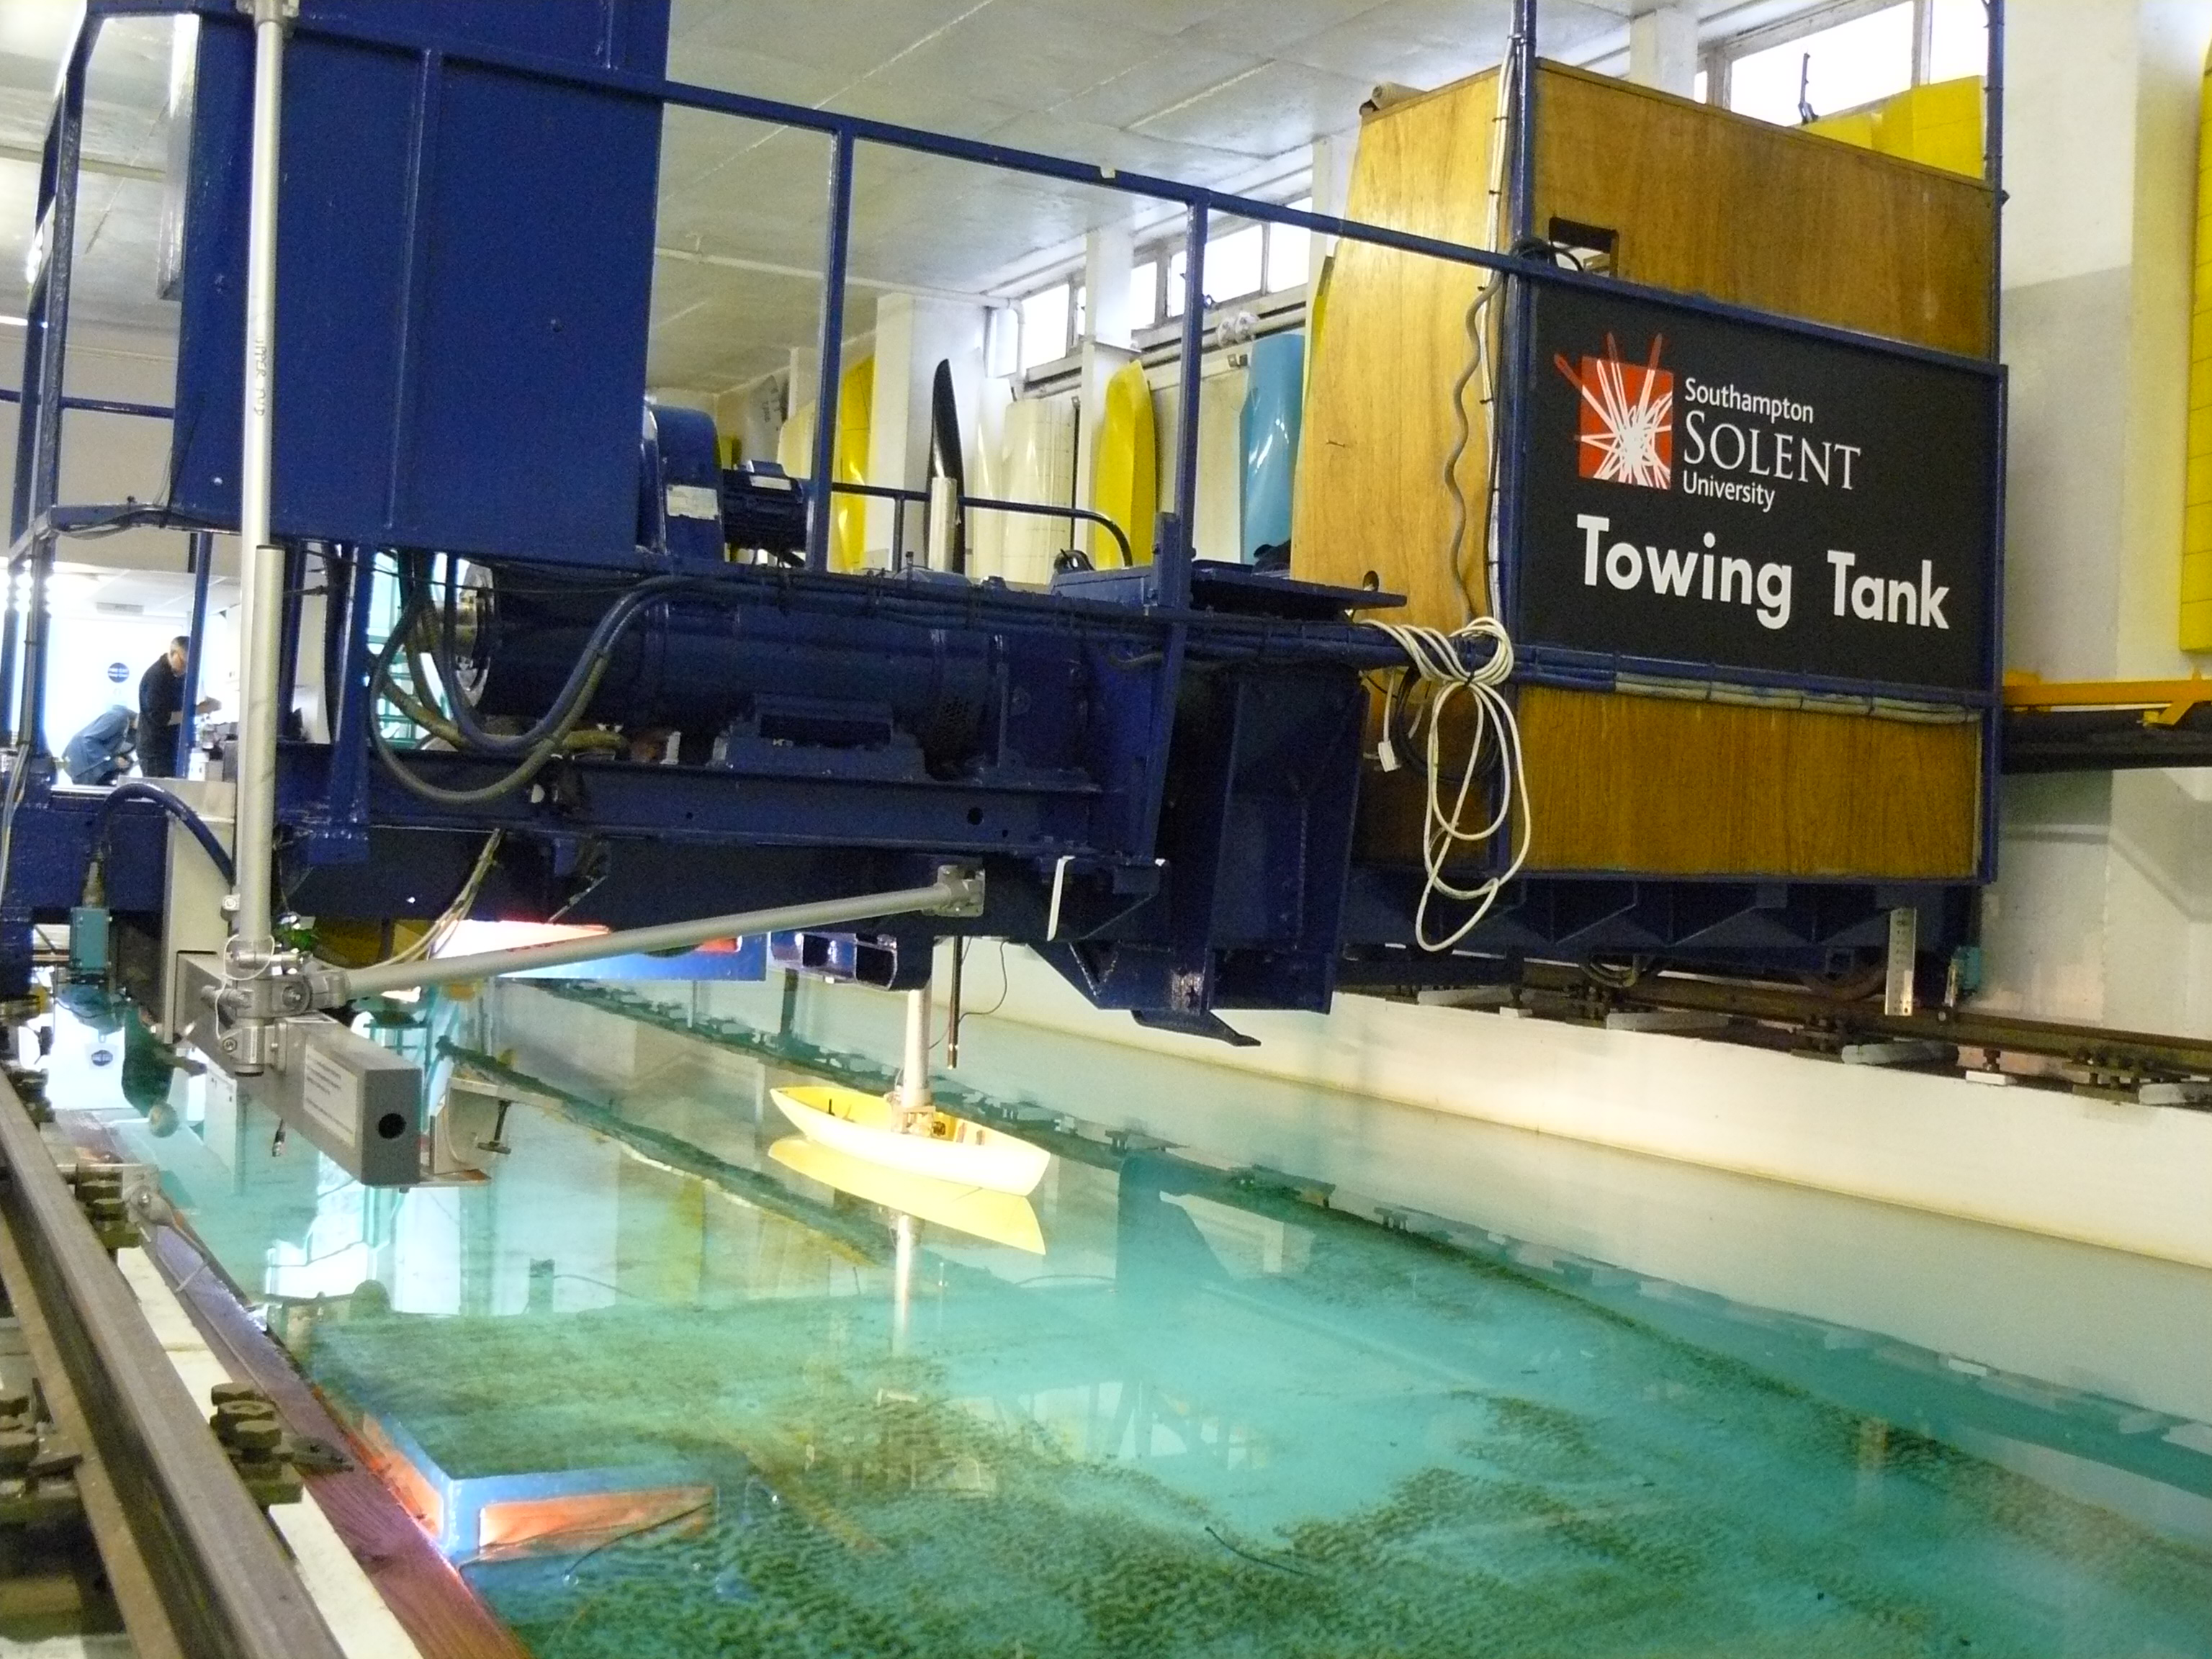
\includegraphics[height=3.5cm]{1_stat_models/figures/carene2} &
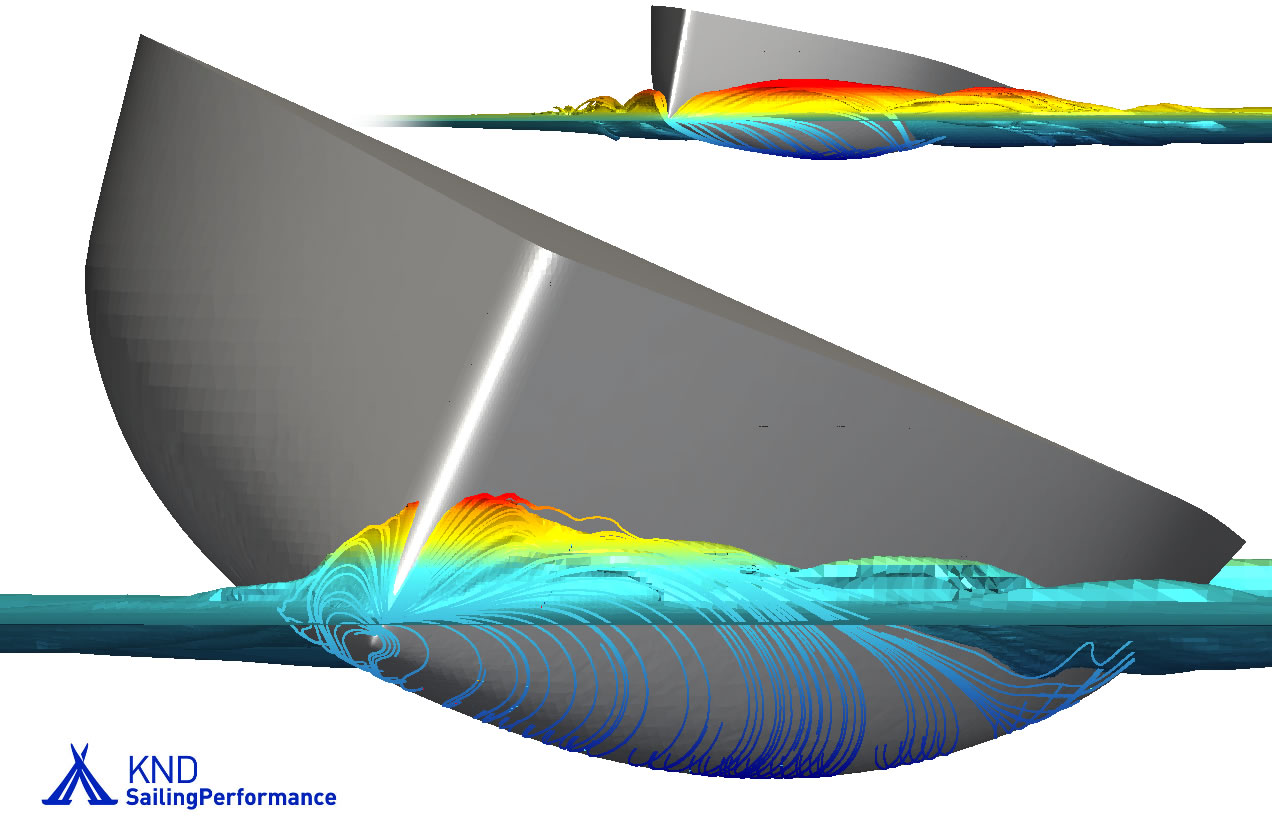
\includegraphics[height=3.5cm]{1_stat_models/figures/waterflow}
\end{tabular}
\end{center}
\end{exampleblock}
\end{frame}

%%%%%%%%%%%%%%%%%%%%%%%%%%%%%%%%%%%%%%%%%%%%%%%%%%%%%%
\begin{frame}{}
\begin{exampleblock}{Example: volcano internal structure identification}
\begin{center}
\begin{tabular}{cc}
real \vspace{1.cm} & numerical \\
\begin{minipage}[b]{0.5\textwidth}
\begin{center}
%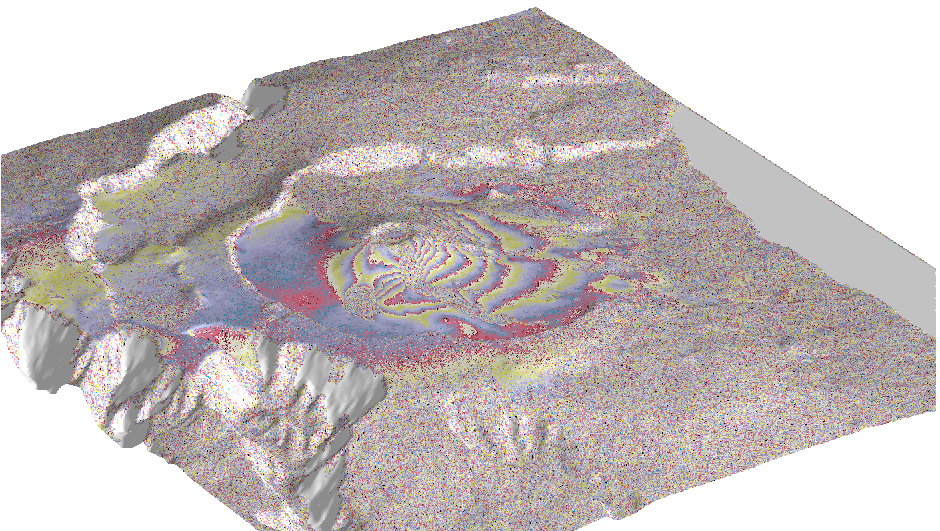
\includegraphics[width=\textwidth]{1_stat_models/figures/piton_fournaise_5dike_intrusions_98_00} \\
%{\tiny displacements resulting from 5 dike intrusions in the Piton de la Fournaise between 1998 and 2000}
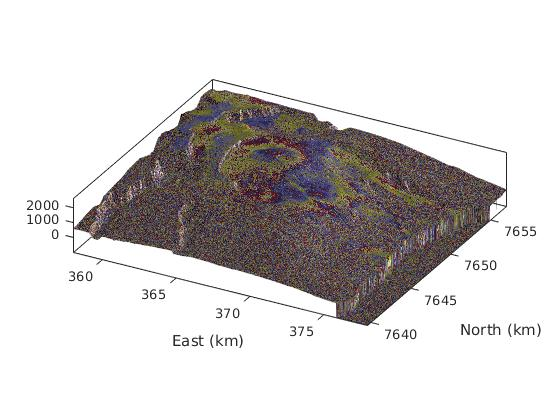
\includegraphics[width=\textwidth]{1_stat_models/figures/Interfero_Pdf_mnt_persp} \\
\vspace{0.0cm}
{\tiny Range change measured prior to the May 2016 Piton de la Fournaise eruption.
It may correspond to a source inflation + a stratisfied atmospheric signal. \\
(thanks J.-L. Froger)}
\end{center}
\end{minipage} &
\begin{minipage}[b]{0.35\textwidth}
\begin{center}
%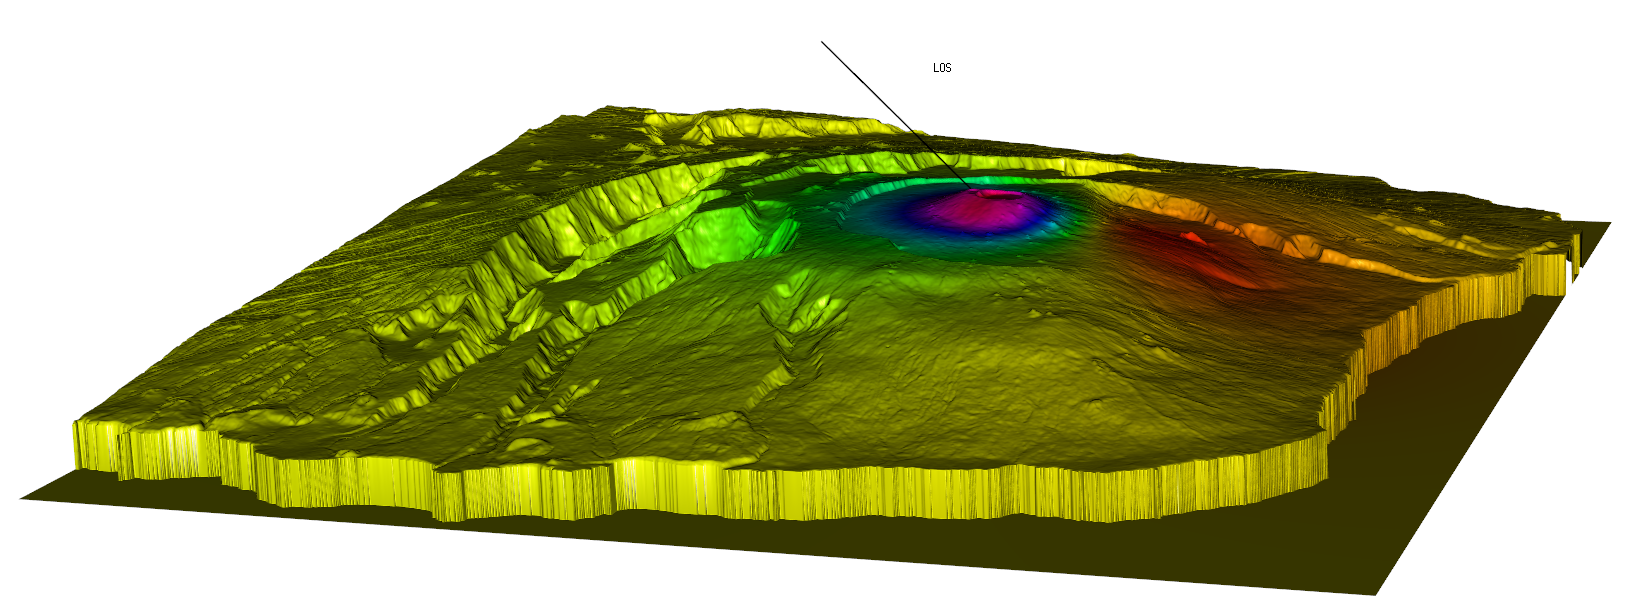
\includegraphics[height=2.7cm]{1_stat_models/figures/piton_ulos_2}
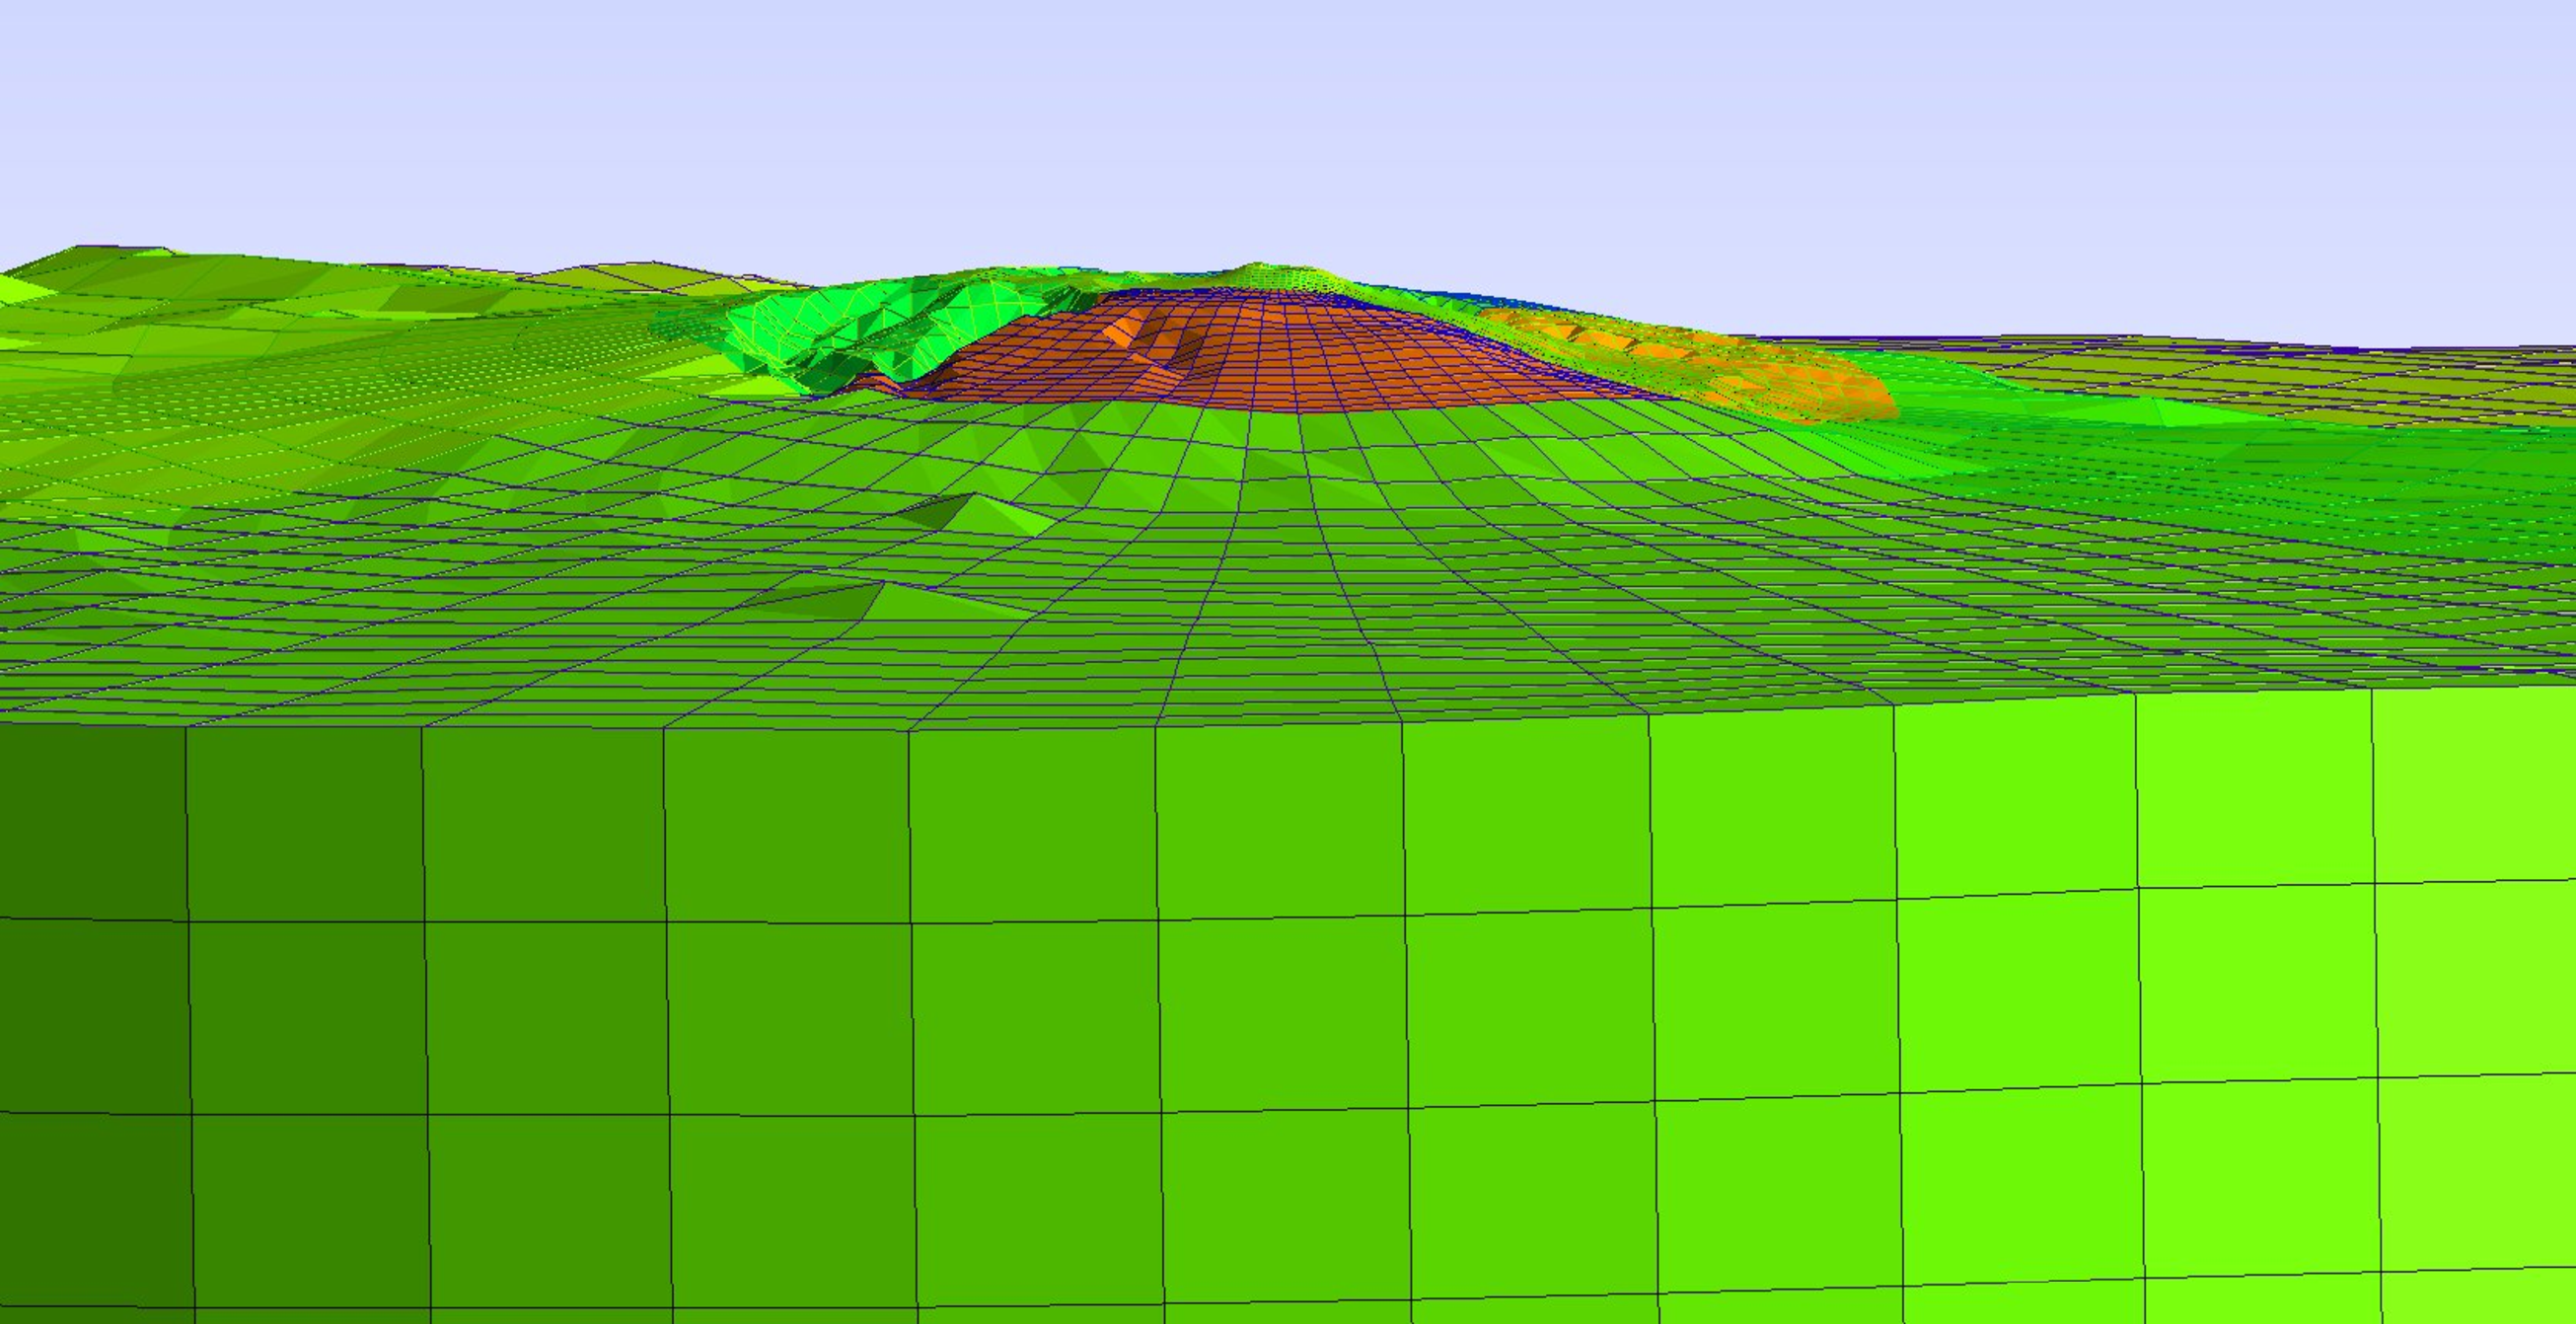
\includegraphics[width=\textwidth]{1_stat_models/figures/gmsh_mesh_piton.pdf} \\
\vspace{1.0cm}
{\tiny Finite elements mesh of the Piton de la Fournaise. \\
(thanks V. Cayol)}
\end{center}
\end{minipage} 
\\
\end{tabular}
\end{center}
\end{exampleblock}
\end{frame}

%%%%%%%%%%%%%%%%%%%%%%%%%%%%%%%%%%%%%%%%%%%%%%%%%%%%%%
%\begin{frame}{}
%\begin{exampleblock}{Example: real world experiments}
%\begin{center}
%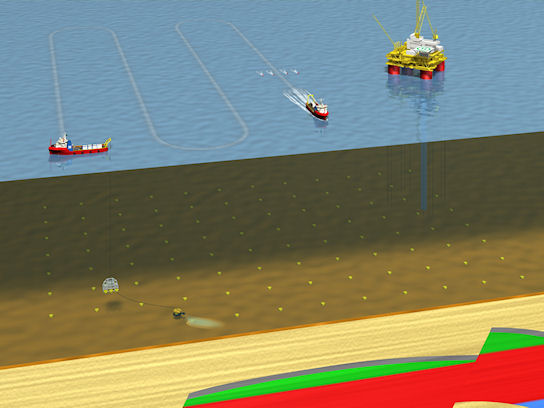
\includegraphics[height=5cm]{1_stat_models/figures/drilling}
%\end{center}
%\end{exampleblock}
%\end{frame}

%%%%%%%%%%%%%%%%%%%%%%%%%%%%%%%%%%%%%%%%%%%%%%%%%%%%%%
%\begin{frame}{}
%\begin{exampleblock}{Example: Destructive tests}
%\begin{center}
%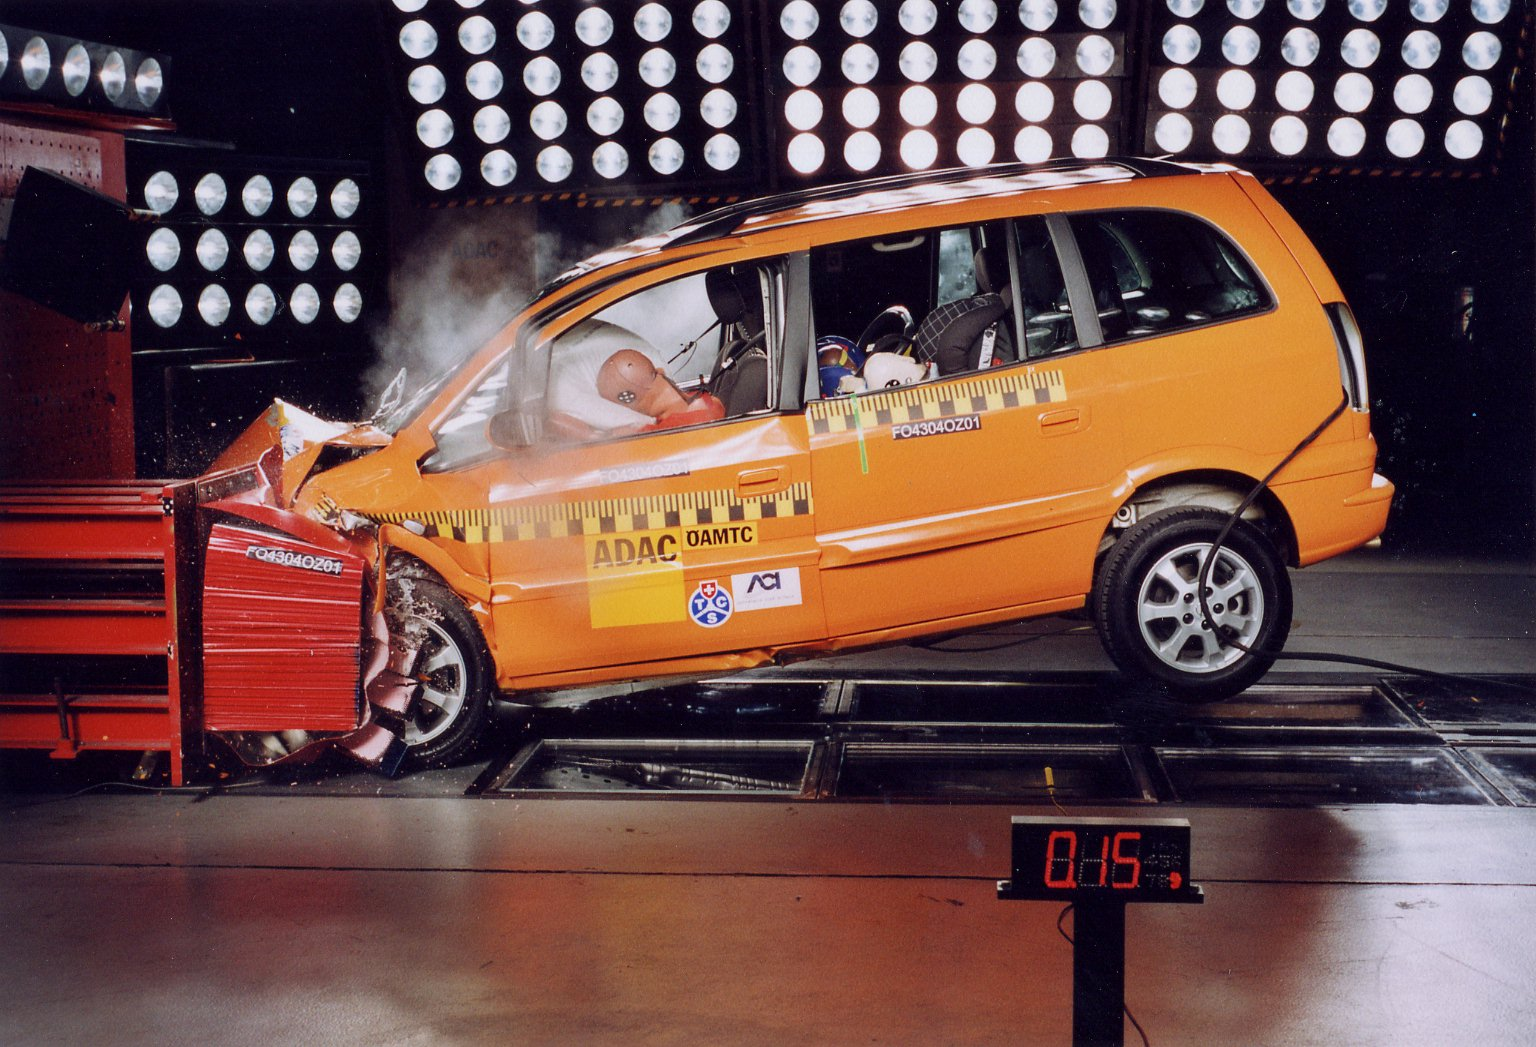
\includegraphics[height=5cm]{1_stat_models/figures/crash-test}
%\end{center}
%\end{exampleblock}
%\end{frame}

%%%%%%%%%%%%%%%%%%%%%%%%%%%%%%%%%%%%%%%%%%%%%%%%%%%%%%
%\begin{frame}{}
%\begin{exampleblock}{Example: Prototyping of a boat shape}
%\begin{center}
%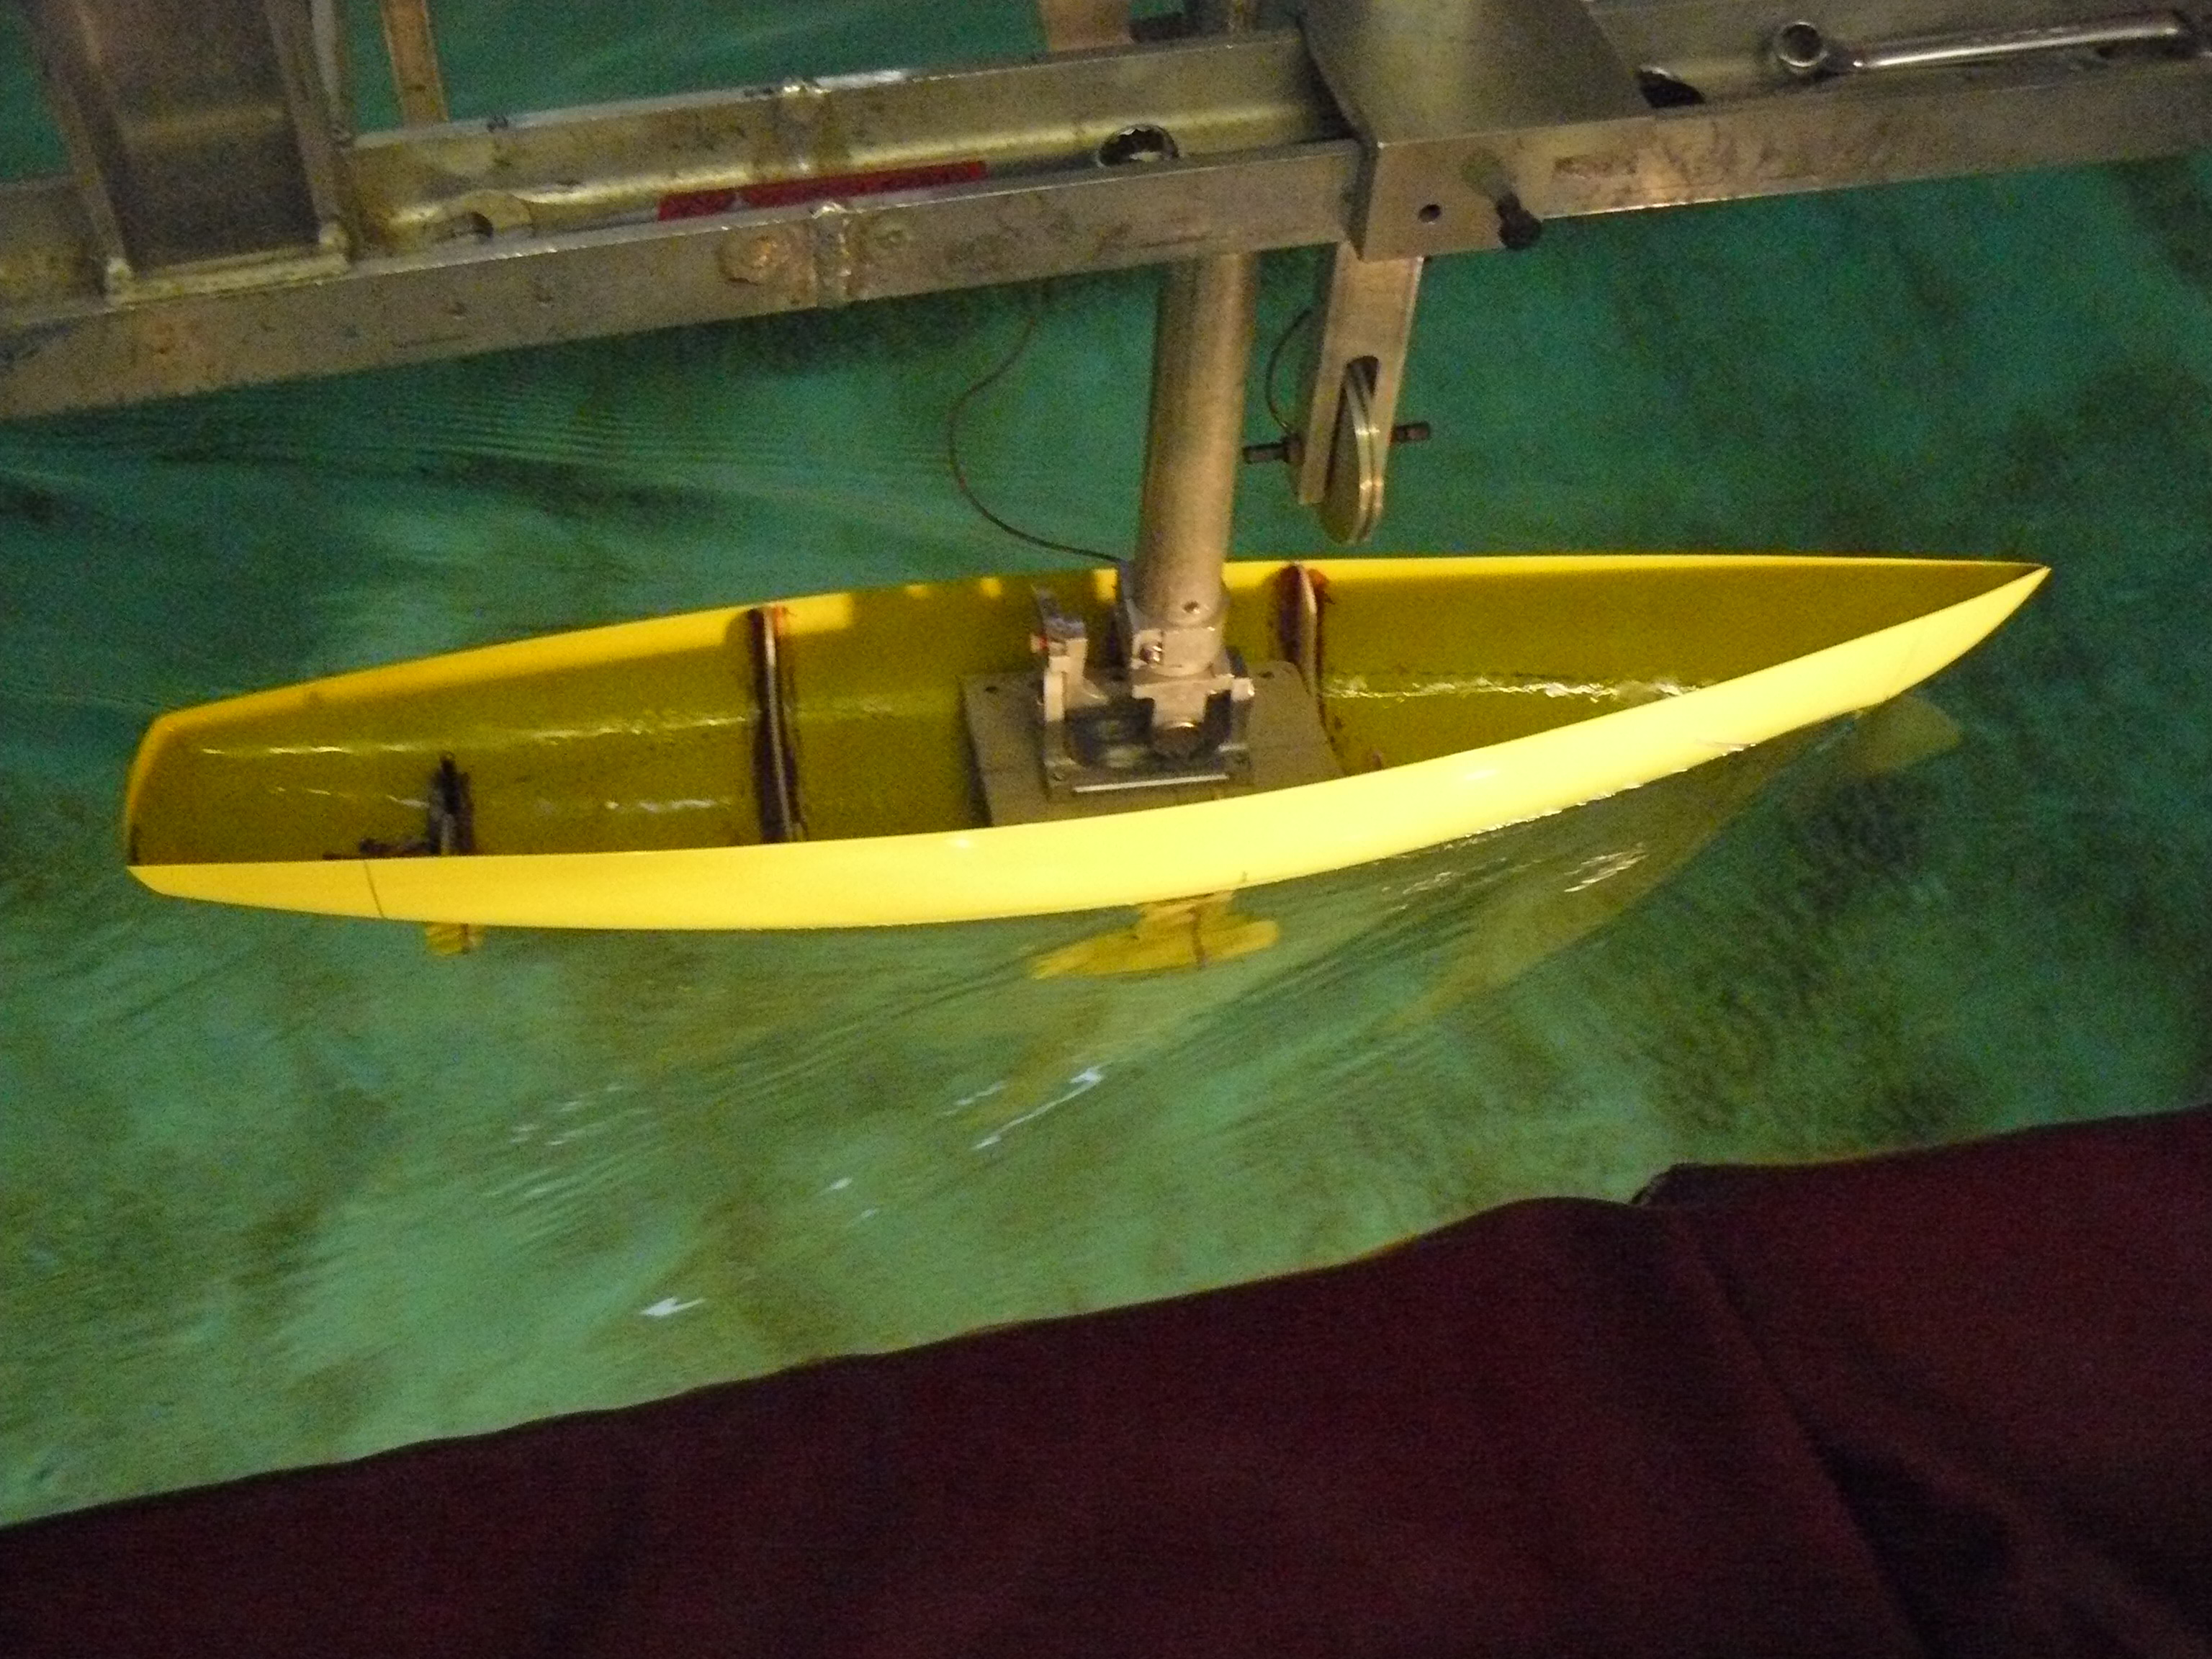
\includegraphics[height=3.5cm]{1_stat_models/figures/carene} \qquad 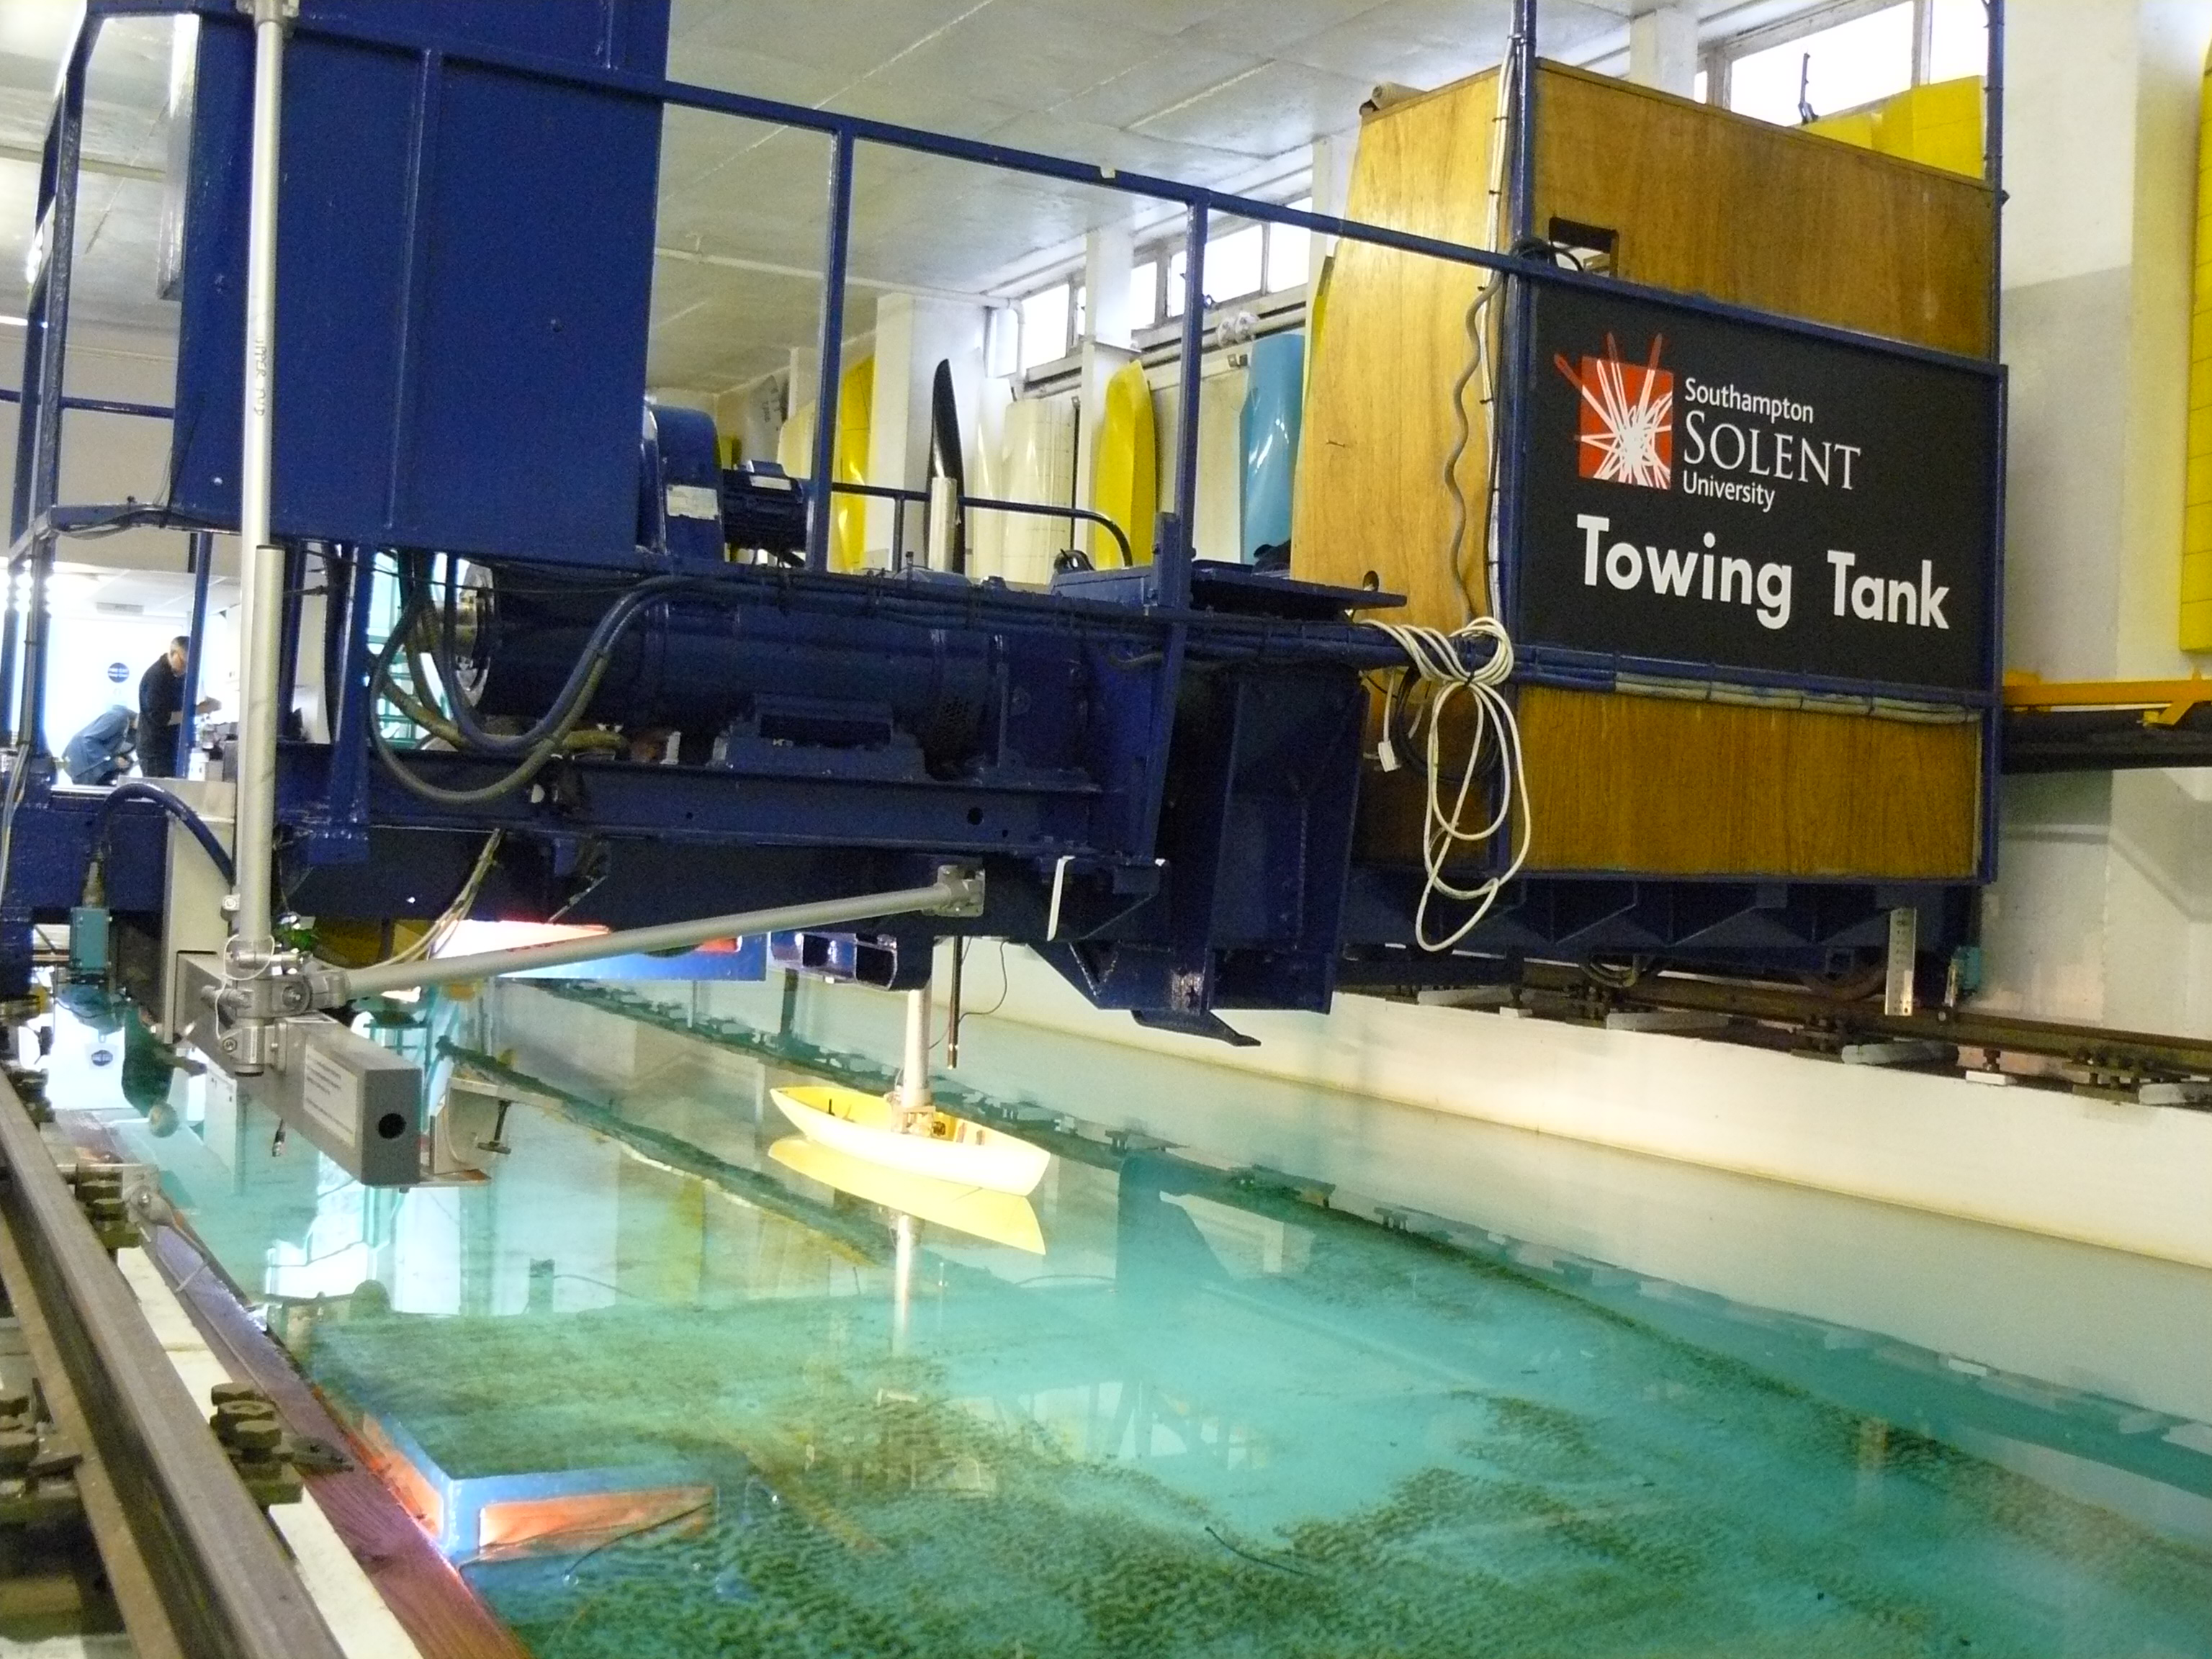
\includegraphics[height=3.5cm]{1_stat_models/figures/carene2}
%\end{center}
%Knowing the drag for a given design requires costly experiments
%\end{exampleblock}
%\end{frame}

%%%%%%%%%%%%%%%%%%%%%%%%%%%%%%%%%%%%%%%%%%%%%%%%%%%%%%
%\begin{frame}{}
%\begin{exampleblock}{Example: Numerical experiments}
%\begin{center}
%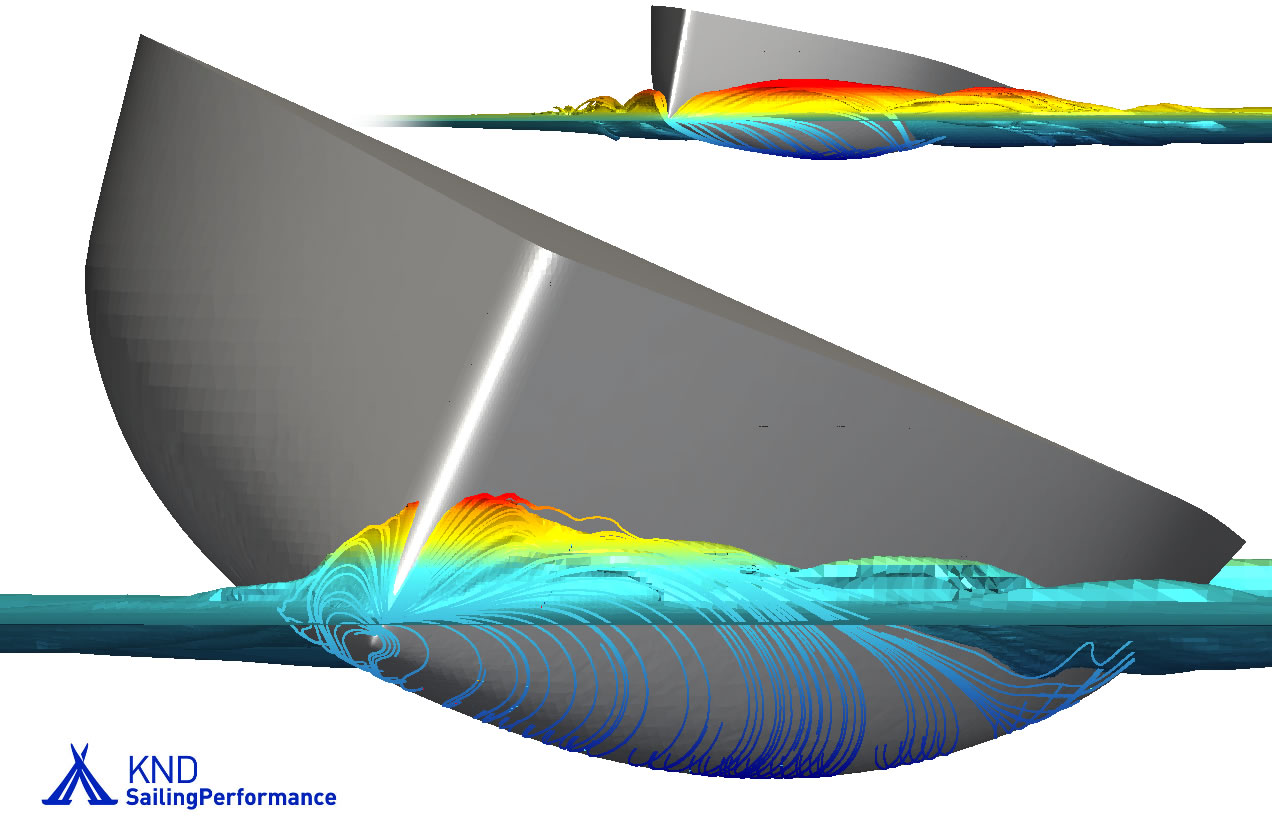
\includegraphics[height=2.8cm]{1_stat_models/figures/waterflow} \qquad 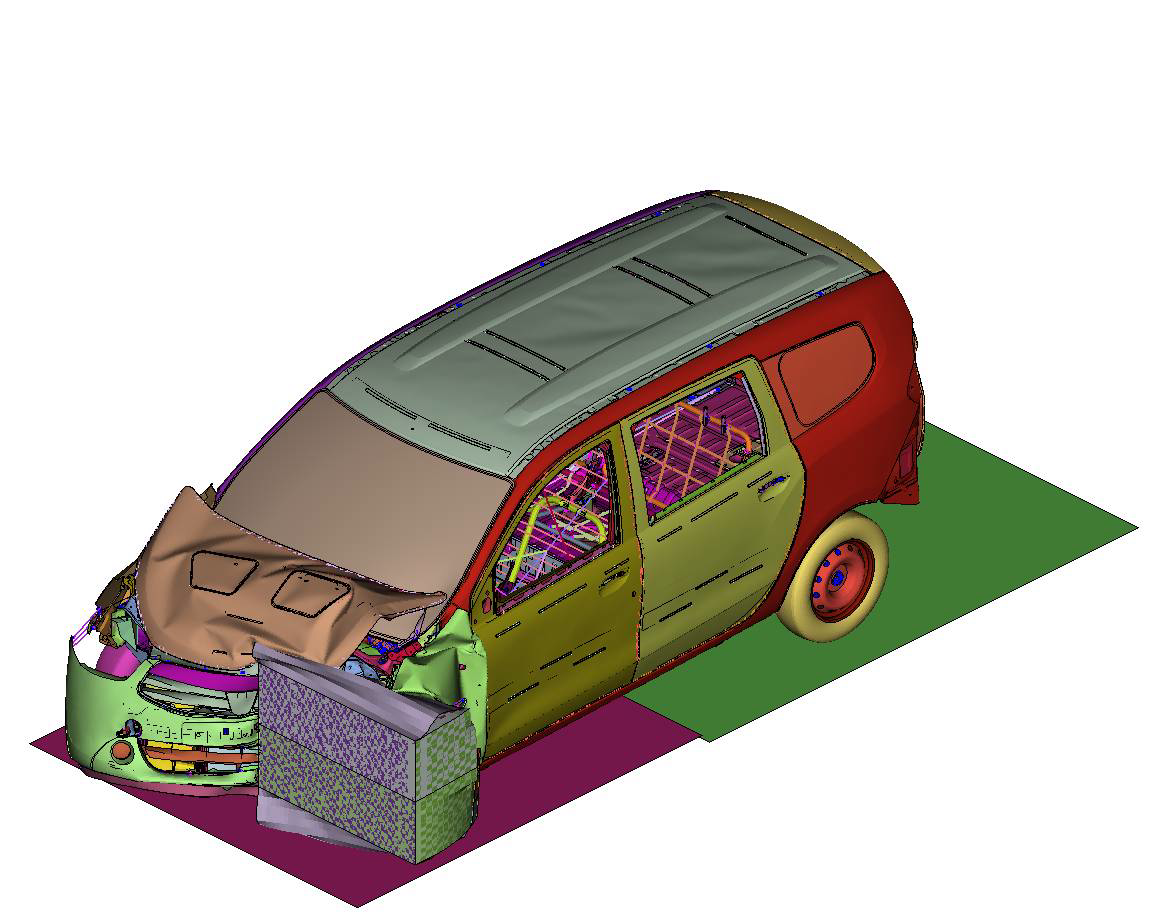
\includegraphics[height=4.2cm]{1_stat_models/figures/crash/image15}
%\end{center}
%Numerical experiments are less expensive but can be very time consuming! (expl.: 15 min / execution, 5 parameters, a grid with 10 levels, 
%total time = $10^5 \times 15$ min $>$ 2 years and 10 months)
%\end{exampleblock}
%\end{frame}

%%%%%%%%%%%%%%%%%%%%%%%%%%%%%%%%%%%%%%%%%%%%%%%%%%%%%%
\begin{frame}{}
In all these cases, the quantity of interest (drag, misfit \dots) can be seen as a function of the input parameters

$$ y = f(X) $$
where $f$ is a \textbf{costly to evaluate function}. \\
\vspace{5mm}
In the following, we will assume that
\begin{itemize}
	\item $X \in \mathds{R}^d$: There are $d$ input variables,
	\item $y \in \mathds{R}$: The output is a scalar.
\end{itemize}
\end{frame}

%%%%%%%%%%%%%%%%%%%%%%%%%%%%%%%%%%%%%%%%%%%%%%%%%%%%%%
\begin{frame}{}
The fact that $f$ is \textbf{costly to evaluate} changes a lot of things...\\
\vspace{5mm}
\structure{1. Representing the function is not possible...}\\
\vspace{5mm}
\begin{center}
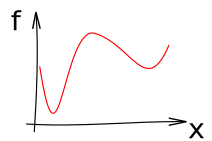
\includegraphics[height=3.2cm]{1_stat_models/figures/ink_f} 
\includegraphics[height=3.2cm]{1_stat_models/figures/Rightarrow} 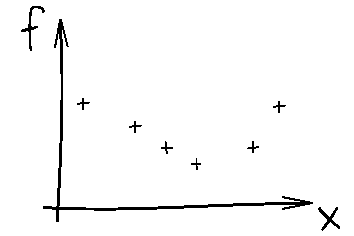
\includegraphics[height=3.2cm]{1_stat_models/figures/ink_fX}
\end{center}
\end{frame}

%%%%%%%%%%%%%%%%%%%%%%%%%%%%%%%%%%%%%%%%%%%%%%%%%%%%%%
\begin{frame}{}
The fact that $f$ is \textbf{costly to evaluate} changes a lot of things...\\
\vspace{5mm}
\structure{2. Computing integrals is not possible...}\\
\vspace{5mm}
\begin{center}
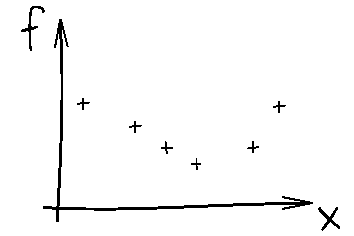
\includegraphics[height=4.5cm]{1_stat_models/figures/ink_fX}
\end{center}
What is the mean value of $f$?
\end{frame}

%%%%%%%%%%%%%%%%%%%%%%%%%%%%%%%%%%%%%%%%%%%%%%%%%%%%%%
\begin{frame}{}
The fact that $f$ is \textbf{costly to evaluate} changes a lot of things...\\
\vspace{5mm}
\structure{3. Uncertainty propagation is not possible...}\\
\vspace{5mm}
\begin{center}
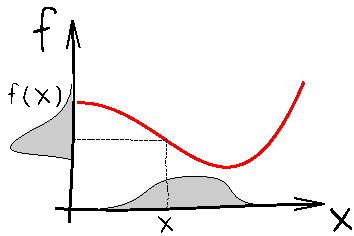
\includegraphics[height=3.2cm]{1_stat_models/figures/ink_unprogf} 
\includegraphics[height=3.2cm]{1_stat_models/figures/Rightarrow} 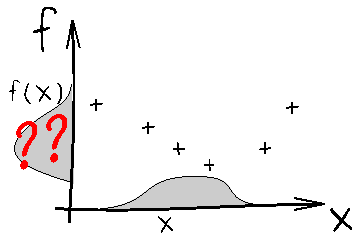
\includegraphics[height=3.2cm]{1_stat_models/figures/ink_unprogfX}
\end{center}
\end{frame}

%%%%%%%%%%%%%%%%%%%%%%%%%%%%%%%%%%%%%%%%%%%%%%%%%%%%%%
\begin{frame}{}
The fact that $f$ is \textbf{costly to evaluate} changes a lot of things...\\
\vspace{5mm}
\structure{4. Sensitivity analysis is not possible...}\\
\vspace{5mm}
\begin{center}
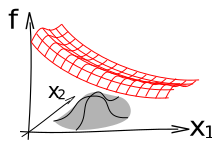
\includegraphics[height=4.5cm]{1_stat_models/figures/ink_as}
\end{center}
\end{frame}

%%%%%%%%%%%%%%%%%%%%%%%%%%%%%%%%%%%%%%%%%%%%%%%%%%%%%%
\begin{frame}{}
The fact that $f$ is \textbf{costly to evaluate} changes a lot of things...\\
\vspace{5mm}
\structure{5. Optimisation is also tricky...}\\
\vspace{5mm}
\begin{center}
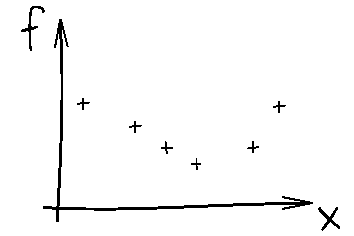
\includegraphics[height=4.5cm]{1_stat_models/figures/ink_fX}
\end{center}
\end{frame}

%%%%%%%%%%%%%%%%%%%%%%%%%%%%%%%%%%%%%%%%%%%%%%%%%%%%%%
\begin{frame}{}
The principle of statistical modelling is to use the data to build a mathematical approximation of the function.
\begin{center}
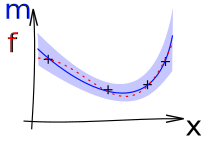
\includegraphics[height=4.5cm]{1_stat_models/figures/ink_m}
\end{center}
The model can then be used to answer all previous questions
\end{frame}

%%%%%%%%%%%%%%%%%%%%%%%%%%%%%%%%%%%%%%%%%%%%%%%%%%%%%%
\begin{frame}{}
Of course, there is a difference between $f$ and $m$...
\begin{center}
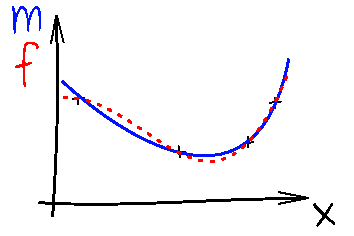
\includegraphics[height=5cm]{1_stat_models/figures/ink_mf}
\end{center}
\end{frame}

%%%%%%%%%%%%%%%%%%%%%%%%%%%%%%%%%%%%%%%%%%%%%%%%%%%%%%
\begin{frame}{}
Why \textbf{statistical models}? \\We want to be able to quantify the model error:
\begin{center}
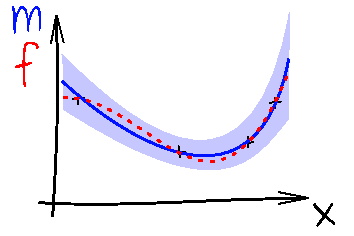
\includegraphics[height=5cm]{1_stat_models/figures/ink_mconfint}
\end{center}
The confidence intervals can be used to obtain a \textbf{measure of uncertainty on the value of interest}.
\end{frame}

%%%%%%%%%%%%%%%%%%%%%%%%%%%%%%%%%%%%%%%%%%%%%%%%%%%%%%
\begin{frame}{}
In the sequel, we will use the following notations :
\begin{itemize}
	\item The set of observation points will be represented by a $n \times d$ matrix $X=(X_1, ..., X_n)^t$
	\item The vector of observations will be denoted by $F$ : $F_i=f(X_i)$ (or $F=f(X)$).
\end{itemize}
There are many surrogate methods available on the market
\begin{itemize}
	\item Linear regression
	\item Smoothing splines
	\item Gaussian process regression
	\item Neural Networks
    \item ...
\end{itemize}
In this course we will focus on \textbf{Gaussian Process Regression}. \\
{\tiny (This notation may a few times be ambiguous as $X$ will also denote the random variable associated to $x$
but the context should allow understanding)}
\end{frame}

%%%%%%%%%%%%%%%%%%%%%%%%%%%%%%%%%%%%%%%%%%%%%%%%%%%%%%
\begin{frame}{}
Two breadcrumb examples related to the \textbf{identification of a spherical magma reservoir from measured displacements } along a satellite line of sight:
\vskip\baselineskip
\begin{minipage}[b]{0.45\textwidth}
{\color{blue}1)} the processing of surface measures for \textit{i)} reconstructing missing measures and \textit{ii)} denoising,
\end{minipage} 
\hspace{0.4cm}
\begin{minipage}[b]{0.45\textwidth}
{\color{blue}2)} minimizing the missfit between a Mogi model of a spherical reservoir and the surface measures.
\end{minipage}
\begin{center}
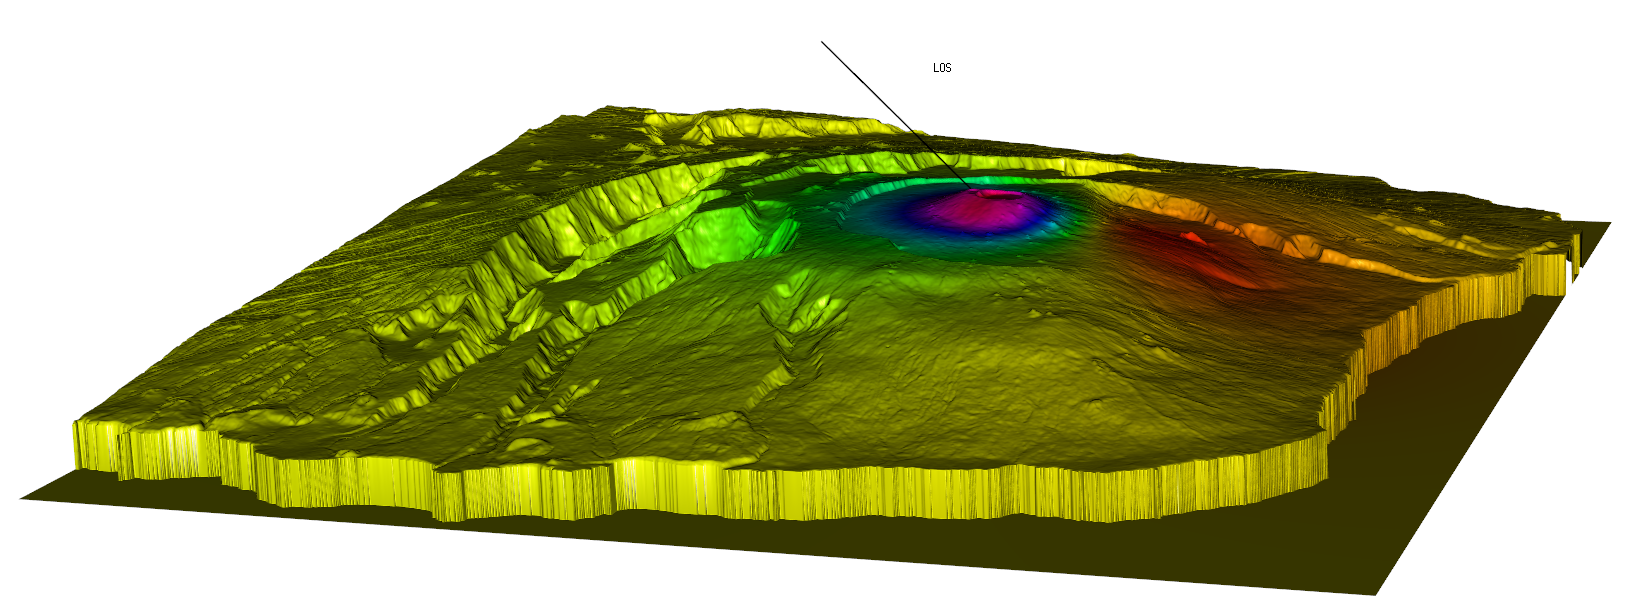
\includegraphics[width=0.7\textwidth]{1_stat_models/figures/piton_ulos_2}
\end{center}
\end{frame}

%%%%%%%%%%%%%%%%%%%%%%%%%%%%%%%%%%%%%%%%%%%%%%%%%%%%%%
\begin{frame}{}
\textbf{Misfit minimization problem}:
\begin{equation*}
\begin{split}
& \min_{x \in [x^L,x^U] \subset \mathds{R}^d} f(x) \quad \text{ where the misfit is}\\
& ~ f(x) ~=~\frac{1}{2} (U(x) - U^{m})^\top C^{-1} (U(x) - U^{m})
\end{split}
\end{equation*}
\begin{itemize}
\item $U^m$: $m \times 1$ displacements projected on the line of sight.
\item $U(x)$: $m \times 1$ Mogi model displacements projected on the line of sight.
\item $x$: identification variables, the coordinates, radius and overpressure of a spherical magma reservoir, $x = \{xs,ys,zs,a,p\}$, resp.
\item $C$: $m \times m$ covariance matrix of the measures.
\end{itemize}
\end{frame}

%%%%%%%%%%%%%%%%%%%%%%%%%%%%%%%%%%%%%%%%%%%%%%%%%%%%%%
\begin{frame}{}
\textbf{Misfit minimization problem}: \\
$\Rightarrow$ demo with \texttt{plots\_3d\_full\_grid.R}
\begin{center}
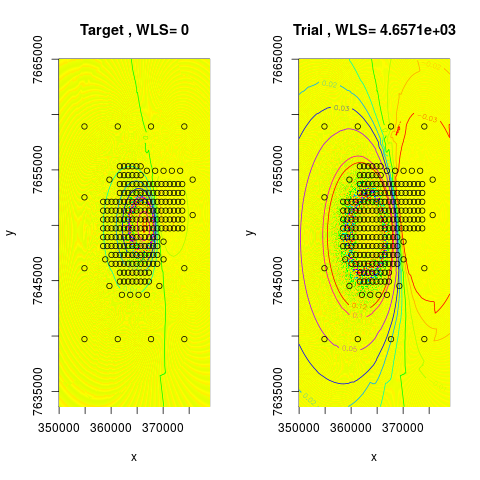
\includegraphics[width=0.6\textwidth,height=0.6\textheight]{1_stat_models/figures/contour_ulos_compare}
\end{center}
{\tiny The bullets are the $m=220$ measure locations (under-sampled from the full grid with the quadtree method). \\ 
target reservoir (left): $xs= 367000$, $ys= 7650300$, $zs=0$ (UTM $m$), $a=500~m$, $p=20~MPa$.\\
trial reservoir (right): $xs= 365000$, $ys= 7649800$, $zs=-2000$ (UTM $m$), $a=500~m$, $p=300~MPa$.\\
}
\end{frame}

%%%%%%%%%%%%%%%%%%%%%%%%%%%%%%%%%%%%%%%%%%%%%%%%%%%%%%
%%%%%%%%%%%%%%%%%%%%%%%%%%%%%%%%%%%%%%%%%%%%%%%%%%%%%%
\section[Gaussian Process regression]{Gaussian Process Regression}
\subsection{}
%%%%%%%%%%%%%%%%%%%%%%%%%%%%%%%%%%%%%%%%%%%%%%%%%%%%%%
\begin{frame}{}
\vspace{0.75cm}
\structure{This section is organised in 3 subsections:}
\vspace{0.5cm}
\begin{enumerate}
    \item Univariate and multivariate normal distributions
    \item Gaussian processes
    \item Gaussian process regression
\end{enumerate}
\end{frame}

%%%%%%%%%%%%%%%%%%%%%%%%%%%%%%%%%%%%%%%%%%%%%%%%%%%%%%%%%%%%
%\subsection{Multivariate normal distribution}

%%%%%%%%%%%%%%%%%%%%%%%%%%%%%%%%%%%%%%%%%%%%%%%%%%%%%%
\begin{frame}{1D normal distribution}
We say that $X \sim \mathcal{N}(\mu,\sigma^2)$ if it has the following pdf:
\begin{columns}
  \begin{column}{0.6\textwidth}
  \begin{equation*}
  f(x) = \frac{1}{\sigma \sqrt{2 \pi}} \exp \left(-\frac{(x-\mu)^2}{2 \sigma^2} \right)
  \vspace{3mm}
  \end{equation*}
  The distribution is characterised by\\
      \qquad mean: $\mu = \E [X]$\\
      \qquad variance: $\sigma^2 = \E [X^2] - \E[X]^2$
  \end{column}
  \begin{column}{0.5\textwidth}
  \begin{center}
   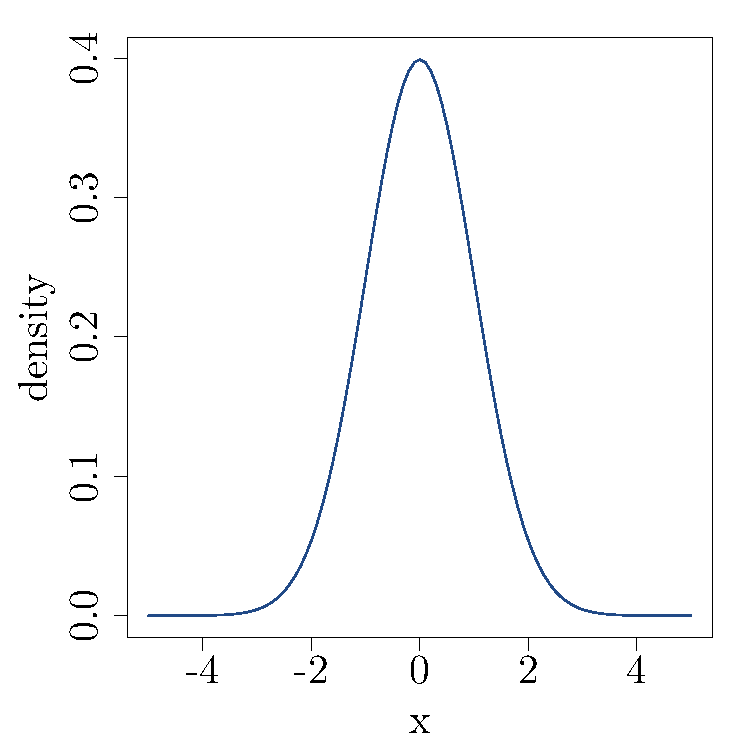
\includegraphics[height=4.7cm]{1_stat_models/figures/R/MVN_dens1} 
  \end{center}
  \end{column}
\end{columns}
\vspace{2mm}
\structure{One fundamental property:} a linear combination of independant normal distributed random variables is still normal distributed.
\end{frame}

%%%%%%%%%%%%%%%%%%%%%%%%%%%%%%%%%%%%%%%%%%%%%%%%%%%%%%
\begin{frame}{Multivariate normal distribution}
\begin{definition}
	We say that a vector $Y=(Y_1, \dots, Y_d)^t$ follows a multivariate normal distribution if any linear combination of $Y$ follows a normal distribution:
	\begin{equation*}
		\forall \alpha \in \mathds{R}^d,\ \alpha^t Y \sim \mathcal{N}
	\end{equation*}
\end{definition}
The distribution of a Gaussian vector is characterised by
\begin{itemize}
 	\item a \textbf{mean vector} $\mu = \E [Y]$
 	\item a \textbf{covariance matrix} $\Sigma = \E[YY^t] - \E[Y] \E[Y]^t$ % \hfill (i.e. $\Sigma_{i,j}=\Cov(Y_i, Y_j)$)
\end{itemize}
\vspace{3mm}
\structure{Property:}\\
A covariance matrix is
\begin{itemize}
	\item symmetric $K_{i,j}=K_{j,i}$
	\item positive semi-definite $\forall \alpha \in \mathds{R}^d, \alpha^t K \alpha \geq 0$.
\end{itemize}
\end{frame}

%%%%%%%%%%%%%%%%%%%%%%%%%%%%%%%%%%%%%%%%%%%%%%%%%%%%%%
\begin{frame}{}
The density of a multivariate Gaussian is:
\begin{equation*}
f_Y(x) = \frac{1}{\displaystyle (2 \pi)^{d/2} |\Sigma|^{1/2}} \exp \left(-\frac12 (x-\mu)^t \Sigma^{-1} (x-\mu)  \right).
\end{equation*}
\begin{center}
 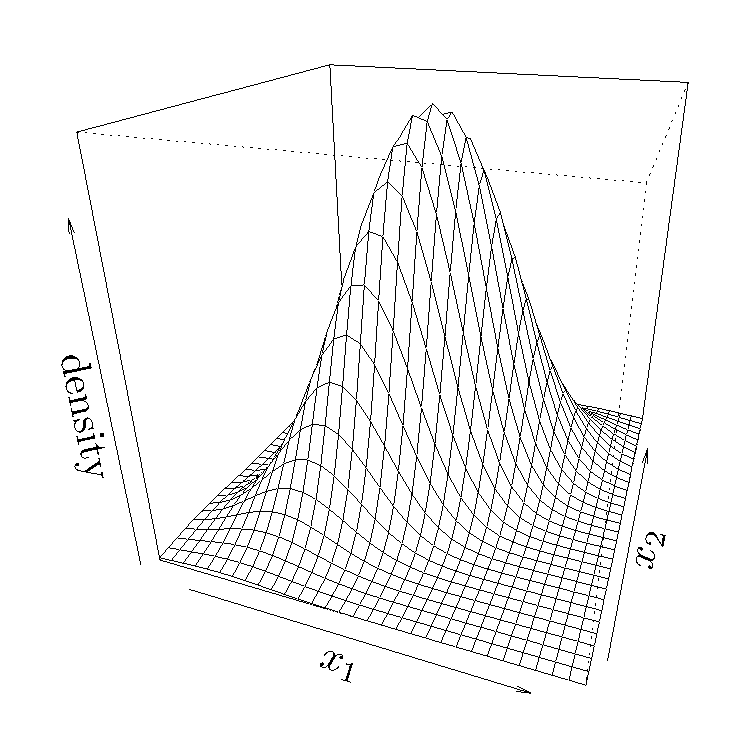
\includegraphics[height=5cm]{1_stat_models/figures/R/MVN_dens2}
\end{center}
\end{frame}


%%%%%%%%%%%%%%%%%%%%%%%%%%%%%%%%%%%%%%%%%%%%%%%%%%%%%%
\begin{frame}{}
\begin{exampleblock}{Samples from a multivariate normal}
 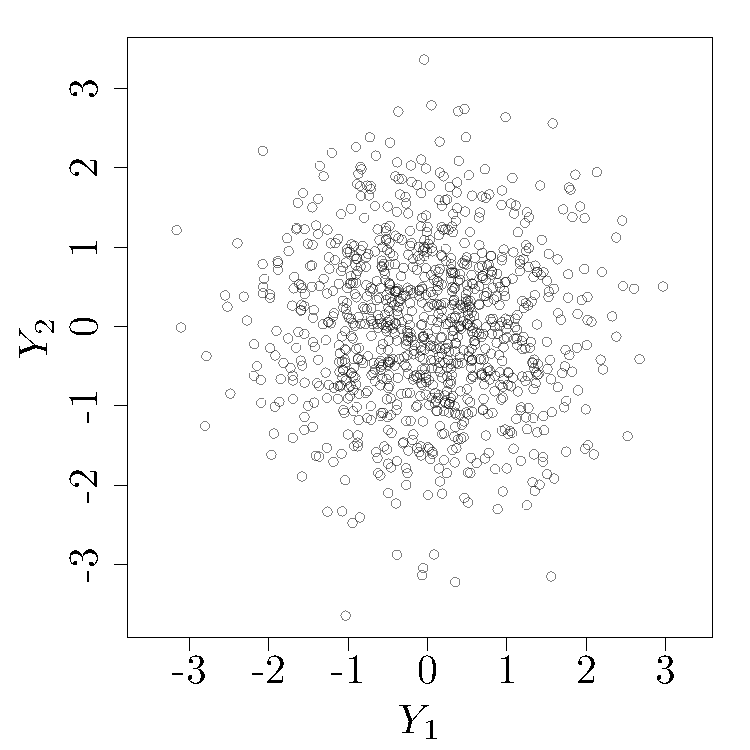
\includegraphics[height=4.5cm]{1_stat_models/figures/R/MVN_gaussvec2} \qquad \qquad 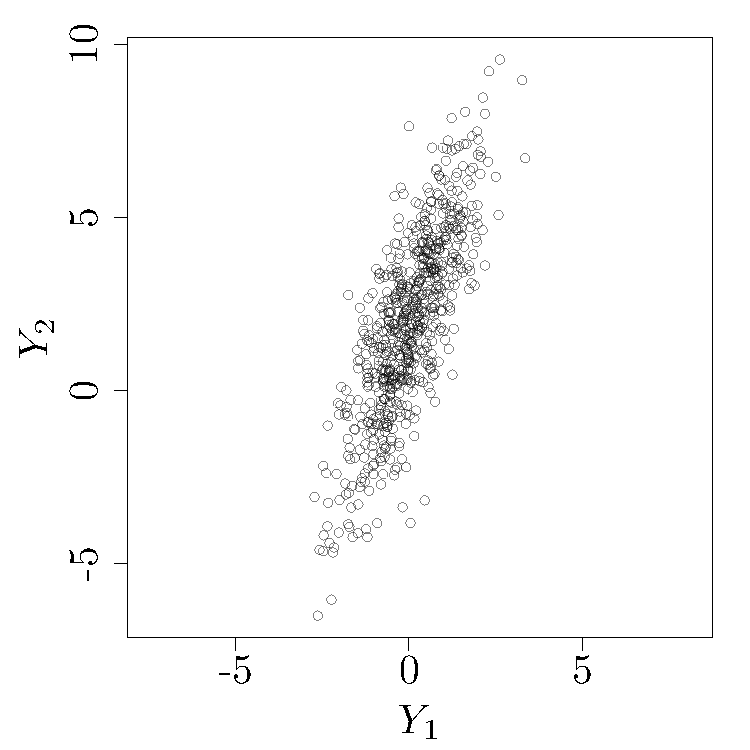
\includegraphics[height=4.5cm]{1_stat_models/figures/R/MVN_gaussvec1}
\end{exampleblock}
\vspace{-5mm}
\begin{exampleblock}{Exercise}
\begin{itemize}
  \item For $X=(X_1,\dots,X_d)$ with $X_i$ independant and $\mathcal{N}(0,1)$, and a $d \times d$ matrix $A$, what is the distribution of $AX$?
  \item For a given covariance matrix $K$ and independant $\mathcal{N}(0,1)$ samples, how can we generate $\mathcal{N}(\mu,K)$ random samples?
\end{itemize}
\end{exampleblock}
\alert{$\Rightarrow$ R demo}
\end{frame}

%%%%%%%%%%%%%%%%%%%%%%%%%%%%%%%%%%%%%%%%%%%%%%%%%%%%%%
\begin{frame}{}
\begin{exampleblock}{Counter example}
\begin{center}
 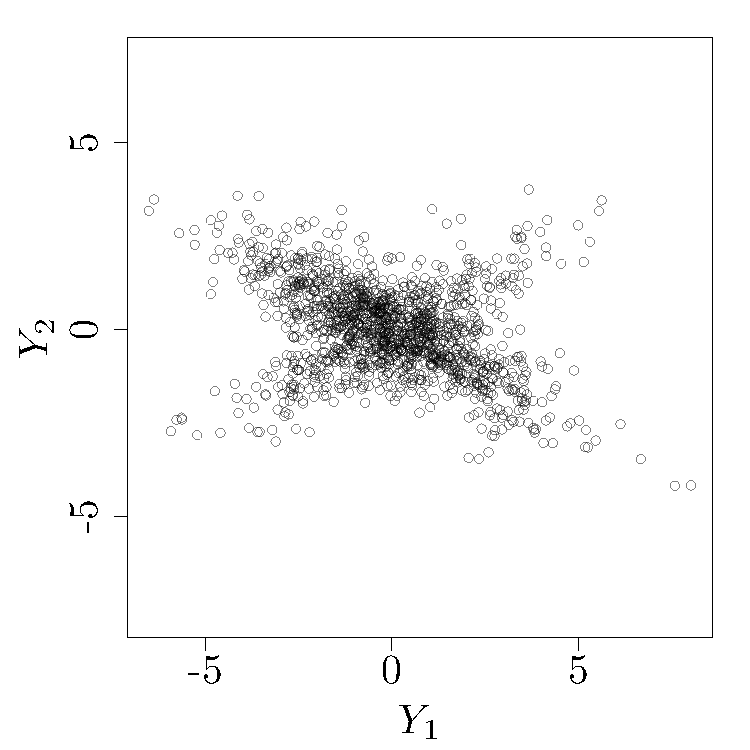
\includegraphics[height=5cm]{1_stat_models/figures/R/MVN_gaussvec3}
\end{center}
$Y_1$ and $Y_2$ are normally distributed but \textbf{the couple $(Y_1,Y_2)$ is not}.
\end{exampleblock}
\end{frame}


%%%%%%%%%%%%%%%%%%%%%%%%%%%%%%%%%%%%%%%%%%%%%%%%%%%%%%
\begin{frame}{}
\begin{block}{Conditional distribution}
2D multivariate Gaussian conditional distribution:\\
\begin{center}
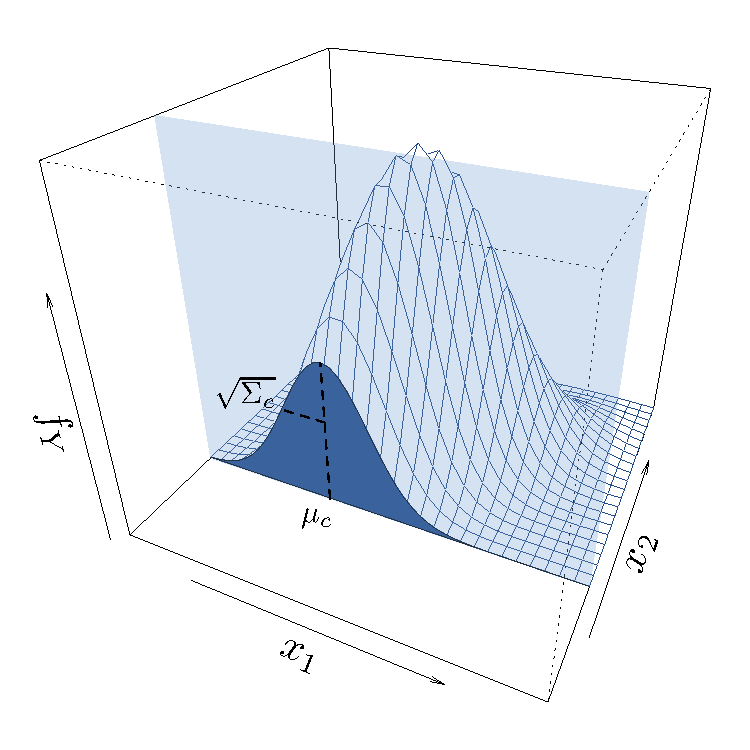
\includegraphics[height=6cm]{1_stat_models/figures/ch1_condpdf1}
\end{center}
The conditional distribution is still Gaussian!
\end{block}
\end{frame}

%%%%%%%%%%%%%%%%%%%%%%%%%%%%%%%%%%%%%%%%%%%%%%%%%%%%%%
\begin{frame}{}
\begin{block}{Conditional distribution}
Let $(Y,Z)$ be a Gaussian vector ($Y$ and $Z$ may both be vectors) with mean $(\mu_Y,\mu_Z)^t$ and covariance matrix
\begin{equation*}
\begin{pmatrix}
	\Cov(Y,Y) & \Cov(Y,Z)\\
	\Cov(Z,Y) & \Cov(Z,Z)\\
\end{pmatrix}.
\end{equation*}
The conditional distribution of $Y$ knowing $Z$ is still multivariate normal $Y|Z \sim \mathcal{N}(\mu_{cond},\Sigma_{cond})$ with
\begin{equation*}
\begin{split}
	\mu_{cond} &= \E [Y|Z] = \mu_Y + \Cov(Y,Z) \Cov(Z,Z)^{-1} (Z-\mu_Z)\\
	\Sigma_{cond} &= \Cov [Y,Y|Z] = \Cov(Y,Y) - \Cov(Y,Z) \Cov(Z,Z)^{-1} \Cov(Z,Y)
\end{split}
\end{equation*}
\end{block}
\end{frame}

%%%%%%%%%%%%%%%%%%%%%%%%%%%%%%%%%%%%%%%%%%%%%%%%%%%%%%
\begin{frame}{}
\begin{exampleblock}{3D Example}
3D multivariate Gaussian conditional distribution:\\
\begin{center}
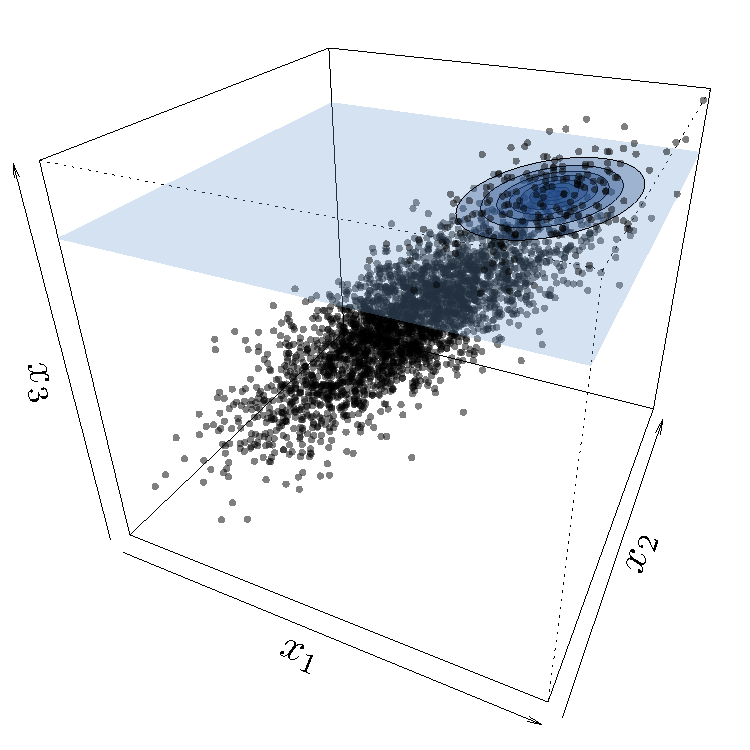
\includegraphics[height=6cm]{1_stat_models/figures/ch1_condpdf2}
\end{center}
\end{exampleblock}
\end{frame}



%%%%%%%%%%%%%%%%%%%%%%%%%%%%%%%%%%%%%%%%%%%%%%%%%%%%%%
\begin{frame}{2. Gaussian processes}
The multivariate Gaussian distribution can be generalised to random processes:
\begin{definition}
A random process $Z$ over $D \subset \mathds{R}^d$ is said to be Gaussian if
\begin{equation*}
\forall n \in \mathds{N}, \forall x_i \in D, (Z(x_1),\dots,Z(x_n)) \text{  is a Gaussian vector}.
\end{equation*}
\end{definition}
The distribution of a GP is fully characterised by:
\begin{itemize}
	\item its mean function $m$ defined over $D$
	\item its covariance function (or kernel) $k$ defined over $D \times D$: $k(x,y) = \Cov(Z(x),Z(y))$
\end{itemize}
We will use the notation $Z \sim \mathcal{N}(m(.),k(.,.))$.\\
\end{frame}

%%%%%%%%%%%%%%%%%%%%%%%%%%%%%%%%%%%%%%%%%%%%%%%%%%%%%%
\begin{frame}{}
Let's look at the sample paths of a Gaussian Process!\\
\vspace{2mm}
\alert{$\Rightarrow$ Shiny App:} \url{https://github.com/NicolasDurrande/shinyApps} \\
\vspace{5mm}
In order to simulate sample paths from a GP $Z \sim \mathcal{N}(m(.),k(.,.))$, we consider the samples discretised on a fine grid.
\vspace{5mm}
\begin{exampleblock}{Exercise: Simulating sample paths}
Let X be a set 100 regularly spaced points over the input space of $Z$.
\begin{itemize}
	\item What is the distribution of $Z(X)$ ?
	\item How to simulate samples from $Z(X)$ ?
\end{itemize}
\end{exampleblock}
\end{frame}

%%%%%%%%%%%%%%%%%%%%%%%%%%%%%%%%%%%%%%%%%%%%%%%%%%%%%%
\begin{frame}{}
A kernel satisfies the following properties:
\begin{itemize}
	\item It is symmetric: $k(x,y) = k(y,x)$
	\item It is positive semi-definite (psd):
\end{itemize}
\begin{equation*}
	\forall n \in \mathds{N}, \forall x_i \in D, \forall \alpha \in \mathds{R}^n,\  \sum_{i=1}^n \sum_{j=1}^n \alpha_i \alpha_j k(x_i,x_j) \geq 0
\end{equation*}
\vspace{5mm} \\
Furthermore any symmetric psd function can be seen as the covariance of a Gaussian process. This equivalence is known as the Loeve theorem.
\end{frame}

%%%%%%%%%%%%%%%%%%%%%%%%%%%%%%%%%%%%%%%%%%%%%%%%%%%%%%
\begin{frame}{}
There are a lot of functions that have already been proven psd:\\
\vspace{2mm}
\footnotesize
\begin{tabular}{rlN}
		constant & $ \displaystyle k(x,y) = \sigma^2 $ &\\[4mm]
		white noise & $ \displaystyle k(x,y) = \sigma^2 \delta_{x,y} $ &\\[4mm]
		Brownian & $ \displaystyle k(x,y) =  \sigma^2  \min (x,y) $ &\\[4mm]
		exponential & $\displaystyle k(x,y) =  \sigma^2 \exp \left(- |x-y|/\theta \right)$ &\\[4mm]
		Matern 3/2 & $\displaystyle k(x,y) =  \sigma^2 \left(1 + |x-y| \right) \exp \left(- |x-y| /\theta\right)$ &\\[4mm]
		Matern 5/2 & $\displaystyle k(x,y) =  \sigma^2 \left(1 + |x-y| /\theta+ 1/3|x-y|^2 /\theta^2 \right) \exp \left(- |x-y| /\theta\right)$ &\\[4mm]
		\hspace{-5mm}squared exponential & $\displaystyle k(x,y) =  \sigma^2 \exp \left(- (x-y)^2 /\theta^2 \right)$ &\\[4mm]
		$\vdots$ &
		% linear & $ \displaystyle k(x,y) = \sigma^2 xy $ &\\[4mm]
		% cosine & $ \displaystyle k(x,y) = \sigma^2 \cos \left (\frac{x-y}{\theta} \right) $ &\\[4mm]
		% sinc & $ \displaystyle k(x,y) = \sigma^2 \frac{\theta}{x-y} \sin \left( \frac{x-y}{\theta} \right) $ &\\[4mm] \hline
\end{tabular}\\
%%\begin{tabular}{rlN}
%%		constant & $ \displaystyle k(x,y) = 1 $ &\\[4mm]
%%		white noise & $ \displaystyle k(x,y) = \delta_{x,y} $ &\\[4mm]
%%		Brownian & $ \displaystyle k(x,y) =  \min (x,y) $ &\\[4mm]
%%		exponential & $\displaystyle k(x,y) = \exp \left(- |x-y| \right)$ &\\[4mm]
%%		Matern 3/2 & $\displaystyle k(x,y) = \left(1 + |x-y| \right) \exp \left(- |x-y| \right)$ &\\[4mm]
%%		Matern 5/2 & $\displaystyle k(x,y) = \left(1 + |x-y| + 1/3|x-y|^2 \right) \exp \left(- |x-y| \right)$ &\\[4mm]
%%		squared exponential & $\displaystyle k(x,y) = \exp \left(- (x-y)^2 \right)$ &\\[4mm]
%%		$\vdots$ &
%%		% linear & $ \displaystyle k(x,y) = \sigma^2 xy $ &\\[4mm]
%%		% cosine & $ \displaystyle k(x,y) = \sigma^2 \cos \left (\frac{x-y}{\theta} \right) $ &\\[4mm]
%%		% sinc & $ \displaystyle k(x,y) = \sigma^2 \frac{\theta}{x-y} \sin \left( \frac{x-y}{\theta} \right) $ &\\[4mm] \hline
%%\end{tabular}\\
\vspace{2mm}
\normalsize
The parameter $\sigma^2$ is called the \textbf{variance} and $\theta$ the \textbf{length-scale}.\\
\alert{$\Rightarrow$ Shiny App}
\end{frame}

%% %%%%%%%%%%%%%%%%%%%%%%%%%%%%%%%%%%%%%%%%%%%%%%%%%%%%%%
%% \begin{frame}{}
%% In higher dimension one can introduce one length-scale parameter per dimension. The usual Euclidean distance between two points $|| x-y || = ( \sum (x_i-y_i)^2)^{1/2}$ is thus replaced by
%% \begin{equation*}
%% 	\Ni{x-y}{\theta} = \left( \sum_{i=1}^d \frac{(x_i-y_i)^2}{\theta_i^2} \right)^{1/2}.
%% \end{equation*}
%% If the parameters $\theta_i$ are equal for all the dimensions, the covariance (or the process) is called \textbf{isotropic}.\\
%% \vspace{5mm}
%% \alert{$\Rightarrow$ R demo}
%% \end{frame}

%%%%%%%%%%%%%%%%%%%%%%%%%%%%%%%%%%%%%%%%%%%%%%%%%%%%%%
\begin{frame}{}
Here is a list of the most common kernels in higher dimension:\\
\vspace{2mm}
\footnotesize
% \centering
\begin{tabular}{rlN}
		constant & $ \displaystyle k(x,y) = \sigma^2 $ &\\[4mm]
		white noise & $ \displaystyle k(x,y) = \sigma^2 \delta_{x,y} $ &\\[4mm]
		exponential & $\displaystyle k(x,y) = \sigma^2 \exp \left(- \Ni{x-y}{\theta} \right)$ &\\[4mm]
		Matern 3/2 & $\displaystyle k(x,y) = \sigma^2 \left(1 + \sqrt{3}\Ni{x-y}{\theta} \right) \exp \left(- \sqrt{3}\Ni{x-y}{\theta}  \right)$ &\\[4mm]
		Matern 5/2 & $\displaystyle k(x,y) = \sigma^2 \left(1 + \sqrt{5}\Ni{x-y}{\theta} + \frac{5}{3}\Ni{x-y}{\theta}^2 \right) \exp \left(- \sqrt{5}\Ni{x-y}{\theta} \right)$ &\\[4mm]
		Gaussian & $\displaystyle k(x,y) = \sigma^2 \exp \left(- \frac12 \Ni{x-y}{\theta}^2 \right)$ &\\[4mm]
\end{tabular}
\normalsize where
\begin{equation*}
	\Ni{x-y}{\theta} = \left( \sum_{i=1}^d \frac{(x_i-y_i)^2}{\theta_i^2} \right)^{1/2}.
\end{equation*}
\alert{$\Rightarrow$ R demo}
\end{frame}

%%%%%%%%%%%%%%%%%%%%%%%%%%%%%%%%%%%%%%%%%%%%%%%%%%%%%%%%%%%%
%\subsection{Gaussian process regression}

%%%%%%%%%%%%%%%%%%%%%%%%%%%%%%%%%%%%%%%%%%%%%%%%%%%%%%
\begin{frame}{3. Gaussian process regression}
We assume we have observed a function $f$ for a set of points $X = (X_1,\dots,X_n)$:
\begin{center}
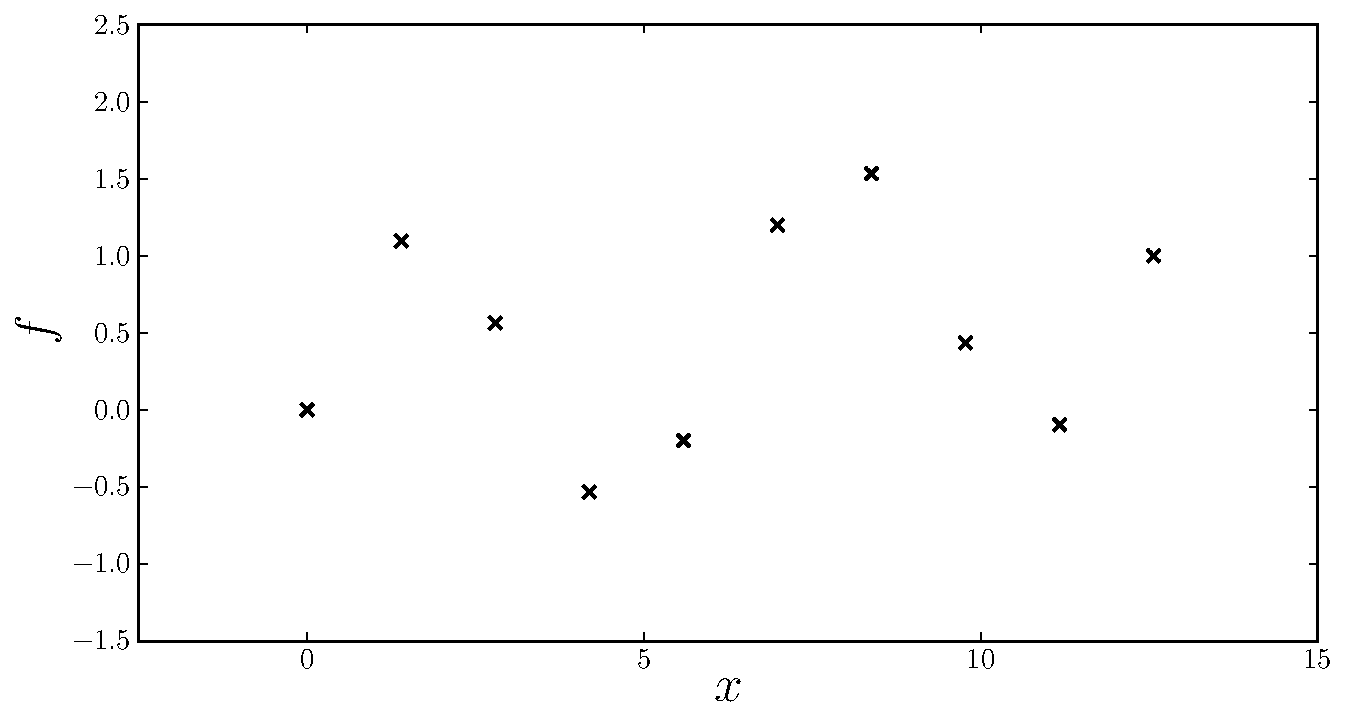
\includegraphics[height=5cm]{1_stat_models/figures/R/Fig1-data}
\end{center}
The vector of observations is $F=f(X)$ (ie $F_i = f(X_i)$ ).
\end{frame}

%%%%%%%%%%%%%%%%%%%%%%%%%%%%%%%%%%%%%%%%%%%%%%%%%%%%%%
\begin{frame}{}
Since $f$ in unknown, we make the general assumption that
it is the sample path of a Gaussian process $Z \sim \mathcal{N}(0,k)$:
\begin{center}
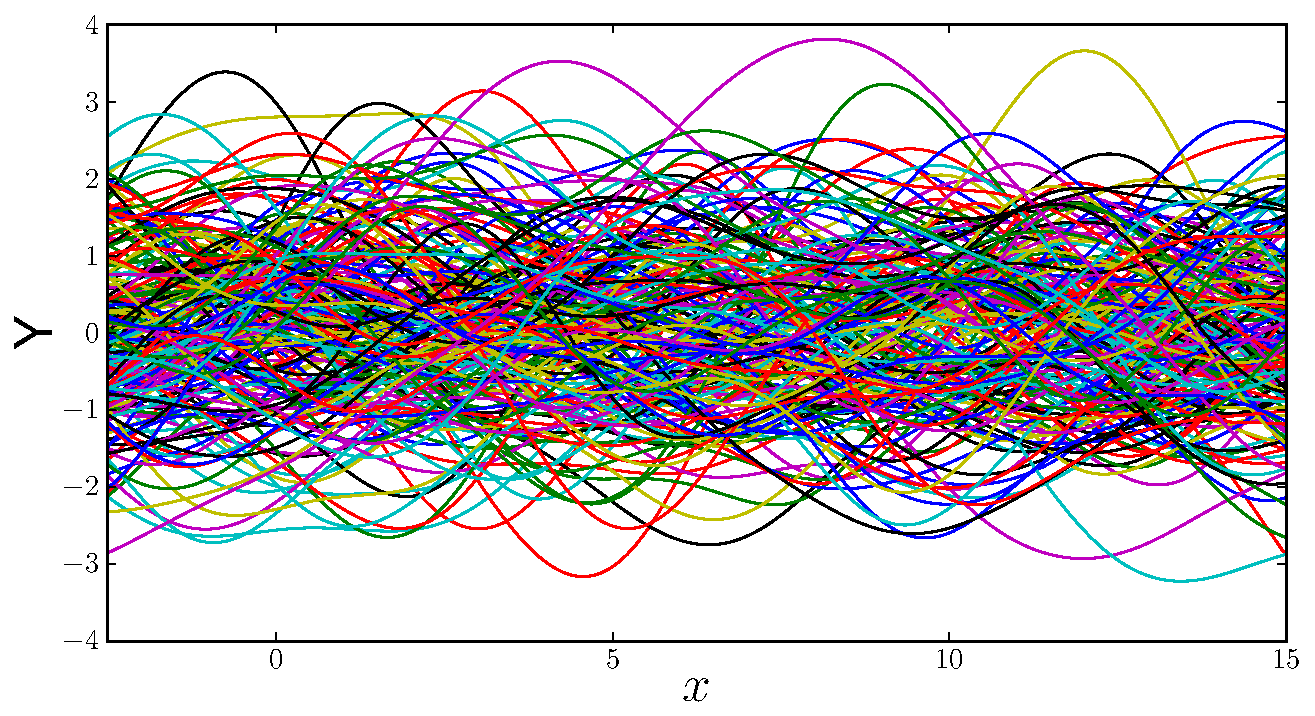
\includegraphics[height=5cm]{1_stat_models/figures/R/Fig1b-sim}
\end{center}
What would be the next step?
\end{frame}

%%%%%%%%%%%%%%%%%%%%%%%%%%%%%%%%%%%%%%%%%%%%%%%%%%%%%%
\begin{frame}{}
If we remove all the samples that do not interpolate we obtain:
\begin{center}
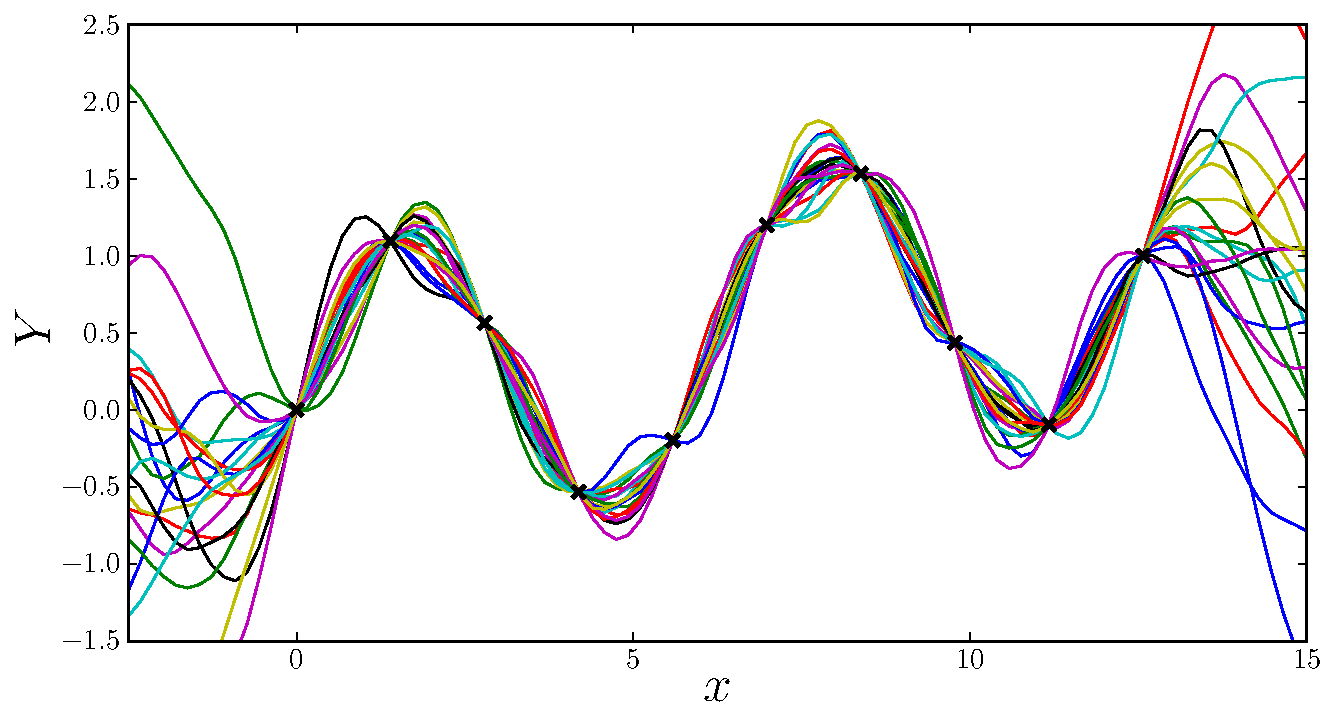
\includegraphics[height=6cm]{1_stat_models/figures/R/Fig1-sim-cond}
\end{center}
\end{frame}

%%%%%%%%%%%%%%%%%%%%%%%%%%%%%%%%%%%%%%%%%%%%%%%%%%%%%%
\begin{frame}{}
It can summarized by a mean function and 95\% confidence intervals.
\begin{center}
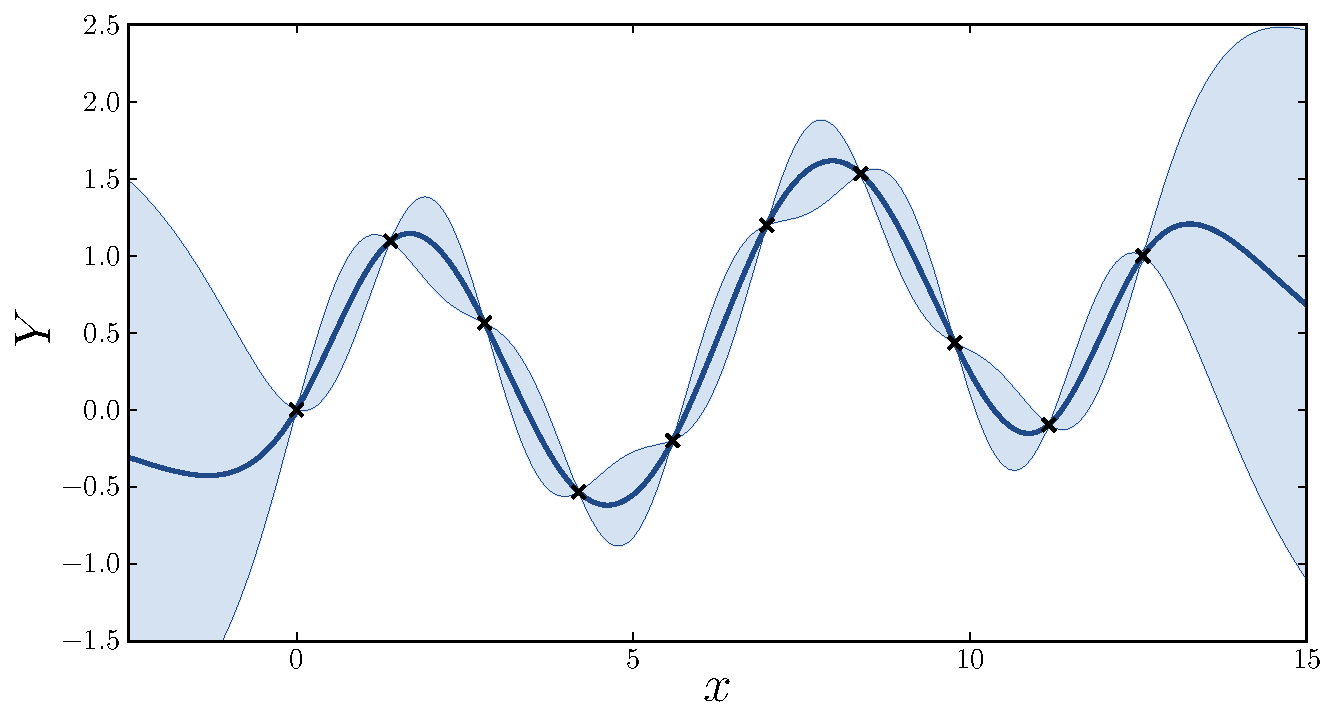
\includegraphics[height=6cm]{1_stat_models/figures/R/Fig1-GP}
\end{center}
\end{frame}

%%%%%%%%%%%%%%%%%%%%%%%%%%%%%%%%%%%%%%%%%%%%%%%%%%%%%%
\begin{frame}{}
In practice, the conditional distribution can be obtained analyticaly:\\
\vspace{5mm}
By definition, $(Z(x),Z(X))$ is multivariate normal so we know the distribution of $Z(x)|Z(X)=F$ is $\mathcal{N}(m(.),c(.,.))$ with:
\begin{equation*}
\begin{split}
    m(x) &= \E[Z(x)|Z(X) \shorteq F] \\
    &= k(x,X) k(X,X)^{-1} F \\ \vspace{3mm}
    c(x,y) &= \Cov[Z(x),Z(y)|Z(X) \shorteq F] \\
    &= k(x,y) - k(x,X) k(X,X)^{-1} k(X,y)
\end{split}
\end{equation*}
\end{frame}

%%%%%%%%%%%%%%%%%%%%%%%%%%%%%%%%%%%%%%%%%%%%%%%%%%%%%%
\begin{frame}{}
A few remarkable properties of GPR models
\begin{itemize}
	\item They (can) interpolate the data-points
	\item The prediction variance does not depend on the observations
	\item The mean predictor does not depend on the variance parameter
	\item They (usually) come back to zero when we are far away from the observations.
\end{itemize}
Can we prove them?
\end{frame}


%%%%%%%%%%%%%%%%%%%%%%%%%%%%%%%%%%%%%%%%%%%%%%%%%%%%%%
\begin{frame}{}
Changing the kernel \alert{has a huge impact on the model}:\\
\vspace{5mm}
\begin{center}
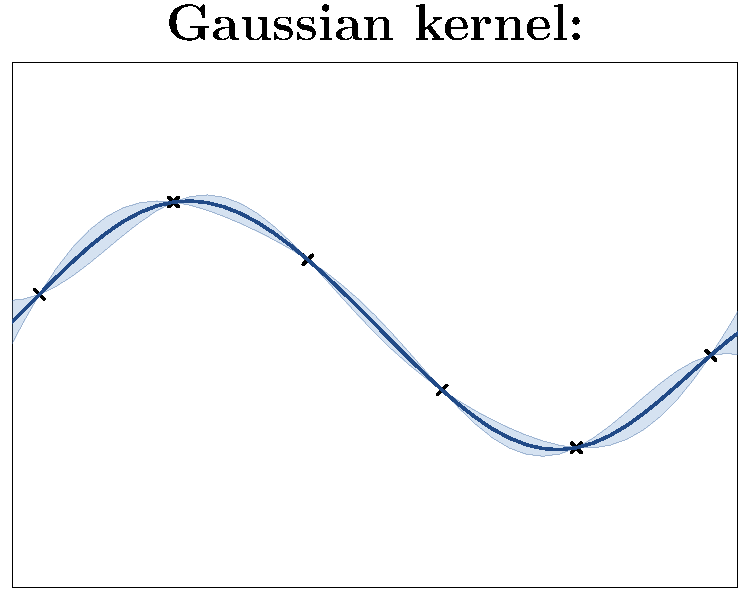
\includegraphics[height=3.9cm]{1_stat_models/figures/Fig2-GP-rbf} \qquad
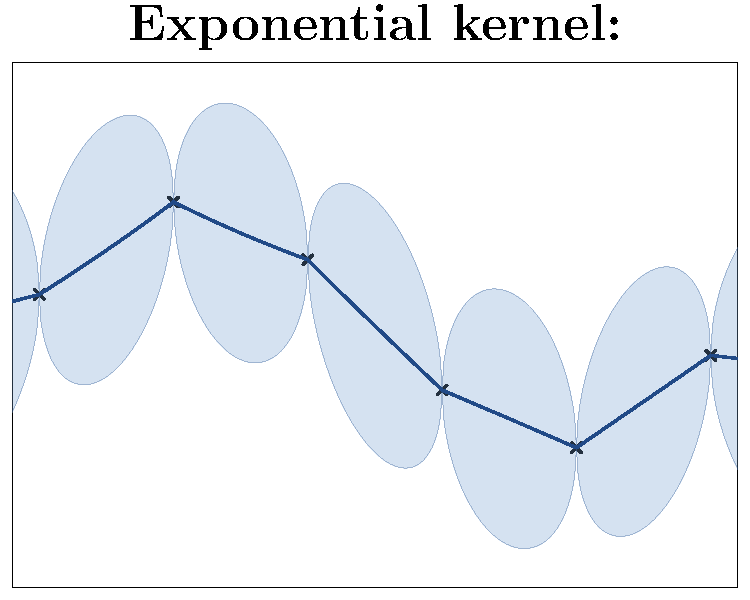
\includegraphics[height=3.9cm]{1_stat_models/figures/Fig2-GP-exp}
\end{center}
\end{frame}

%%%%%%%%%%%%%%%%%%%%%%%%%%%%%%%%%%%%%%%%%%%%%%%%%%%%%%
\begin{frame}{}
This is because changing the kernel means changing the prior on $f$\\
\vspace{5mm}
\begin{center}
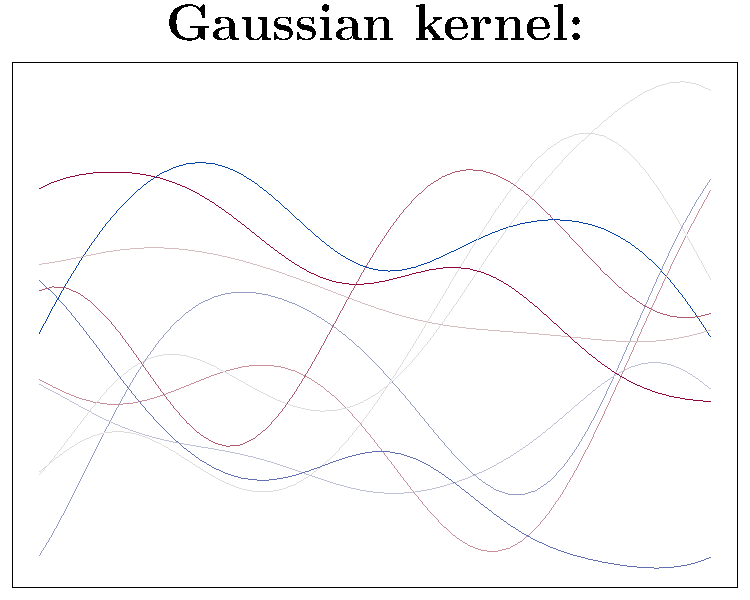
\includegraphics[height=3.8cm]{1_stat_models/figures/Fig2-sim-rbf} \qquad
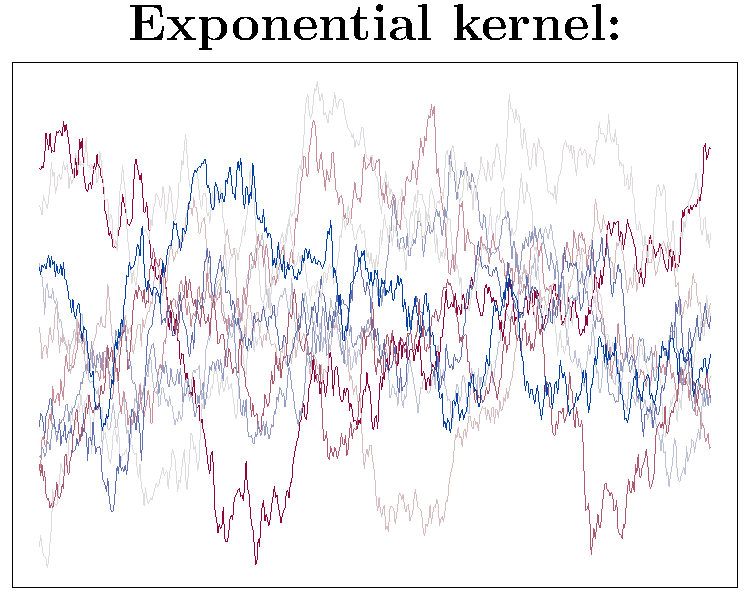
\includegraphics[height=3.8cm]{1_stat_models/figures/Fig2-sim-exp}
\end{center}
\end{frame}

%%%%%%%%%%%%%%%%%%%%%%%%%%%%%%%%%%%%%%%%%%%%%%%%%%%%%%
\begin{frame}{}
There is no kernel that is intrinsically better... it depends on data!
\begin{center}
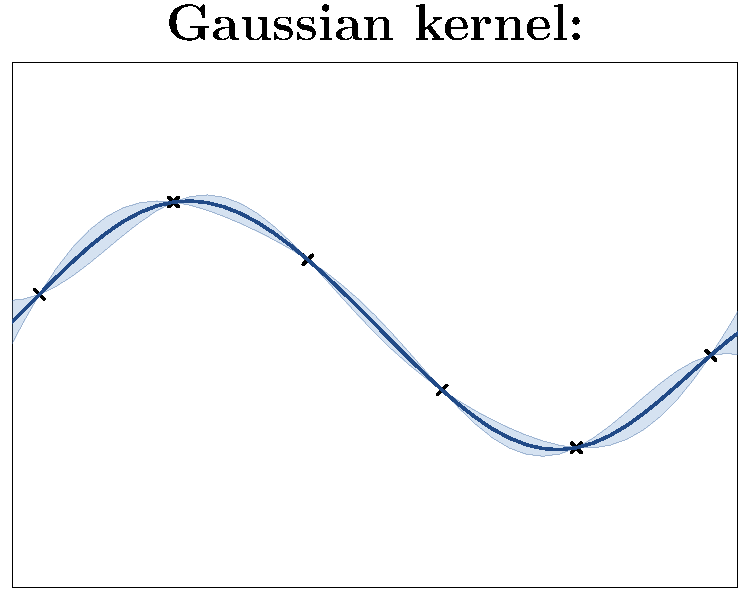
\includegraphics[height=3.5cm]{1_stat_models/figures/Fig2-GP-rbf} \hspace{1cm}
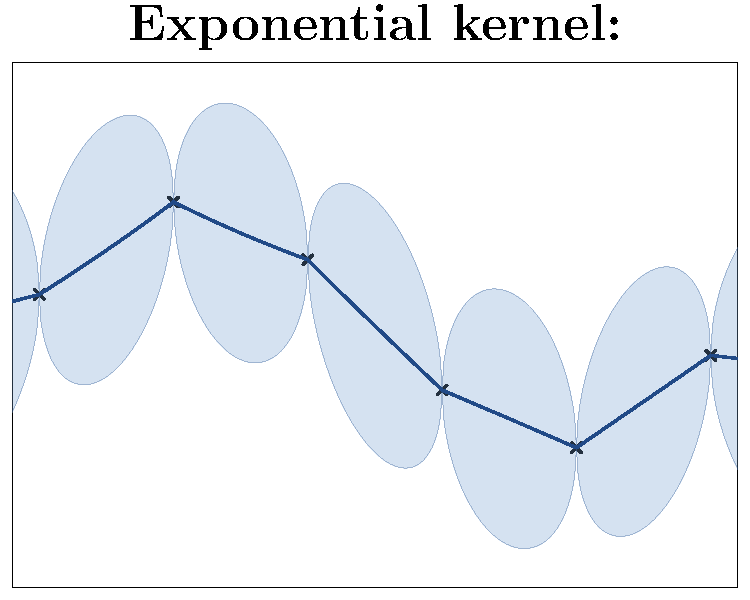
\includegraphics[height=3.5cm]{1_stat_models/figures/Fig2-GP-exp}
\end{center}
The kernel has to be chosen accordingly to our prior belief on the behaviour of the function to study:
\begin{itemize}
  \item is it continuous, differentiable, how many times?
  \item is it stationary ?
  \item ...
\end{itemize}
\end{frame}

%%%%%%%%%%%%%%%%%%%%%%%%%%%%%%%%%%%%%%%%%%%%%%%%%%%%%%
\begin{frame}{}
\begin{exampleblock}{Example}
Let's recreate the map of displacements using a subset of the data    
\begin{center}
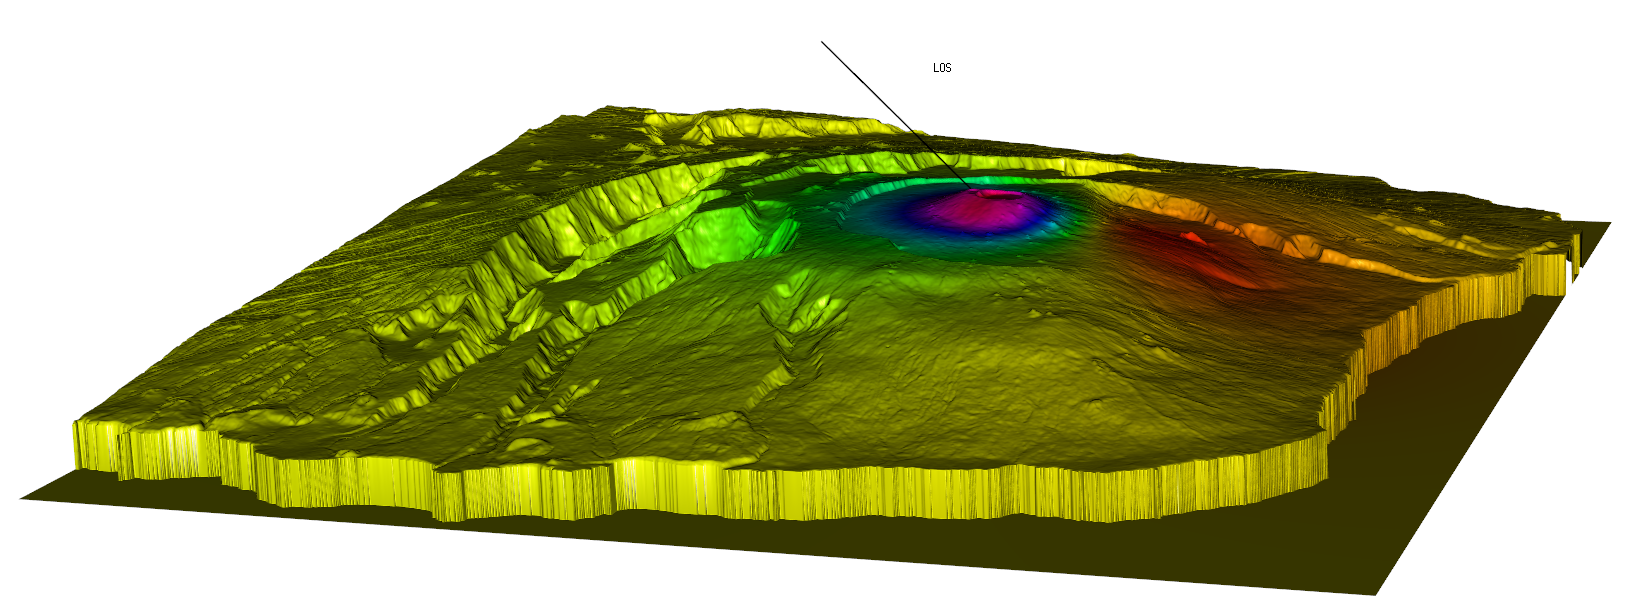
\includegraphics[height=4cm]{1_stat_models/figures/piton_ulos_2}
\end{center}
\end{exampleblock}
\alert{$\Rightarrow$ R demo}
\end{frame}

%%%%%%%%%%%%%%%%%%%%%%%%%%%%%%%%%%%%%%%%%%%%%%%%%%%%%%
\begin{frame}{}
We are not always interested in models that interpolate the data. For example, if there is some observation noise: $F = f(X) + \varepsilon$.
\vspace{5mm}
Let $N$ be a process $\mathcal{N}(0,n(.,.))$ that represent the observation noise. The expressions of GPR with noise are
\begin{equation*}
	\begin{split}
	m(x) &= \E[Z(x)|Z(X) + N(X) \shorteq F] \\
	&= k(x,X) (k(X,X)+n(X,X))^{-1} F \\
	& \\
	c(x,y) &= \Cov[Z(x),Z(y)|Z(X)+ N(X) \shorteq F] \\
	&= k(x,y) - k(x,X) (k(X,X)+n(X,X))^{-1} k(X,y)
\end{split}
\end{equation*}
\end{frame}

%%%%%%%%%%%%%%%%%%%%%%%%%%%%%%%%%%%%%%%%%%%%%%%%%%%%%%
\begin{frame}{}
Examples of models with observation noise for $n(x,y)=\tau^2 \delta_{x,y}$:
\begin{center}
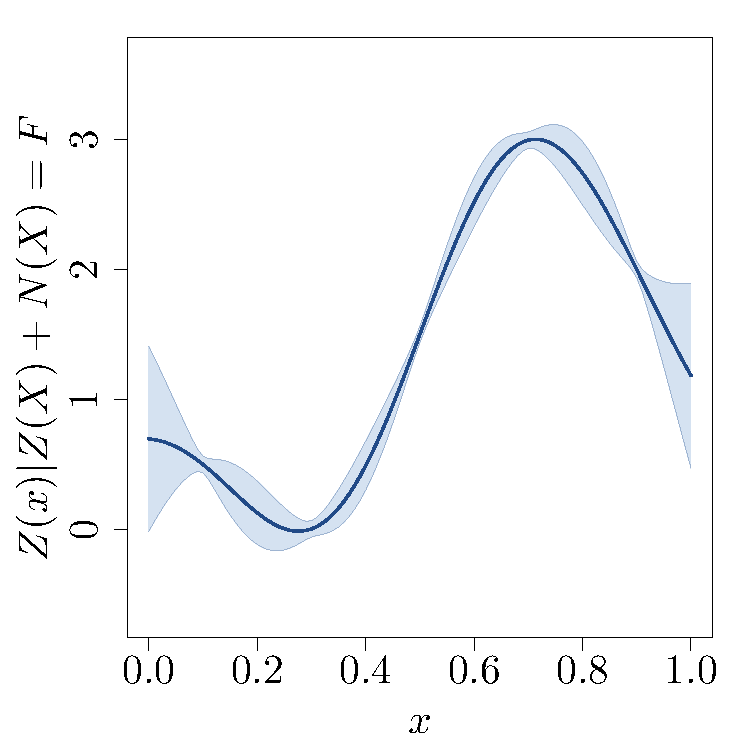
\includegraphics[height=3.5cm]{1_stat_models/figures/R/ch34_GPRnoise0001}
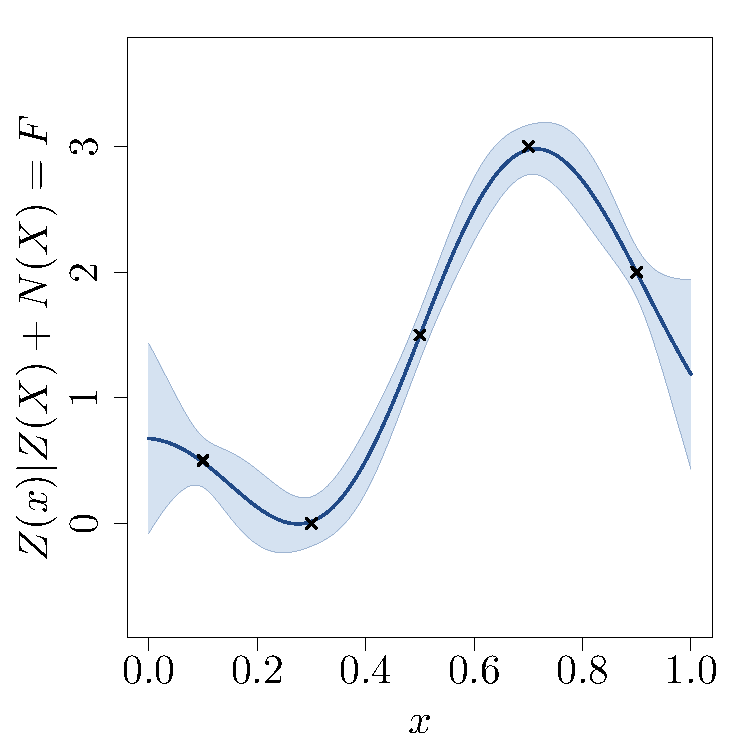
\includegraphics[height=3.5cm]{1_stat_models/figures/R/ch34_GPRnoise001}
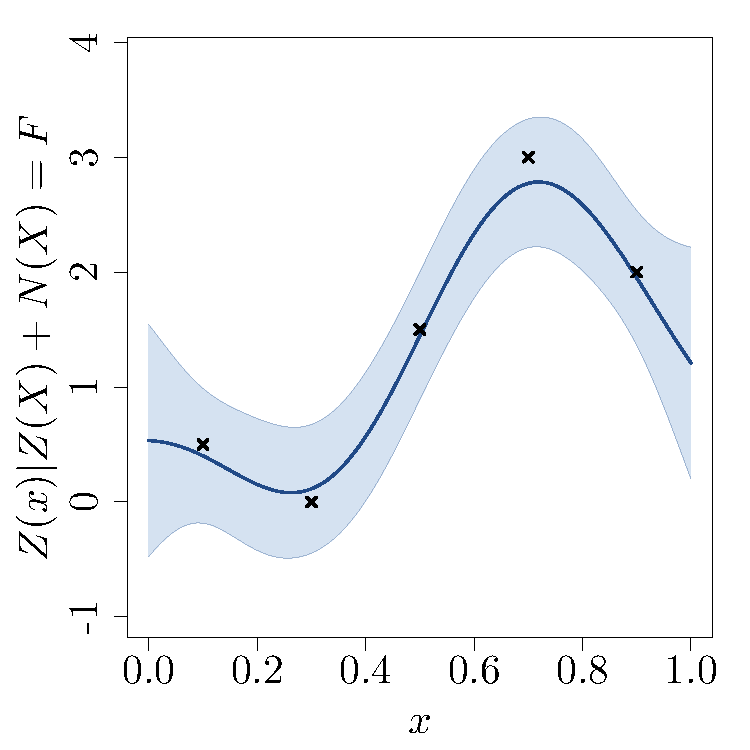
\includegraphics[height=3.5cm]{1_stat_models/figures/R/ch34_GPRnoise01}\\
The values of $\tau^2$ are respectively 0.001, 0.01 and 0.1.
\end{center}
\end{frame}


%%%%%%%%%%%%%%%%%%%%%%%%%%%%%%%%%%%%%%%%%%%%%%%%%%%%%%%
%%%%%%%%%%%%%%%%%%%%%%%%%%%%%%%%%%%%%%%%%%%%%%%%%%%%%%
\section[DoE]{Design of experiments}
\subsection{}


%%%%%%%%%%%%%%%%%%%%%%%%%%%%%%%%%%%%%%%%%%%%%%%%%%%%%%
\begin{frame}{}
We have seen yesterday how to build a model from a given set of input/output tuples:
\begin{center}
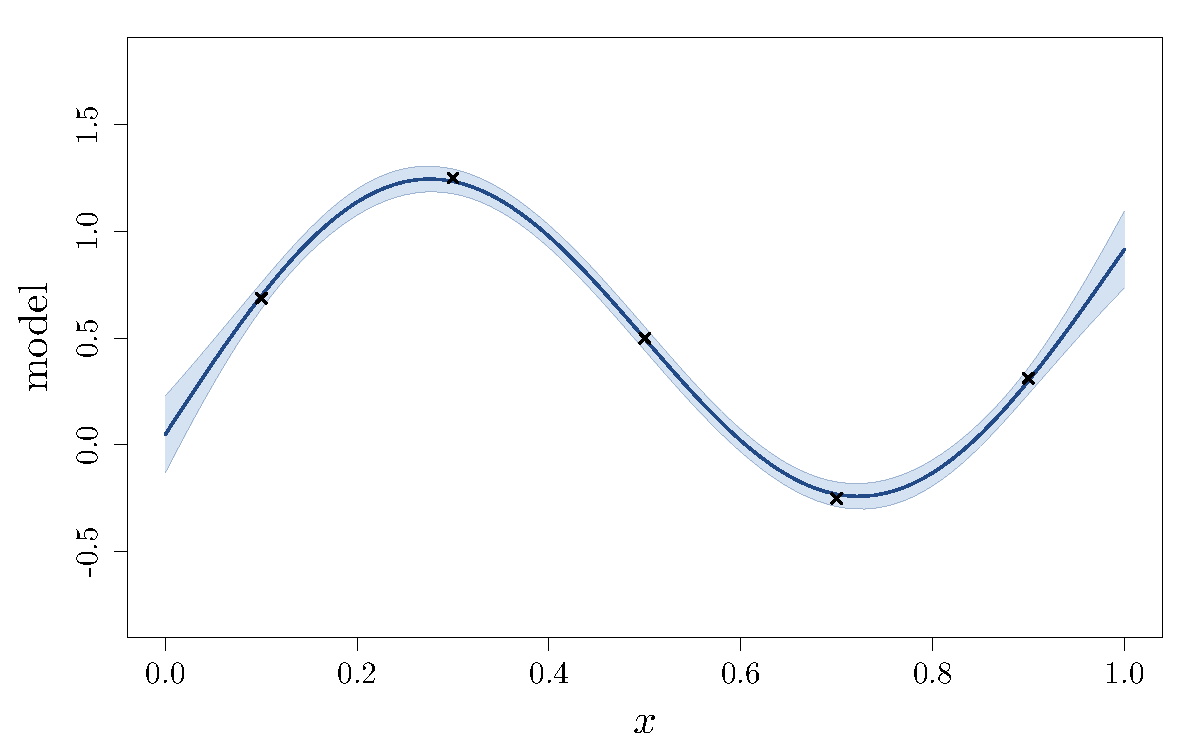
\includegraphics[height=5cm]{2_Design_of_experiments/figures/R/model_0}
\end{center}
Today's question is: How to choose the input points to get the best model?
\end{frame}

%%%%%%%%%%%%%%%%%%%%%%%%%%%%%%%%%%%%%%%%%%%%%%%%%%%%%%
\begin{frame}{}
\begin{exampleblock}{Motivating example}
Same number of points but different input locations \vspace{-2mm}
\begin{center}
  \begin{tabular}{cc}
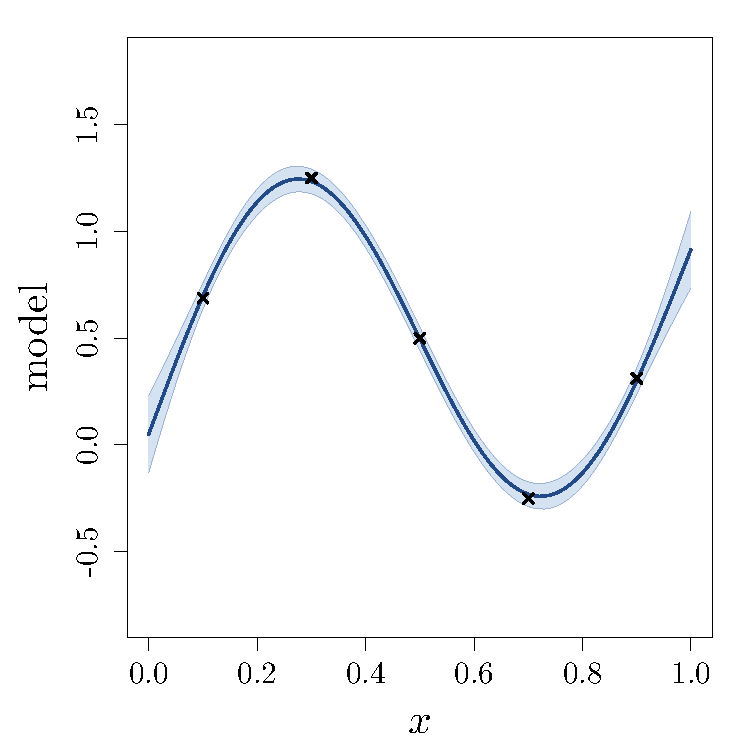
\includegraphics[height=5cm]{2_Design_of_experiments/figures/R/model_1} & 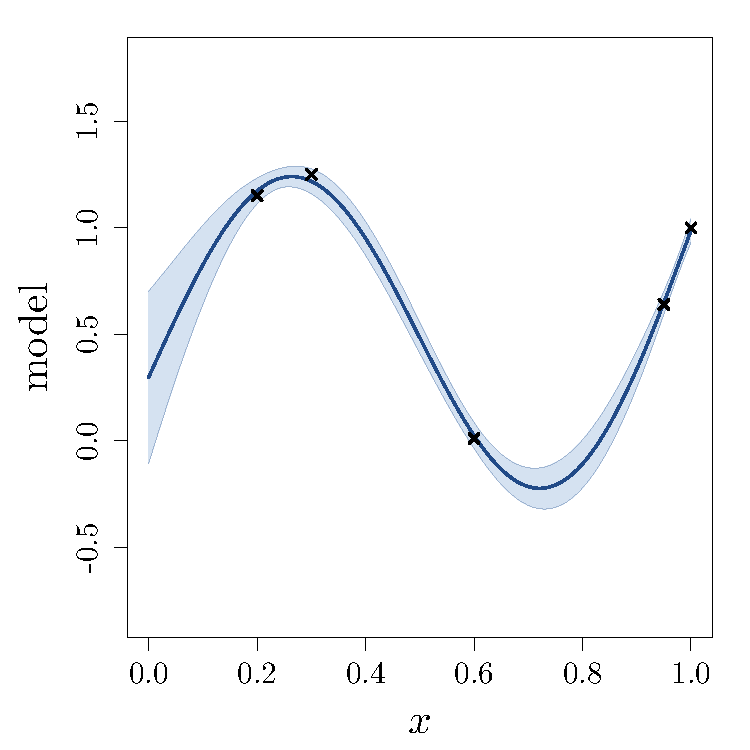
\includegraphics[height=5cm]{2_Design_of_experiments/figures/R/model_2} \\
$RSS = 0.054$ & $RSS = 0.68$ \\
$IMSE = 0.001$ & $IMSE = 0.004$
  \end{tabular}
\end{center}
\end{exampleblock}
\end{frame}

%%%%%%%%%%%%%%%%%%%%%%%%%%%%%%%%%%%%%%%%%%%%%%%%%%%%%%
\begin{frame}{}
\structure{Outline of the lecture}
\vspace{0.2cm}
\begin{itemize}
	\item Classical designs
	\item Space filling designs
	\item Optimal design for a given model
\end{itemize}
\vspace{5mm}
This lecture is based on a course of Victor Picheny (INRA) at Mines St-\'Etienne.\\
\vspace{5mm}
We have focus in the past lecture on 1-dimensional examples, we have to bear in mind that the input space is often of high dimension ($d$ from 5 to 100).
\end{frame}

%%%%%%%%%%%%%%%%%%%%%%%%%%%%%%%%%%%%%%%%%%%%%%%%%%%%%%
\begin{frame}{}
Intuition is often misleading in high-dimension:
\begin{exampleblock}{Examples 1/2}
\begin{itemize}
	\item Points in the unit cube can be far away\\ \qquad $\rightarrow$ the diagonal of the unit cube is of length $\sqrt{d}$
	\item All the volume is near the domain boundaries \\ \qquad $\rightarrow$ let us consider a hypercube of size 0.9 included in the the unit cube:\vspace{5mm}
	\begin{center}
\includegraphics[height=4cm]{2_Design_of_experiments/figures/latexdraw/volumedim} \quad
\includegraphics[height=3.5cm]{2_Design_of_experiments/figures/python/spf_volume}
\end{center}
\end{itemize}
\end{exampleblock}
\end{frame}

%%%%%%%%%%%%%%%%%%%%%%%%%%%%%%%%%%%%%%%%%%%%%%%%%%%%%%
\begin{frame}{}
Intuition is often misleading in high-dimension:
\begin{exampleblock}{Examples 2/2}
\begin{itemize}
	\item The number of vertices of an hypercube increases faster than we usually think
\end{itemize}
\begin{columns}[c]
\column{5.5cm}
\includegraphics[height=4.5cm]{2_Design_of_experiments/figures/crashtest}
\column{5cm}
Testing all combinations of min and max input values for the 50 parameters would require... \pause \\

\textbf{3000 times the age of the universe}!\\
($d=50$ $\rightarrow$ $2^d \approx 1.e15$)
\end{columns}
\end{exampleblock}
\end{frame}

%%%%%%%%%%%%%%%%%%%%%%%%%%%%%%%%%%%%%%%%%%%%%%%%%%%%%%
%%%%%%%%%%%%%%%%%%%%%%%%%%%%%%%%%%%%%%%%%%%%%%%%%%%%%%
\section[Classical DoE]{Classical designs}
\subsection{}

%%%%%%%%%%%%%%%%%%%%%%%%%%%%%%%%%%%%%%%%%%%%%%%%%%%%%%
\begin{frame}{One at a time design}
An intuitive way to check the influence of various variable is to make them change one at the time.
\begin{itemize}
	\item All variables are fixed at a reference value (0 for example)
	\item One variable is changed at a time to see if there is an influence
\end{itemize}
\vspace{5mm}
\begin{example}
\begin{columns}[c]
\column{5cm}
\begin{center}
\includegraphics[width=4cm]{2_Design_of_experiments/figures/latexdraw/1atatime}
\end{center}
\column{5cm}
\begin{center}
  \begin{tabular}{|c|ccc|}
  \hline
  point & $x_1$ & $x_2$ & $x_3$ \\ \hline
  $X_1$ & 0 & 0 & 0 \\
  $X_2$ & 1 & 0 & 0 \\
  $X_3$ & 0 & 1 & 0 \\
  $X_4$ & 0 & 0 & 1 \\ \hline
  \end{tabular}
\end{center}
\end{columns}
\end{example}
\end{frame}

%%%%%%%%%%%%%%%%%%%%%%%%%%%%%%%%%%%%%%%%%%%%%%%%%%%%%%
\begin{frame}{}
\textbf{pros and cons of this kind of design}:
\begin{itemize}
  \item[+] require only $d+1$ observations
  \item[+] are easy to interpret
  \item[] \vspace{-4mm}
  \item[$-$] they can only see linear effects:
  \begin{center}
  $m(x)=\beta_0 + \beta_1 x_1 + \beta_2 x_2 + \beta_3 x_3$
  \end{center}
  \item[$-$] they do not cover the space
\end{itemize}
\vspace{5mm}
\begin{exampleblock}{Exercise}
How can this kind of design be adapted to estimate quadratic effect?
\end{exampleblock}
\end{frame}

%%%%%%%%%%%%%%%%%%%%%%%%%%%%%%%%%%%%%%%%%%%%%%%%%%%%%%
\begin{frame}{}
\begin{exampleblock}{Solution}
Quadratic effects can be estimated with either
\begin{center}
\includegraphics[width=4.5cm]{2_Design_of_experiments/figures/latexdraw/1atatime1} \hspace{10mm}
\includegraphics[width=4.5cm]{2_Design_of_experiments/figures/latexdraw/1atatime2}
\end{center}
we sometime talk about ``star shaped'' design.
\end{exampleblock}
\end{frame}

%%%%%%%%%%%%%%%%%%%%%%%%%%%%%%%%%%%%%%%%%%%%%%%%%%%%%%
\begin{frame}{Factorial designs}
The principle of factorial design is to consider all combinations for $x_i \in \{0,1\}$:
\vspace{5mm}
\begin{columns}[c]
\column{4cm}
\begin{center}
\includegraphics[width=4cm]{2_Design_of_experiments/figures/latexdraw/factorial}
\end{center}
\column{6cm}
\begin{itemize}
	\item[\textbf{pros}] They allow to get all interaction terms:
\end{itemize}
	$$\beta_0 + \sum_k \beta_k x_k + \sum_{j,k} \beta_{j,k} x_j x_k  + \beta_{1,2,3} x_1 x_2 x_3$$
\begin{itemize}
	\item[\textbf{cons}] The number of evaluation is unrealistic when $d$ is large
\end{itemize}
\end{columns}
\end{frame}

%%%%%%%%%%%%%%%%%%%%%%%%%%%%%%%%%%%%%%%%%%%%%%%%%%%%%%
\begin{frame}{Factorial designs}
It is also possible to build factorial designs with $k$ levels:
\begin{center}
\includegraphics[width=5cm]{2_Design_of_experiments/figures/latexdraw/factorial3levels}
\end{center}
This allows to compute quadratic effects but the number of evaluations $k^d$ is even less realistic...
\end{frame}

%%%%%%%%%%%%%%%%%%%%%%%%%%%%%%%%%%%%%%%%%%%%%%%%%%%%%%
\begin{frame}{}
\textbf{Conclusion on classical designs:}\\
\structure{\textbf{pros:}}\\
\quad Easy to use\\
\quad adapted to continuous or discrete variables\\
\quad Can be combined (star + factorial for example)\\
\quad Well suited (often optimal) for linear regression\\
\vspace{5mm}
\structure{\textbf{cons:}}\\
\quad Number of evaluation is not flexible\\
\quad Number of evaluation too large in high dimension\\
\quad Points are on top of each other when projected
\end{frame}

%%%%%%%%%%%%%%%%%%%%%%%%%%%%%%%%%%%%%%%%%%%%%%%%%%%%%%
\begin{frame}{projection issues}
Why don't we want points to be superimposed when projected?\\
If one of the variables has no influence, most observations become redundant...
\begin{center}
\includegraphics[height=4.5cm]{2_Design_of_experiments/figures/latexdraw/factorialprojection}
\end{center}
From 27 observations, we end up with only 9...
\end{frame}

%%%%%%%%%%%%%%%%%%%%%%%%%%%%%%%%%%%%%%%%%%%%%%%%%%%%%%
%%%%%%%%%%%%%%%%%%%%%%%%%%%%%%%%%%%%%%%%%%%%%%%%%%%%%%
\section{Space filling DoE}
\subsection{}


%%%%%%%%%%%%%%%%%%%%%%%%%%%%%%%%%%%%%%%%%%%%%%%%%%%%%%
\begin{frame}{}
We will now focus on designs of experiments that:
\begin{itemize}
	\item are not model oriented
	\item give information about every domain of the input space
	\item have good projection on subspaces
	\item have a flexible number of points
\end{itemize}
\end{frame}

%%%%%%%%%%%%%%%%%%%%%%%%%%%%%%%%%%%%%%%%%%%%%%%%%%%%%%
\begin{frame}{}
How can we evaluate if a set of points fills the space?\\ \vspace{5mm}
\textbf{Option 1.} Compute distances between points\\
\begin{itemize}
	\item[maximin] the minimum distance between two points of the design should be large:
	$$\text{Optimisation problem is: \quad} \max_{X_1,\dots,X_n} [ \min_{i \neq j} dist(X_i,X_j) ]$$
	\item[minimax] the maximum distance between any point of the space and closest design point should be small:
	$$\text{Optimisation problem is: \quad} \min_{X_1,\dots,X_n} (\max_{x \in D} [ \min_i dist(x,X_i) ])$$
\end{itemize}
The second criterion is much more difficult to optimise
\end{frame}

%%%%%%%%%%%%%%%%%%%%%%%%%%%%%%%%%%%%%%%%%%%%%%%%%%%%%%
\begin{frame}{}
These criteria can be illustrated on a simple 2-dimensional example
\begin{center}
\includegraphics[height=6.5cm]{2_Design_of_experiments/figures/python/spf_minimaxmaximin}
\end{center}
\end{frame}

%%%%%%%%%%%%%%%%%%%%%%%%%%%%%%%%%%%%%%%%%%%%%%%%%%%%%%
\begin{frame}{}
How can we evaluate if a set of points fills the space?\\ \vspace{2mm}
\textbf{Option 2.} Compare the distribution with an uniform distribution\\ \vspace{2mm}
\structure{Discrepency} is a measure of non uniformity. It compares the number of points in a hyper-rectangle with the expected number of samples from a uniform distribution
\vspace{-2mm}
\begin{columns}[c]
\column{4cm}
\begin{center}
\includegraphics[height=4cm]{2_Design_of_experiments/figures/latexdraw/discrepency}
\end{center}
\column{6cm}
\vspace{1mm}
The probability for a uniform variable to be in $R$ is 0.22 and we observe an empirical probability of $2/11$. The discrepancy (w.r.t. $R$) is then:
$$D_R = |0.22-2/11| = 0.038$$
\end{columns}
\vspace{2mm}
Discrepency is defined as the sup of the distance between the empirical and analytical cdf.
\end{frame}

%%%%%%%%%%%%%%%%%%%%%%%%%%%%%%%%%%%%%%%%%%%%%%%%%%%%%%
\begin{frame}{}
Discrepency is often computed by:
\begin{itemize}
 	\item fixing one of the hyper-rectangle summit at the origin
 	\item centering the hyper-rectangle
 \end{itemize}
\begin{center}
\includegraphics[height=4.5cm]{2_Design_of_experiments/figures/latexdraw/discrepency3}
\end{center}
The maximum is located where the rectangle is tangent to points\\
$\rightarrow$ The optimisation is over a finite space
\end{frame}

%%%%%%%%%%%%%%%%%%%%%%%%%%%%%%%%%%%%%%%%%%%%%%%%%%%%%%
\begin{frame}{}
We will now give an overview on three types of space filling designs:
\begin{itemize}
	\item Latin hypercubes
	\item low discrepancy sequences
	\item centroidal Voronoi tesselations
\end{itemize}
\end{frame}

%%%%%%%%%%%%%%%%%%%%%%%%%%%%%%%%%%%%%%%%%%%%%%%%%%%%%%
\begin{frame}{Latin hypercubes}
\textbf{Latin hypercubes} are designs where the domain is sliced in $n^d$ blocks and where there is only one point per ``line'' and ``column'':
\begin{center}
\includegraphics[height=5cm]{2_Design_of_experiments/figures/latexdraw/lhs1}
\end{center}
These designs have good projection properties
\end{frame}


%%%%%%%%%%%%%%%%%%%%%%%%%%%%%%%%%%%%%%%%%%%%%%%%%%%%%%
\begin{frame}{}
A well known example of LHS in 2D is... Sudoku
\vspace{5mm}
\begin{center}
\includegraphics[height=5cm]{2_Design_of_experiments/figures/sudoku}
\end{center}
\end{frame}

%%%%%%%%%%%%%%%%%%%%%%%%%%%%%%%%%%%%%%%%%%%%%%%%%%%%%%
\begin{frame}{}
If we focus on one digit (say $4$), we obtain a LHD:
\vspace{2mm}
\begin{center}
\includegraphics[height=5cm]{2_Design_of_experiments/figures/latexdraw/sudoku}
\end{center}
Sudoku have more properties that LHD: the generalisation is called \textbf{orthogonal array}.
\end{frame}

%%%%%%%%%%%%%%%%%%%%%%%%%%%%%%%%%%%%%%%%%%%%%%%%%%%%%%
\begin{frame}{}
Latin hypercubes do not necessarily cover the space very well...
\begin{center}
\includegraphics[height=4.5cm]{2_Design_of_experiments/figures/latexdraw/lhs2}
\end{center}
They have to be combined with a criterion such as maximin.
\end{frame}

%%%%%%%%%%%%%%%%%%%%%%%%%%%%%%%%%%%%%%%%%%%%%%%%%%%%%%
\begin{frame}{}
\begin{exampleblock}{Exercise}
\begin{itemize}
	\item Generate a 5 points LHD in dimension 3.
	\item How would you program a function \texttt{LHD(n,d)}?
	\item How would you optimize a LHD to ensure it fills the space properly?
\end{itemize}
\end{exampleblock}
\end{frame}

%%%%%%%%%%%%%%%%%%%%%%%%%%%%%%%%%%%%%%%%%%%%%%%%%%%%%%
\begin{frame}{}
\begin{exampleblock}{Solution}
The coordinates of two points can be exchanged:\\
\vspace{4mm}
\begin{center}
\includegraphics[height=4.5cm]{2_Design_of_experiments/figures/latexdraw/lhs3}
\end{center}
\end{exampleblock}
\end{frame}

%%%%%%%%%%%%%%%%%%%%%%%%%%%%%%%%%%%%%%%%%%%%%%%%%%%%%%
\begin{frame}{}
LHD optimization with simulated annealing:\\
\vspace{4mm}
\textbf{Morris and Mitchell Algorithm}\\
\vspace{2mm}
\begin{itemize}
	\item[1] Generate LHD
	\item[2] find ``bad'' points according to maximin
	\item[3] choose randomly a column of this critical point and exchange it with an randomly selected other point
	\item[4] \qquad if the criteria is improved, the modification is accepted
	\item[5] \qquad otherwise, it is accepted with a probability of $$\exp \left(\frac{maximin_{new}-maximin_{old}}{T}\right)$$
	\end{itemize}
\end{frame}



%%%%%%%%%%%%%%%%%%%%%%%%%%%%%%%%%%%%%%%%%%%%%%%%%%%%%%
\begin{frame}{Low discrepancy sequences}
\textbf{Low discrepancy sequences} are deterministic sequences that converge toward the uniform distribution.
\begin{itemize}
	\item They cover the space quickly and evenly
	\item They are easy to build
	\item It is easy to add new points
\end{itemize}
\vspace{5mm}
Many low discrepancy sequences can be found in the literature: Halton, Hammerley, Sobol', Faure, van der Corput, ...
\end{frame}

%%%%%%%%%%%%%%%%%%%%%%%%%%%%%%%%%%%%%%%%%%%%%%%%%%%%%%
\begin{frame}{}
\begin{example}[Halton sequence]
	Let $a$ and $b$ be two integers with no common dividers (say 2 and 3). The $x_1$ and $x_2$ coordinates of the Halton sequence are:
	\begin{equation*}
		\begin{split}
			x_1 &= 1/2,\ 1/4,\ 3/4,\ 1/8,\ 5/8,\ 3/8,\ 7/8,\ 1/16,\ 9/16, \dots\\
			x_2 &= 1/3,\ 2/3,\ 1/9,\ 4/9,\ 7/9,\ 2/9,\ 5/9,\ 8/9,\ 1/27, \dots
		\end{split}
	\end{equation*}
\begin{center}
\includegraphics[height=4.5cm]{2_Design_of_experiments/figures/python/spf_halton}
\end{center}

\end{example}
\end{frame}

%%%%%%%%%%%%%%%%%%%%%%%%%%%%%%%%%%%%%%%%%%%%%%%%%%%%%%
\begin{frame}{}
\begin{example}[Halton sequence]
\begin{center}
  \begin{tabular}{cc}
Halton Sequence & uniform pseudo random \\
\includegraphics[height=5cm]{2_Design_of_experiments/figures/Halton} & \includegraphics[height=5cm]{2_Design_of_experiments/figures/random}
  \end{tabular}
 source: wikipedia
\end{center}
\end{example}
\end{frame}

%%%%%%%%%%%%%%%%%%%%%%%%%%%%%%%%%%%%%%%%%%%%%%%%%%%%%%
\begin{frame}{}
Issues with low discrepancy sequences:
\begin{itemize}
	\item[$-$] there can be alignments when projected
	\item[$-$] there can be holes in subspaces
	\item[$-$] points may be aligned (Example: 16 first points in basis (17,18))
\end{itemize}
\end{frame}

%%%%%%%%%%%%%%%%%%%%%%%%%%%%%%%%%%%%%%%%%%%%%%%%%%%%%%
\begin{frame}{Centroidal Voronoi Tesselations}
Given a set of generative points $X$, the \textbf{Voronoi Tesselations} (or Voronoi cells) associated to the point $X_i$ is the region of the space such that $X_i$ is the closest point from the set:
\begin{center}
\includegraphics[height=5cm]{2_Design_of_experiments/figures/VT}
\end{center}
Source: Q. Du et Al., \emph{Centroidal Voronoi Tessellations: Applications and Algorithms}, SIAM Review, 41-4, 1999.
\end{frame}

%%%%%%%%%%%%%%%%%%%%%%%%%%%%%%%%%%%%%%%%%%%%%%%%%%%%%%
\begin{frame}{}
\textbf{Centroidal Voronoi Tesselations (CVT)} is a special case of Voronoi Tesselations where the generative points correspond to the centre of mass of the cells
\begin{center}
\includegraphics[height=5cm]{2_Design_of_experiments/figures/CVT}
\end{center}
Source: Q. Du et Al., \emph{Centroidal Voronoi Tessellations: Applications and Algorithms}, SIAM Review, 41-4, 1999.
\end{frame}

%%%%%%%%%%%%%%%%%%%%%%%%%%%%%%%%%%%%%%%%%%%%%%%%%%%%%%
\begin{frame}{}

Properties of CVT:
\begin{itemize}
	\item Each point of the space is close to one generative points
	\item The generative points cover the space
\end{itemize}
$\Rightarrow$ The generative points of CVT can be used as design of experiment.
\end{frame}

%%%%%%%%%%%%%%%%%%%%%%%%%%%%%%%%%%%%%%%%%%%%%%%%%%%%%%
\begin{frame}{Generating CVT }
\textbf{1. Lloyd's Algorithm}
\begin{itemize}
	\item[1] Initialize $X$ as a set of $n$ points
	\item[2] While $i<nb\_iter$
	\item[3] \qquad Compute the Voronoi diagram of $X$
	\item[4] \qquad X = centre of mass of each cell
\end{itemize}
\begin{center}
  \begin{tabular}{cccc}
\includegraphics[height=2.4cm]{2_Design_of_experiments/figures/Lloyds1}&
\includegraphics[height=2.4cm]{2_Design_of_experiments/figures/Lloyds2}&
\includegraphics[height=2.4cm]{2_Design_of_experiments/figures/Lloyds3}&
\includegraphics[height=2.4cm]{2_Design_of_experiments/figures/Lloyds15}\\
iteration 1 & iteration 2 &iteration 3 &iteration 15
  \end{tabular}
\end{center}
source: ``Lloyd's algorithm'' wikipedia page
\end{frame}

%%%%%%%%%%%%%%%%%%%%%%%%%%%%%%%%%%%%%%%%%%%%%%%%%%%%%%
\begin{frame}{Generating CVT }
\textbf{2. k-means}\\
This algorithm is very similar to Lloyd but it uses a large set of points covering the input space instead of the full continuous domain:
\begin{center}
\includegraphics[height=4.5cm]{2_Design_of_experiments/figures/python/spf_kmeans1}
\includegraphics[height=4.5cm]{2_Design_of_experiments/figures/Rightarrow}
\includegraphics[height=4.5cm]{2_Design_of_experiments/figures/python/spf_kmeans2}
\end{center}
\end{frame}

%%%%%%%%%%%%%%%%%%%%%%%%%%%%%%%%%%%%%%%%%%%%%%%%%%%%%%
\begin{frame}{Generating CVT }
\textbf{3. McQueen algorithm}\\
\vspace{5mm}
This algorithm is much faster than the previous ones and gives a good approximation
\begin{itemize}
	\item[1] Initialize $X$ as a set of $n$ points
	\item[2] Initialize $k$ as a vector of 1 with length $n$
	\item[3] While $i<nb\_iter$
	\item[4] \qquad generate one random point $z$ in the input space
	\item[5] \qquad find the $X_i$ closest to $z$
	\item[6] \qquad update $X_i = \frac{k_i X_i + z}{k_i+1}$
	\item[7] \qquad $k_i =k_i+1$
\end{itemize}
\end{frame}

%%%%%%%%%%%%%%%%%%%%%%%%%%%%%%%%%%%%%%%%%%%%%%%%%%%%%%
\begin{frame}{Generating CVT }
\textbf{3. McQueen algorithm}\\
We obtain the following design:
\begin{center}
\includegraphics[height=5cm]{2_Design_of_experiments/figures/python/spf_McQueen}
\end{center}
\end{frame}

%%%%%%%%%%%%%%%%%%%%%%%%%%%%%%%%%%%%%%%%%%%%%%%%%%%%%%
\begin{frame}{}
CVT are not unique:
\begin{center}
\includegraphics[height=3cm]{2_Design_of_experiments/figures/CVT1} \qquad
\includegraphics[height=3cm]{2_Design_of_experiments/figures/CVT2} \qquad
\includegraphics[height=3cm]{2_Design_of_experiments/figures/CVT3}
\end{center}
 source: wikipedia page ``Centroidal Voronoi Tesselations''
\end{frame}

%%%%%%%%%%%%%%%%%%%%%%%%%%%%%%%%%%%%%%%%%%%%%%%%%%%%%%
%%%%%%%%%%%%%%%%%%%%%%%%%%%%%%%%%%%%%%%%%%%%%%%%%%%%%%
\section[Optimal DoE for LR]{Optimal design for regression}
\subsection{}

%%%%%%%%%%%%%%%%%%%%%%%%%%%%%%%%%%%%%%%%%%%%%%%%%%%%%%
\begin{frame}{Design for regression models}
We have seen during yesterday's lecture the expression of the mean and variance of a linear regression model:
\begin{equation*}
	\begin{split}
		m(x) & = B(x) (B(X)^t B(X))^{-1} B(X)^t F\\
		v(x) & = \sigma^2 B(x) (B(X)^t B(X))^{-1} B(x)^t
	\end{split}
\end{equation*}
where $B$ is a set of basis functions, $X$ is the DoE, $F$ is the vector of observations and $\sigma^2$ is the variance of the observation noise.\\
\vspace{5mm}
What would be the designs such that:
\begin{itemize}
	\item $\hat{\beta}$ is a good estimate of $\beta$?
	\item the prediction variance is minimal?
\end{itemize}
\end{frame}

%%%%%%%%%%%%%%%%%%%%%%%%%%%%%%%%%%%%%%%%%%%%%%%%%%%%%%
\begin{frame}{}
\begin{exampleblock}{Exercise}
	We consider a linear regression model over $(0,1)$ with one basis function $b(x)=x$ and one observation $X_1$.
	\begin{enumerate}
	 	\item Give the expression of $m$ and $v$.
	 	\item What is the value of $X_1$ minimizing the maximum of $v$?
	 	\item What is the value of $X_1$ minimizing the variance of $\hat{\beta}$?
	 \end{enumerate}
	What happen if we have two basis functions $b_0(x)=1$, $b_1(x)=x$ and two observations?
\end{exampleblock}
\end{frame}

%%%%%%%%%%%%%%%%%%%%%%%%%%%%%%%%%%%%%%%%%%%%%%%%%%%%%%
\begin{frame}{}
From the previous example, we can see that
\begin{itemize}
	\item Minimising beta variance $\Leftrightarrow$ Minimising prediction variance
	\item $X$ only has an influence on the term $(B(X)^t B(X))^{-1}$, which is the covariance matrix of $\hat{\beta}$ (up to a $\sigma^2$ factor)
\end{itemize}
\vspace{5mm}
\begin{columns}[c]
\column{3cm}
We thus want to minimise this uncertainty.
\column{5cm}
\includegraphics[height=4.5cm]{2_Design_of_experiments/figures/latexdraw/optimalDoEreg}
\end{columns}
\end{frame}

%%%%%%%%%%%%%%%%%%%%%%%%%%%%%%%%%%%%%%%%%%%%%%%%%%%%%%
\begin{frame}{}
\textbf{Various criteria for the variability of the estimate:}
\begin{block}{D-optimality}
	The volume of the confidence ellipsoid is minimized
	$$ \min_X \mathrm{det} (B(X)^t B(X))^{-1} = \max \mathrm{det} B(X)^t B(X)$$
\end{block}
\begin{block}{A-optimality}
	The sum of the coefficients variance is minimized
	$$ \min_X \mathrm{tr} (B(X)^t B(X))^{-1} $$
\end{block}
\begin{block}{E-optimality}
	The maximum eigenvalue of $(B(X)^t B(X))^{-1}$ is minimized
	$$ \min_X \max_i \lambda_i \text{\qquad (where $\lambda_i$ is eigenvalue of $B(X)^t B(X))$}$$
\end{block}
\end{frame}

%%%%%%%%%%%%%%%%%%%%%%%%%%%%%%%%%%%%%%%%%%%%%%%%%%%%%%
\begin{frame}{}
\textbf{Various criteria for the prediction variance:}
\begin{block}{G-optimality}
	maximum of the prediction variance is minimized
	$$ \min_X \max_x \sigma^2 B(x) (B(X)^t B(X))^{-1} B(x)^t$$
\end{block}
\begin{block}{IMSE-optimality (or I-optimality)}
	the integrated variance is minimized
	$$ \min_X \int \sigma^2 B(x) (B(X)^t B(X))^{-1} B(x)^t \dx x$$
\end{block}
\end{frame}

%%%%%%%%%%%%%%%%%%%%%%%%%%%%%%%%%%%%%%%%%%%%%%%%%%%%%%
\begin{frame}{}
In practice, the optimization of these criterion is difficult:
\begin{itemize}
	\item Large number of variables ($n \times d$)
	\item multimodal function (lots of symmetries)
\end{itemize}
\vspace{10mm}
Some algorithms (such as Fedorov) are based on one at a time points replacement:
\begin{itemize}
 	\item[1.] Find the worst point in the Design
 	\item[2.] Find a critic region (large variance)
 	\item[3.] Replace the ``bad'' point by a point in the critic region
 \end{itemize}
\end{frame}

%%%%%%%%%%%%%%%%%%%%%%%%%%%%%%%%%%%%%%%%%%%%%%%%%%%%%%
\begin{frame}{}
\begin{block}{Equivalence theorem (Kiefer and Wolfowitz)}
The three conditions are equivalent
\begin{itemize}
 	\item A design is D-optimal
 	\item A design is G-optimal
 	\item The maximum prediction variance is $p$
 \end{itemize}
\end{block}
\vspace{5mm}
Knowing a lower bound allows to define the efficiency of a DoE:
$$G_{eff} = 100 \times \sqrt{ \frac{\max_x \sigma^2 B(x) (B(X)^t B(X))^{-1} B(x)^t}{p}}$$
\end{frame}

%%%%%%%%%%%%%%%%%%%%%%%%%%%%%%%%%%%%%%%%%%%%%%%%%%%%%%
%%%%%%%%%%%%%%%%%%%%%%%%%%%%%%%%%%%%%%%%%%%%%%%%%%%%%%
\section[Optimal DoE for GPR]{Optimal design for Gaussian process regression}
\subsection{}

% %%%%%%%%%%%%%%%%%%%%%%%%%%%%%%%%%%%%%%%%%%%%%%%%%%%%%%
% \begin{frame}{}
% As previously, we can discuss two kinds of optimality:
% \begin{itemize}
% 	\item In the parameter estimations
% 	\item In the prediction variance
% \end{itemize}
% \vspace{5mm}
% We will distinguish two cases: when the covariance parameters are known or not.
% \end{frame}

%%%%%%%%%%%%%%%%%%%%%%%%%%%%%%%%%%%%%%%%%%%%%%%%%%%%%%
\begin{frame}{}
A GP $Z$ with covariance $k$ can be decomposed as a sum of two independent GPs:
\begin{equation*}
	\begin{split}
	Z(x) & = \underbrace{k(x,X)k(X,X)^{-1}Z(X)}_{Z_X(x)} + \underbrace{Z(x) - k(x,X)k(X,X)^{-1}Z(X)}_{Z_{X^\perp}(x)}\\
	k(x,y) &= \underbrace{k(x,X)k(X,X)^{-1}k(X,y)}_{k_X(x,y)} + \underbrace{k(x,y) - k_X(x,y)}_{k_{X^\perp}(x,y)}
	\end{split}
\end{equation*}
\ \\
In order to capture most of the variability of $Z$, we can:
\begin{itemize}
	\item Maximize the variability of $Z_C(X)$ and apply previous D/A/E-optimality criterion to $k(X,X)$ instead of $B(X)^tB(X)$.
	\item Minimize the prediction error: I/G-optimality to $k_{X^\perp}(x,x)$.
\end{itemize}
\end{frame}

%%%%%%%%%%%%%%%%%%%%%%%%%%%%%%%%%%%%%%%%%%%%%%%%%%%%%%
\begin{frame}{known covariance parameters}
If we maximise the determinant of $k(X,X)$ for a 9 points DoE on $(0,1)^2$, we find the following design:
\begin{center}
\includegraphics[height=5cm]{2_Design_of_experiments/figures/python/opt_XD}
\end{center}
however, this design is not I-optimal nor G-optimal...
\end{frame}

%%%%%%%%%%%%%%%%%%%%%%%%%%%%%%%%%%%%%%%%%%%%%%%%%%%%%%
\begin{frame}{known covariance parameters}
We can compute numerically the optimal shrinking factor:
\vspace{2mm}
\begin{center}
\includegraphics[height=3.9cm]{2_Design_of_experiments/figures/python/opt_IG} \qquad
\includegraphics[height=4cm]{2_Design_of_experiments/figures/python/opt_XIG}
\end{center}
\vspace{2mm}
$\Rightarrow$ They all give a different optimal DoE.
\end{frame}

% %%%%%%%%%%%%%%%%%%%%%%%%%%%%%%%%%%%%%%%%%%%%%%%%%%%%%%
% \begin{frame}{unknown covariance parameters}
% What about \textbf{unknown} covariance parameter?\\
% The model parameters (ie the kernel's) can be estimated using maximum likelihood. \\
% \vspace{5mm}
% Can we find a design that gives a good parameter estimation of the variance and lengthscale?
% \begin{itemize}
% 	\item There is no strong theoretical results
% 	\item Good estimation of the variance requires the points to be far away
% 	\item Good estimation of the lengthscale requires the points to be close by
% \end{itemize}
% If the covariance structure itself is unknown, it is interesting to have in the design a large variety of inter-distances.
% \end{frame}

%%%%%%%%%%%%%%%%%%%%%%%%%%%%%%%%%%%%%%%%%%%%%%%%%%%%%%
\begin{frame}{}
Small recap on optimal design for GPR
\begin{itemize}
	\item All criteria are difficult to compute
	\item The optimization problem is tricky
	\item We don't have strong theoretical results as in regression
\end{itemize}
\vspace{3mm}
Good practice:
\begin{itemize}
	\item Use of space filling designs
	\item Optimization inside a class of DoE
\end{itemize}
\vspace{3mm}
\structure{Remark:} IMSE is more correlated to minimax than maximin
\end{frame}

%%%%%%%%%%%%%%%%%%%%%%%%%%%%%%%%%%%%%%%%%%%%%%%%%%%%%%
%%%%%%%%%%%%%%%%%%%%%%%%%%%%%%%%%%%%%%%%%%%%%%%%%%%%%%
\section[Adaptive DoE]{Adaptive Designs}
\subsection{}

%%%%%%%%%%%%%%%%%%%%%%%%%%%%%%%%%%%%%%%%%%%%%%%%%%%%%%
\begin{frame}{}
The principle of \textbf{adaptive design} is to add the points in the design one after each other.\\
\qquad $\rightarrow$ the $n \times d$-dimensional optimisation is transformed into $n$  optimisations in $d$ dimensions.
\begin{block}{This is still expensive}
One new model has to be built for each candidate point. Furthermore, for each candidate model:
	\begin{itemize}
		\item I-optimality requires to compute a high dimensional integral
		\item G-optimality requires to optimize the variance
	\end{itemize}
\end{block}
\end{frame}

%%%%%%%%%%%%%%%%%%%%%%%%%%%%%%%%%%%%%%%%%%%%%%%%%%%%%%
\begin{frame}{}
An approximation that is not computationaly expensive is to add the new point where the model variance is maximum:
\begin{block}{Algorithm}
	\begin{itemize}
		\item[1] Build an initial DoE X with k points
		\item[2] While $i < n-k$
		\item[3] \qquad find $x^* = \mathrm{argmax}(c(x,x))$
		\item[4] \qquad add  $x^*$ to the design and recompute $c(x,x)$
	\end{itemize}
\end{block}
\end{frame}

%%%%%%%%%%%%%%%%%%%%%%%%%%%%%%%%%%%%%%%%%%%%%%%%%%%%%%
\begin{frame}{}
\vspace{5mm}
\includegraphics[width=\textwidth]{2_Design_of_experiments/figures/adaptative1}\\
\vfill
source: Lecture from V. Picheny at Mines St-Etienne
\end{frame}

%%%%%%%%%%%%%%%%%%%%%%%%%%%%%%%%%%%%%%%%%%%%%%%%%%%%%%
\begin{frame}{}
\vspace{5mm}
\includegraphics[width=\textwidth]{2_Design_of_experiments/figures/adaptative2}\\
\vfill
source: Lecture from V. Picheny at Mines St-Etienne
\end{frame}

%%%%%%%%%%%%%%%%%%%%%%%%%%%%%%%%%%%%%%%%%%%%%%%%%%%%%%
\begin{frame}{}
\vspace{5mm}
\includegraphics[width=\textwidth]{2_Design_of_experiments/figures/adaptative3}\\
\vfill
source: Lecture from V. Picheny at Mines St-Etienne
\end{frame}

%%%%%%%%%%%%%%%%%%%%%%%%%%%%%%%%%%%%%%%%%%%%%%%%%%%%%%
\begin{frame}{}
\vspace{5mm}
\includegraphics[width=\textwidth]{2_Design_of_experiments/figures/adaptative4}\\
\vfill
source: Lecture from V. Picheny at Mines St-Etienne
\end{frame}

%%%%%%%%%%%%%%%%%%%%%%%%%%%%%%%%%%%%%%%%%%%%%%%%%%%%%%
\begin{frame}{}
\vspace{5mm}
\includegraphics[width=\textwidth]{2_Design_of_experiments/figures/adaptative6}\\
\vfill
source: Lecture from V. Picheny at Mines St-Etienne
\end{frame}

%%%%%%%%%%%%%%%%%%%%%%%%%%%%%%%%%%%%%%%%%%%%%%%%%%%%%%
\begin{frame}{}
We end-up with the following design:
\begin{columns}[c]
\column{6cm}
\begin{center}
\includegraphics[height=5cm]{2_Design_of_experiments/figures/adaptativefinal}
\end{center}
\column{5cm}
It has:
\begin{itemize}
	\item[+] Good space filling properties
	\item[$-$] Too much points on the boundaries
\end{itemize}
\end{columns}
\end{frame}

%%%%%%%%%%%%%%%%%%%%%%%%%%%%%%%%%%%%%%%%%%%%%%%%%%%%%%
%%%%%%%%%%%%%%%%%%%%%%%%%%%%%%%%%%%%%%%%%%%%%%%%%%%%%%
\section[Param. estim.]{Parameter estimation}
\subsection{}

%%%%%%%%%%%%%%%%%%%%%%%%%%%%%%%%%%%%%%%%%%%%%%%%%%%%%%
\begin{frame}{}
We have seen previously that the choice of the kernel and its parameters have a great influence on the model. \\ \vspace{5mm}
In order to choose a prior that is suited to the data at hand, we can consider:
\begin{itemize}
	\item minimising the model error
	\item Using maximum likelihood estimation
\end{itemize}
We will now detail the second one.
\end{frame}

%%%%%%%%%%%%%%%%%%%%%%%%%%%%%%%%%%%%%%%%%%%%%%%%%%%%%%
\begin{frame}{}
\begin{definition}
The \textbf{likelihood} of a distribution with a density $f_X$ given some observations $X_1, \dots,X_p$ is:
\begin{equation*}
 	L = \prod_{i=1}^p f_X(X_i)
\end{equation*}
\end{definition}
This quantity can be used to measure the adequacy between observations and a distribution.\\ \vspace{3mm}
\end{frame}

%%%%%%%%%%%%%%%%%%%%%%%%%%%%%%%%%%%%%%%%%%%%%%%%%%%%%%
\begin{frame}{}
In the GPR context, we often have only \textbf{one observation} of the vector $F$. The likelihood is then:
\begin{equation*}
 	L = f_{Z(X)}(F) = \frac{1}{\displaystyle (2 \pi)^{n/2} |k(X,X)|^{1/2}} \exp \left(-\frac12 F^t k(X,X)^{-1} F  \right).
\end{equation*}
It is thus possible to maximise $L$ -- or $\log(L)$ -- with respect to the kernel's parameters in order to find a well suited prior.\\
\vspace{5mm}
\alert{$\Rightarrow$ R demo}
\end{frame}

%%%%%%%%%%%%%%%%%%%%%%%%%%%%%%%%%%%%%%%%%%%%%%%%%%%%%%
%%%%%%%%%%%%%%%%%%%%%%%%%%%%%%%%%%%%%%%%%%%%%%%%%%%%%%
\section{Model validation}
\subsection{}

%%%%%%%%%%%%%%%%%%%%%%%%%%%%%%%%%%%%%%%%%%%%%%%%%%%%%%
\begin{frame}{}
We have seen that given some observations $F=f(X)$, it is very easy to build lots of models, either by changing the kernel parameters or the kernel itself.\\ \vspace{5mm}
The interesting question now is to know how to get a good model. To do so, we will need to answer the following questions:
\begin{itemize}
	\item What is a good model?
	\item How to measure it?
\end{itemize}
\end{frame}

%%%%%%%%%%%%%%%%%%%%%%%%%%%%%%%%%%%%%%%%%%%%%%%%%%%%%%
\begin{frame}{}
The idea is to introduce new data and to compare the model prediction with reality
\begin{center}
\includegraphics[height=4.5cm]{3_gaussian_process_regression/figures/R/VALID_testset}
\end{center}
\vspace{3mm}
Since GPR models provide a mean and a covariance structure for the error they both have to be assessed.
\end{frame}

%%%%%%%%%%%%%%%%%%%%%%%%%%%%%%%%%%%%%%%%%%%%%%%%%%%%%%
\begin{frame}{}
Let $X_t$ be the test set and $F_t=f(X_t)$ be the associated observations.\\ \vspace{5mm}
The accuracy of the mean can be measured by computing:
\begin{equation*}
	\begin{split}
		\text{Mean Square Error\qquad}& MSE = \mathrm{mean} ((F_t - m(X_t))^2) \\
		\text{A ``normalised'' criterion\qquad}& Q_2 = 1 - \frac{\sum (F_t - m(X_t))^2}{\sum (F_t - \mathrm{mean}(F_t))^2}
	\end{split}
\end{equation*}
\\ \ \\
On the above example we get $MSE = 0.038$ and $Q_2 = 0.95$.
\end{frame}

%%%%%%%%%%%%%%%%%%%%%%%%%%%%%%%%%%%%%%%%%%%%%%%%%%%%%%
\begin{frame}{}
The predicted distribution can be tested by normalising the residuals. \\ \vspace{3mm}
According to the model, $F_t \sim \mathcal{N}(m(X_t),c(X_t,X_t))$.\\ \vspace{3mm}
$c(X_t,X_t)^{-1/2}(F_t-m(X_t)) $ should thus be independents $\mathcal{N}(0,1)$:
\begin{center}
\includegraphics[height=5cm]{3_gaussian_process_regression/figures/R/VALID_hist} \qquad
\includegraphics[height=5cm]{3_gaussian_process_regression/figures/R/VALID_qqplot}
\end{center}
\end{frame}

%%%%%%%%%%%%%%%%%%%%%%%%%%%%%%%%%%%%%%%%%%%%%%%%%%%%%%
\begin{frame}{}
When no test set is available, another option is to consider cross validation methods such as leave-one-out. \\ \vspace{5mm}
The steps are:
\begin{enumerate}
	\item[1.] build a model based on all observations except one
	\item[2.] compute the model error at this point
\end{enumerate}
This procedure can be repeated for all the design points in order to get a vector of error.\\ \vspace{3mm}
\end{frame}

%%%%%%%%%%%%%%%%%%%%%%%%%%%%%%%%%%%%%%%%%%%%%%%%%%%%%%
\begin{frame}{}
Model to be tested:\\ \vspace{3mm}
\begin{center}
\includegraphics[height=6cm]{3_gaussian_process_regression/figures/R/VALID_crossval0}
\end{center}
\end{frame}

%%%%%%%%%%%%%%%%%%%%%%%%%%%%%%%%%%%%%%%%%%%%%%%%%%%%%%
\begin{frame}{}
Step 1:\\ \vspace{3mm}
\begin{center}
\includegraphics[height=6cm]{3_gaussian_process_regression/figures/R/VALID_crossval1}
\end{center}
\end{frame}

%%%%%%%%%%%%%%%%%%%%%%%%%%%%%%%%%%%%%%%%%%%%%%%%%%%%%%
\begin{frame}{}
Step 2:\\ \vspace{3mm}
\begin{center}
\includegraphics[height=6cm]{3_gaussian_process_regression/figures/R/VALID_crossval2}
\end{center}
\end{frame}

%%%%%%%%%%%%%%%%%%%%%%%%%%%%%%%%%%%%%%%%%%%%%%%%%%%%%%
\begin{frame}{}
Step 3:\\ \vspace{3mm}
\begin{center}
\includegraphics[height=6cm]{3_gaussian_process_regression/figures/R/VALID_crossval3}
\end{center}
\end{frame}

%%%%%%%%%%%%%%%%%%%%%%%%%%%%%%%%%%%%%%%%%%%%%%%%%%%%%%
\begin{frame}{}
We finally obtain:
 $$MSE = 0.24 \text{ and } Q_2 = 0.34.\vspace{3mm}$$
We can also look at the residual distribution. For leave-one-out, there is no joint distribution for the residuals so they have to be standardised independently.
\begin{center}
\includegraphics[height=5cm]{3_gaussian_process_regression/figures/R/VALID_crossvalhist} \qquad
\includegraphics[height=5cm]{3_gaussian_process_regression/figures/R/VALID_crossvalqqplot}
\end{center}
\end{frame}


%%%%%%%%%%%%%%%%%%%%%%%%%%%%%%%%%%%%%%%%%%%%%%%%%%%%%%%%%%%%%%%%%%%%%%%%%%%%%%%%%%%%
%%%%%%%%%%%%%%%%%%%%%%%%%%%%%%%%%%%%%%%%%%%%%%%%%%%%%%%%%%%%%%%%%%%%%%%%%%%%%%%%%%%%
\section{Kernel Design}
\subsection{}

%%%%%%%%%%%%%%%%%%%%%%%%%%%%%%%%%%%%%%%%%%%%%%%%%%%%%%
\begin{frame}{}
\structure{Making new from old:}
Many operations can be applied to psd functions while retaining this property
\begin{block}{}
Kernels can be:
\begin{itemize}
  \item Summed together
  \begin{itemize}
    \item On the same space $k(x,y) = k_1(x,y) + k_2(x,y)$
    \item On the tensor space $k(x,y) = k_1(x_1,y_1) + k_2(x_2,y_2)$
  \end{itemize}
  \item Multiplied together
  \begin{itemize}
    \item On the same space $k(x,y) = k_1(x,y) \times k_2(x,y)$
    \item On the tensor space $k(x,y) = k_1(x_1,y_1) \times k_2(x_2,y_2)$
  \end{itemize}
  \item Composed with a function
  \begin{itemize}
    \item $k(x,y) = k_1(f(x),f(y))$
  \end{itemize}
\end{itemize}
\end{block}
\begin{center}
\alert{How can this be useful?}
\end{center}
\end{frame}

% \subsection{Sum of kernels}

%%%%%%%%%%%%%%%%%%%%%%%%%%%%%%%%%%%%%%%%%%%%%%%%%%%%%%
\begin{frame}{Sum of kernels over the same space }
\begin{example}[The Mauna Loa observatory dataset]
This famous dataset compiles the monthly $CO_2$ concentration in Hawaii since 1958.
\begin{center}
\includegraphics[height=4.5cm]{3_gaussian_process_regression/figures/python/CO2-data}
\end{center}
Let's try to predict the concentration for the next 20 years.
\end{example}
\end{frame}

%%%%%%%%%%%%%%%%%%%%%%%%%%%%%%%%%%%%%%%%%%%%%%%%%%%%%%
\begin{frame}{Sum of kernels over the same space }
We first consider a squared-exponential kernel:
$$ \displaystyle k_{se}(x,y) = \sigma^2\exp \left(-\frac{(x-y)^2}{\theta^2} \right)$$
\begin{center}
\includegraphics[height=3.7cm]{3_gaussian_process_regression/figures/python/CO2-rbfa} \quad \includegraphics[height=3.7cm]{3_gaussian_process_regression/figures/python/CO2-rbfb}
\end{center}
\begin{block}{}
\centering
\alert{The results are terrible!}
\end{block}
\end{frame}

%%%%%%%%%%%%%%%%%%%%%%%%%%%%%%%%%%%%%%%%%%%%%%%%%%%%%%
\begin{frame}{Sum of kernels over the same space }
What happen if we sum both kernels?
\begin{equation*}
k(x,y) = k_{se1}(x,y) + k_{se2}(x,y)
\end{equation*}
\pause
\begin{center}
\vspace{-8mm} \includegraphics[height=4.5cm]{3_gaussian_process_regression/figures/python/CO2-rbfab}
\end{center}
%\vspace{1mm}
\begin{block}{}
\centering
\alert{The model is drastically improved!}
\end{block}
\end{frame}

%%%%%%%%%%%%%%%%%%%%%%%%%%%%%%%%%%%%%%%%%%%%%%%%%%%%%%
\begin{frame}{Sum of kernels over the same space }
We can try the following kernel:
\begin{equation*}
k(x,y) = \sigma_0^2  x^2 y^2 + k_{se1}(x,y) + k_{se2}(x,y) + k_{per}(x,y)
\end{equation*}
\pause
\begin{center}
\vspace{-8mm}  \includegraphics[height=4.5cm]{3_gaussian_process_regression/figures/python/CO2-rbfabpq}
\end{center}
\begin{block}{}
\centering
\alert{Once again, the model is significantly improved.}
\end{block}
\end{frame}


%%%%%%%%%%%%%%%%%%%%%%%%%%%%%%%%%%%%%%%%%%%%%%%%%%%%%%
\begin{frame}{Sum of kernels over tensor space}
\begin{block}{Property}
\begin{equation*}
k(x,y) = k_1(x_1,y_1) +  k_2(x_2,y_2)
\end{equation*}
is valid covariance structure.\\
\begin{columns}[c]
\begin{column}{3cm}
\includegraphics[width=3cm]{3_gaussian_process_regression/figures/python/newfromold-sum2-k1}
\end{column}
\begin{column}{2mm}
$+$
\end{column}
\begin{column}{3cm}
\includegraphics[width=3cm]{3_gaussian_process_regression/figures/python/newfromold-sum2-k2}
\end{column}
\begin{column}{2mm}
$=$
\end{column}
\begin{column}{3cm}
\includegraphics[width=3cm]{3_gaussian_process_regression/figures/python/newfromold-sum2-k12}
\end{column}
\end{columns}
\vspace{4mm}
\end{block}
\structure{Remark:}
From a GP point of view, $k$ is the kernel of
$$Z(x) = Z_1(x_1) + Z_2(x_2)$$
\end{frame}

%%%%%%%%%%%%%%%%%%%%%%%%%%%%%%%%%%%%%%%%%%%%%%%%%%%%%%
\begin{frame}{Sum of kernels over tensor space}
We can have a look at a few sample paths from $Z$:
\begin{center}
\includegraphics[width=3.5cm]{3_gaussian_process_regression/figures/python/newfromold-sum2-traj124} \includegraphics[width=3.5cm]{3_gaussian_process_regression/figures/python/newfromold-sum2-traj121} \includegraphics[width=3.5cm]{3_gaussian_process_regression/figures/python/newfromold-sum2-traj123} % \includegraphics[width=3.5cm]{3_gaussian_process_regression/figures/newfromold-sum2-traj122}
\end{center}
\qquad \alert{$\Rightarrow$ They are additive (up to a modification)}\\ \ \\
Tensor Additive kernels are very useful for
\begin{itemize}
  \item Approximating additive functions
  \item Building models over high dimensional inputs spaces
\end{itemize}
\end{frame}

%%%%%%%%%%%%%%%%%%%%%%%%%%%%%%%%%%%%%%%%%%%%%%%%%%%%%%
\begin{frame}{Product over the same space}
\begin{block}{Property}
\begin{equation*}
k(x,y) = k_1(x,y) \times  k_2(x,y)
\end{equation*}
is valid covariance structure.
\end{block}
%\vspace{10mm}
\begin{example}
We consider the product of a squared exponential with a cosine:
\begin{columns}[c]
\begin{column}{3cm}
\includegraphics[width=3cm]{3_gaussian_process_regression/figures/python/newfromold-pa.pdf}
\end{column}
\begin{column}{2mm}
$\times$
\end{column}
\begin{column}{3cm}
\includegraphics[width=3cm]{3_gaussian_process_regression/figures/python/newfromold-pb.pdf}
\end{column}
\begin{column}{2mm}
$=$
\end{column}
\begin{column}{3cm}
\includegraphics[width=3cm]{3_gaussian_process_regression/figures/python/newfromold-pab1.pdf}
\end{column}
\end{columns}
\vspace{5mm}
\end{example}
\end{frame}

%%%%%%%%%%%%%%%%%%%%%%%%%%%%%%%%%%%%%%%%%%%%%%%%%%%%%%
\begin{frame}{Product over the tensor space}
\begin{block}{Property}
\begin{equation*}
k(x,y) = k_1(x_1,y_1) \times k_2(x_2,y_2)
\end{equation*}
is valid covariance structure.
\end{block}
%\vspace{10mm}
\begin{example}
We multiply 2 squared exponential kernel
\begin{columns}[c]
\begin{column}{3cm}
\includegraphics[width=3cm]{3_gaussian_process_regression/figures/python/newfromold-sum2-k1}
\end{column}
\begin{column}{2mm}
$\times $
\end{column}
\begin{column}{3cm}
\includegraphics[width=3cm]{3_gaussian_process_regression/figures/python/newfromold-sum2-k2}
\end{column}
\begin{column}{2mm}
$=$
\end{column}
\begin{column}{3cm}
\includegraphics[width=3cm]{3_gaussian_process_regression/figures/python/newfromold-prod2-k12}
\end{column}
\end{columns}
\vspace{5mm}
Calculation shows this is the usual 2D squared exponential kernel.
\end{example}
\end{frame}

% \subsection{Composition with a function}

%%%%%%%%%%%%%%%%%%%%%%%%%%%%%%%%%%%%%%%%%%%%%%%%%%%%%%
\begin{frame}{Composition with a function}
\begin{block}{Property}
Let $k_1$ be a kernel over $D_1 \times D_1$ and $f$ be an arbitrary function $D \rightarrow D_1$, then
\begin{equation*}
k(x,y) = k_1(f(x),f(y))
\end{equation*}
is a kernel over $D \times D $.\\
\small
\textbf{proof}\\
\begin{equation*}
\sum \sum a_i  a_j k(x_i,x_j) = \sum \sum a_i a_j k_1(\underbrace{f(x_i)}_{y_i},\underbrace{f(x_j)}_{y_j}) \geq 0
\end{equation*}
\end{block}
\vspace{5mm}
\structure{Remarks:}
\begin{itemize}
\item $k$ corresponds to the covariance of $Z(x) = Z_1(f(x))$
\item This can be seen as a (non-linear) rescaling of the input space
\end{itemize}
\end{frame}

%%%%%%%%%%%%%%%%%%%%%%%%%%%%%%%%%%%%%%%%%%%%%%%%%%%%%%
\begin{frame}{}
\begin{example}
We consider $f(x) = \frac1x$ and a Mat\'ern 3/2 kernel $k_1(x,y) = (1 + |x-y|) e^{-|x-y|}$.\\ \vspace{5mm}
\textbf{We obtain:}
\begin{columns}[c]
\begin{column}{5cm}
\begin{center}
Kernel
\includegraphics[width=4cm]{3_gaussian_process_regression/figures/python/newfromold-compfunc-k}
\end{center}
\end{column}
\begin{column}{5cm}
\begin{center}
Sample paths
\includegraphics[width=4cm]{3_gaussian_process_regression/figures/python/newfromold-compfunc-traj}
\end{center}
\end{column}
\end{columns}
\end{example}
\end{frame}

%%%%%%%%%%%%%%%%%%%%%%%%%%%%%%%%%%%%%%%%%%%%%%%%%%%%%%
\begin{frame}{}
\structure{All these transformations can be combined!}
\begin{example}
$k(x,y) = f(x)f(y)k_1(x,y)$ is a valid kernel.\\
\vspace{0.5cm}
This can be illustrated with $f(x) = \frac1x$ and $k_1(x,y) = (1 + |x-y|) e^{-|x-y|}$:\\
\begin{columns}[c]
\begin{column}{5cm}
\begin{center}
Kernel
\includegraphics[width=4cm]{3_gaussian_process_regression/figures/python/newfromold-prodfunc-k}
\end{center}
\end{column}
\begin{column}{5cm}
\begin{center}
Sample paths
\includegraphics[width=4cm]{3_gaussian_process_regression/figures/python/newfromold-prodfunc-traj}
\end{center}
\end{column}
\end{columns}
\end{example}
\end{frame}


%%%%%%%%%%%%%%%%%%%%%%%%%%%%%%%%%%%%%%%%%%%%%%%%%%%%%%
\begin{frame}{}
\begin{exampleblock}{Example}
\begin{center}
\includegraphics[height=4cm]{1_stat_models/figures/piton_fournaise_5dike_intrusions_98_00} 
\end{center}
\end{exampleblock}
\alert{$\Rightarrow$ R demo}
\end{frame}


%%%%%%%%%%%%%%%%%%%%%%%%%%%%%%%%%%%%%%%%%%%%%%%%%%%%%%
\begin{frame}{Other kernel design methods}
There are two other popular methods for kernel design:
\begin{itemize}
    \item Bochner Theorem\\
There is an equivalence between positive measures and stationnary positive definite functions. 
    \item Linear operators\\
If the function to approximate has particular properties that can be obtained via a linear transform, it is possible to build a GP with the wanted properties. For example, one can build symmetric GPs or GPs with integral equal to zero.
\end{itemize}
\end{frame}

%%%%%%%%%%%%%%%%%%%%%%%%%%%%%%%%%%%%%%%%%%%%%%%%%%%%%%
%%%%%%%%%%%%%%%%%%%%%%%%%%%%%%%%%%%%%%%%%%%%%%%%%%%%%%
\section[Model based optim.]{Model based optimization methods}
\subsection{}

%%%%%%%%%%%%%%%%%%%%%%%%%%%%%%%%%%%%%%%%%%%%%%%%%%%%%%
\begin{frame}{}
If the number of function evaluations are limited, we can run the optimization on the model instead of running it directly on the function
\begin{center}
\includegraphics[height=5cm]{4_optimization/figures/ink_mf}
\end{center}
In the end, we hope that:
\begin{equation*}
	\begin{split}
		\argmin(m) & \approx \argmin(f)\\
		\min(m) & \approx \min(f)\\
	\end{split}
\end{equation*}
\end{frame}

%%%%%%%%%%%%%%%%%%%%%%%%%%%%%%%%%%%%%%%%%%%%%%%%%%%%%%
\begin{frame}{}
\structure{Overall framework}
  \begin{figure}
    \centering \sf
    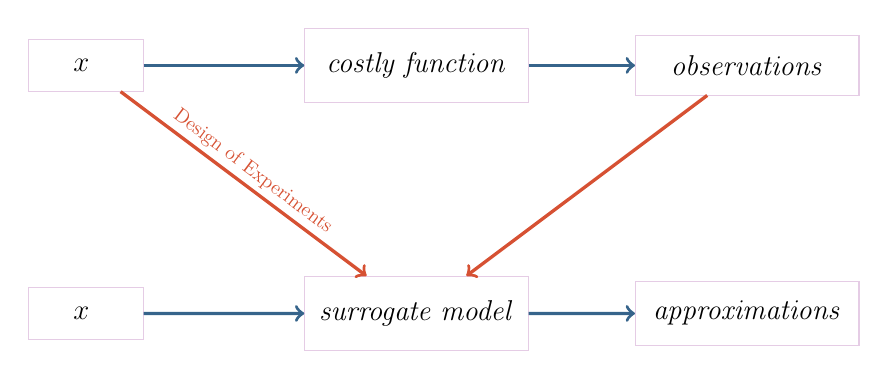
\begin{tikzpicture}[scale=0.7, every node/.style={scale=0.6}]

      % \tikzstyle{Sim}=[rectangle, draw=MonBleu!20, fill=MonBleu!0];
      % \tikzstyle{Meta}=[rectangle, draw=Orange!40, fill=MonBleu!0];
      \tikzstyle{Mes}=[rectangle, draw=violet!20, fill=violet!0];

        \node[Mes](MesIn) at (-6, 0) {
          \parbox{2.2cm}{ %
            \centering
            \LARGE
            \vspace{3mm}
            $x$
            \vspace{3mm}
          }};

        \node[Mes](Mes) at (0, 0) {
          \parbox{4.5cm}{ %
            \centering
            \LARGE
            \vspace{4mm}
            \textit{costly function}\\
            \vspace{4mm}
          }};

        \node[Mes](MesOut) at (6, 0) {
        \parbox{4.5cm}{ %
            \centering
            \LARGE
            \vspace{3mm}
          \textit{observations}\\
            \vspace{3mm}
        }};
        \draw[->, very thick, draw=MonBleu] (MesIn) -- (Mes.west);
        \draw[->, very thick, draw=MonBleu] (Mes) -- (MesOut.west);

        \node[Mes](MetaIn) at (-6, -4.5) {
          \parbox{2.2cm}{ %
          \centering
            \LARGE
            \vspace{3mm}
            $x$
            \vspace{3mm}
          }};

        \node[Mes](Meta) at (0, -4.5) {
          \parbox{4.5cm}{ %
            \centering
            \LARGE
            \vspace{4mm}
            \textit{surrogate model}\\
            \vspace{4mm}
          }};

        \node[Mes](MetaOut) at (6.0, -4.5) {
        \parbox{4.5cm}{ %
            \centering
            \LARGE
            \vspace{3mm}
          \textit{approximations}\\
            \vspace{3mm}
        }};

        \draw[->, very thick, draw=MonBleu] (MetaIn) -- (Meta.west);
        \draw[->, very thick, draw=MonBleu] (Meta) -- (MetaOut.west);

        \draw[->, very thick, draw=Orange!80] (MesIn) -- (Meta)
        node [above, midway, sloped, Orange!80] {\large Design of Experiments};
        \draw[->, very thick, draw=Orange!80] (MesOut)  -- (Meta);
        %node [above, midway, sloped, Orange!80] {\large réponses};

    \end{tikzpicture}
    \end{figure}
In practice, it is risky to take decisions based only on the model...\\
\vspace{3mm}
On the other hand, the model can be used to guide us in the search for the optimum.
\end{frame}

%%%%%%%%%%%%%%%%%%%%%%%%%%%%%%%%%%%%%%%%%%%%%%%%%%%%%%
\begin{frame}{}
\textbf{Global optimization} methods are a trade-off between
\begin{itemize}
	\item Exploitation of past good results
	\item Exploration of the space
\end{itemize}
\vspace{3mm}
\begin{center}
\textbf{How can GPR models be helpful?}\\
\includegraphics[height=5cm]{4_optimization/figures/python/ego_0}
\end{center}
\end{frame}

%%%%%%%%%%%%%%%%%%%%%%%%%%%%%%%%%%%%%%%%%%%%%%%%%%%%%%
\begin{frame}{}
In our example, the best observed value is 1.79
\begin{center}
\includegraphics[height=5cm]{4_optimization/figures/python/ego_improv}
\end{center}
Various criteria can be studied
\begin{itemize}
	\item probability of improvement
	\item Expected improvement
\end{itemize}
\end{frame}

%%%%%%%%%%%%%%%%%%%%%%%%%%%%%%%%%%%%%%%%%%%%%%%%%%%%%%
\begin{frame}{}
\textbf{Probability of Improvement:}
$$PI(x) = cdf \left(\frac{\min(F) - m(x)}{\sqrt{(c(x,x))}} \right)$$
\begin{center}
\includegraphics[height=5cm]{4_optimization/figures/python/ego_PI}
\end{center}
\end{frame}

%%%%%%%%%%%%%%%%%%%%%%%%%%%%%%%%%%%%%%%%%%%%%%%%%%%%%%
\begin{frame}{}
The point with the highest PI is often very close to the best observed value. We can show that there is a $x$ in the neighbourhood of $x^*$ such that $PI(x) \geq 0.5$.\\
\vspace{5mm}
For such points, the improvement cannot be large... \\
\vspace{3mm}
Can we find another criterion?
\end{frame}

%%%%%%%%%%%%%%%%%%%%%%%%%%%%%%%%%%%%%%%%%%%%%%%%%%%%%%
\begin{frame}{}
\textbf{Expected Improvement:}
\begin{equation*}
\begin{split}
E&I(x) =  \int_{-\infty}^{\min(F)} \max\left(0,Y(x)\right) ~dY(x) = \dots = \\
& \sqrt{c(x,x)} (u(x) cdf(u(x)) + pdf(u(x))) \quad \text{ with } u(x) = \frac{\min(F) - m(x)}{\sqrt{(c(x,x))}}
\end{split}
\end{equation*}
%\qquad with $ \displaystyle u(x) = \frac{\min(F) - m(x)}{\sqrt{(c(x,x))}}$
\begin{center}
\includegraphics[height=5cm]{4_optimization/figures/python/ego_EI0}
\end{center}
\end{frame}

%%%%%%%%%%%%%%%%%%%%%%%%%%%%%%%%%%%%%%%%%%%%%%%%%%%%%%
\begin{frame}{Expected Improvement}
Let's see how it works... iteration 1
\begin{center}
\includegraphics[height=5cm]{4_optimization/figures/python/ego_EI1}
\end{center}
\end{frame}

%%%%%%%%%%%%%%%%%%%%%%%%%%%%%%%%%%%%%%%%%%%%%%%%%%%%%%
\begin{frame}[noframenumbering]{Expected Improvement}
Let's see how it works... iteration 2
\begin{center}
\includegraphics[height=5cm]{4_optimization/figures/python/ego_EI2}
\end{center}
\end{frame}

%%%%%%%%%%%%%%%%%%%%%%%%%%%%%%%%%%%%%%%%%%%%%%%%%%%%%%
\begin{frame}[noframenumbering]{Expected Improvement}
Let's see how it works... iteration 3
\begin{center}
\includegraphics[height=5cm]{4_optimization/figures/python/ego_EI3}
\end{center}
\end{frame}

%%%%%%%%%%%%%%%%%%%%%%%%%%%%%%%%%%%%%%%%%%%%%%%%%%%%%%
\begin{frame}[noframenumbering]{Expected Improvement}
Let's see how it works... iteration 4
\begin{center}
\includegraphics[height=5cm]{4_optimization/figures/python/ego_EI4}
\end{center}
\end{frame}

%%%%%%%%%%%%%%%%%%%%%%%%%%%%%%%%%%%%%%%%%%%%%%%%%%%%%%
\begin{frame}[noframenumbering]{Expected Improvement}
Let's see how it works... iteration 5
\begin{center}
\includegraphics[height=5cm]{4_optimization/figures/python/ego_EI9}
\end{center}
\end{frame}

%%%%%%%%%%%%%%%%%%%%%%%%%%%%%%%%%%%%%%%%%%%%%%%%%%%%%%
\begin{frame}{Expected Improvement}
This algorithm is called \textbf{Efficient Global Optimization} (EGO, Jones et al., 1998):
\begin{enumerate}
	\item make an initial design of experiments $X$ and calculate the associated $F$, $t = \mathtt{length}(F)$
	\item built a GP from $(X,F)$ (max. log-likelihood on $\sigma$ and $\theta_i$'s)
	\item $X_{t+1}= \arg \max_x EI(x)$
	\item calculate $F_{t+1}=f(X_{t+1})$, increment $t$
	\item stop ($t>t^\text{max}$) or go to {\color{blue}2.}
\end{enumerate}
\vspace{5mm}
\begin{itemize}
	\item[+] EGO provides a good trade-off between exploitation and exploration without arbitrary parameters.
	\item[+] It requires few function observations (10 in the example) to get close to optimal regions.
\end{itemize}
%\begin{example}
%From the previous 5 iterations, we obtain $1.44e39$ for the conditioning of the covariance matrix. Eigenvalues are
%$$ (67.70,\  24.86,\  5.13,\  1.68,\  0.45,\  0.16,\  0.01,\  0.00,\  0.00,\ 0.00) $$
%\end{example}
\end{frame}

%%%%%%%%%%%%%%%%%%%%%%%%%%%%%%%%%%%%%%%%%%%%%%%%%%%%%%
\begin{frame}{}
\begin{exampleblock}{Illustration for $d=6$ (Hartman)}
	Illustration in higher dimension
\begin{center}
\includegraphics[height=5.5cm]{4_optimization/figures/egoHartman} \includegraphics[height=5.5cm]{4_optimization/figures/egoHartman2}
\end{center}
\small Source: \textit{DiceOptim}, Roustant, Ginsbourger and Deville, 2009.
\end{exampleblock}
\end{frame}

%%%%%%%%%%%%%%%%%%%%%%%%%%%%%%%%%%%%%%%%%%%%%%%%%%%%%%
\begin{frame}{}
\begin{exampleblock}{Example: surface displacements misfit minimization}
$\Rightarrow$ demo with \texttt{mainInversionPunctualDisplSource.R}\\
!!! normalize the data: WLS has a few very large values, it is always $>0$: make it more gaussian, 
$\mathtt{wls}\_norm = \log(1+\mathtt{wls})$ and all $x$'s and $\mathtt{wls}\_norm$ between 0 and 1.
\begin{minipage}[c]{0.6\textwidth}
\begin{center}
\includegraphics[width=\textwidth]{4_optimization/figures/misfit_learn_set} 
\end{center}
\end{minipage}
\hspace{0.3cm}
\begin{minipage}[c]{0.30\textwidth}
{\small 100 $\{xs,ys,zs,a,p\}$ points chosen through an optimized Latin Hypercube Sampling 
(\texttt{R} libraries \texttt{DiceDesign} or \texttt{lhs}).}\\
\end{minipage}
\end{exampleblock}
\end{frame}

%%%%%%%%%%%%%%%%%%%%%%%%%%%%%%%%%%%%%%%%%%%%%%%%%%%%%%
\begin{frame}{}
\small (demo with \texttt{mainInversionPunctualDisplSource.R}, cont.)
\begin{center}
\includegraphics[width=0.7\textwidth]{4_optimization/figures/misfit_test_set} 
\end{center}
{\tiny 110 random $\{xs,ys,zs,a,p\}$ test points.}\\
\end{frame}

%%%%%%%%%%%%%%%%%%%%%%%%%%%%%%%%%%%%%%%%%%%%%%%%%%%%%%
\begin{frame}{}
\small (demo with \texttt{mainInversionPunctualDisplSource.R}, cont.)
\begin{center}
\includegraphics[width=0.9\textwidth]{4_optimization/figures/misfit_test_set_2} 
\end{center}
{\tiny 110 test points.}\\
\end{frame}

%%%%%%%%%%%%%%%%%%%%%%%%%%%%%%%%%%%%%%%%%%%%%%%%%%%%%%
\begin{frame}{}
\small (demo with \texttt{mainInversionPunctualDisplSource.R}, cont.)\\
\small EGO parameters: anisotropic Mat\`ern 5/2 kernel, GP updated (log-likelihood maximized) every 5 added points, BFGS with bounded variables (from \texttt{optim()} function) restarted from random initial points for maximizing log-likelihood and EI.
\begin{minipage}[c]{0.6\textwidth}
\begin{center}
\includegraphics[width=\textwidth]{4_optimization/figures/misfit_EGO_conv} 
\end{center}
\end{minipage}
\hspace{0.3cm}
\begin{minipage}[c]{0.3\textwidth}
Preferential sampling of good regions of $S$, but global therefore sometimes increasing WLS.
\end{minipage}
\end{frame}

%%%%%%%%%%%%%%%%%%%%%%%%%%%%%%%%%%%%%%%%%%%%%%%%%%%%%%
\begin{frame}{}
\small (demo with \texttt{mainInversionPunctualDisplSource.R}, cont.)
\end{frame}

%%%%%%%%%%%%%%%%%%%%%%%%%%%%%%%%%%%%%%%%%%%%%%%%%%%%%%
\begin{frame}{}
\begin{exampleblock}{Difficulties and challenges with EGO}
\begin{itemize}
\item Standard GPs are limited to $n \approx 1000$ points (covariance matrix inversion).
\item EGO clusters points in good regions, the covariance matrix may become ill-conditionned 
if length scales $\theta_i$ are too small.
\item Although the method perfectly applies to large dimensional spaces ($d>100$), larger $d$ 
may require larger $n$, back 2 lines above.
\item EGO does not converge in the traditional sense: it creates dense samples in the volume of $S$. 
The efficiency comes from the order in which points are sampled.
\end{itemize}
$\Rightarrow$ these are the topics of current research. Let's mention a few extensions next.
\end{exampleblock}
\end{frame}

%%%%%%%%%%%%%%%%%%%%%%%%%%%%%%%%%%%%%%%%%%%%%%%%%%%%%%
\begin{frame}{}
One way to improve the conditioning of the covariance matrix is to replace two values that are close-by by one function value and one derivative:
\begin{center}
  \begin{tabular}{ccc}
\includegraphics[height=4cm]{4_optimization/figures/python/osborn0} &
\includegraphics[height=4cm]{4_optimization/figures/Rightarrow} &
\includegraphics[height=4cm]{4_optimization/figures/python/osborn1} \\
Cond. = 3842 & & Cond. = 10
  \end{tabular}
\end{center}
This can be generalised to higher orders \alert{$\rightarrow$} Taylor expansion\\
\small see articles from M. Osborn
\end{frame}

%%%%%%%%%%%%%%%%%%%%%%%%%%%%%%%%%%%%%%%%%%%%%%%%%%%%%%
\begin{frame}{}
If we know the computational budget in advance, adding new points at the \textbf{best one step ahead location} is not optimal.\\
\vspace{5mm}
Some improvements have been made toward this
\begin{itemize}
	\item Batch EGO
	\item Parallelization of the algorithm
\end{itemize}
\vspace{5mm}
\small see works from D. Ginsbourger
\end{frame}

%%%%%%%%%%%%%%%%%%%%%%%%%%%%%%%%%%%%%%%%%%%%%%%%%%%%%%
%%%%%%%%%%%%%%%%%%%%%%%%%%%%%%%%%%%%%%%%%%%%%%%%%%%%%%
\section[Robust optim.]{Robust optimization}
\subsection{}

%%%%%%%%%%%%%%%%%%%%%%%%%%%%%%%%%%%%%%%%%%%%%%%%%%%%%%
\begin{frame}{}
Robust optimization may mean various things:
\begin{itemize}
	\item There is observation noise on the output
	\item Some input variables are uncertain
	\item Model is uncertain
\end{itemize}
\vspace{2mm}
\begin{example}
\begin{columns}[c]
\column{3cm}
	\includegraphics[height=4cm]{4_optimization/figures/RLRrobust}
\column{5cm}
	a +/- 1mm dispersion in the manufacturing of a car cylinder head  can degrade its performance (g CO2/km) by -20\% (worst case)\\
\end{columns}
\vspace{3mm}
	\small Source: Talk from R. Le Riche at the Porquerolles Summer School, 2014
\end{example}
\end{frame}

%%%%%%%%%%%%%%%%%%%%%%%%%%%%%%%%%%%%%%%%%%%%%%%%%%%%%%
\begin{frame}{}
% \begin{example}
% Here is a basic example:
% \begin{center}
% \includegraphics[height=5cm]{4_optimization/figures/optim_rob_a}\\
% Which input is the best?
% \end{center}
% \end{example}
% \end{frame}

% %%%%%%%%%%%%%%%%%%%%%%%%%%%%%%%%%%%%%%%%%%%%%%%%%%%%%%
% \begin{frame}[noframenumbering]{}
\begin{example}
Here is a basic example:
\begin{center}
\includegraphics[height=5cm]{4_optimization/figures/optim_rob_b}\\
Which input is the best?
\end{center}
\end{example}
\end{frame}

%%%%%%%%%%%%%%%%%%%%%%%%%%%%%%%%%%%%%%%%%%%%%%%%%%%%%%
\begin{frame}[noframenumbering]{}
\begin{example}
A non Gaussian example
\begin{center}
\includegraphics[height=5cm]{4_optimization/figures/optim_rob_c}\\
In some cases, we may want to optimize the worst case scenario.
\end{center}
\end{example}
\end{frame}

%%%%%%%%%%%%%%%%%%%%%%%%%%%%%%%%%%%%%%%%%%%%%%%%%%%%%%
\begin{frame}{}
Can EGO be adapted when observations are noisy?\\
\vspace{5mm}
First of all, using the current best observation as a minimum does not make much sense...\\
\vspace{5mm}
Some solutions are
\begin{itemize}
	\item[S1] Build a new model that interpolates $m(X)$ at $X$.
	\item[S2] Include observation noise and replace $\min(F)$ by $\min(m(X))$ in the EI expression
	\item[S3] Similar to 2 but consider an Expected Mean Improvement.
\end{itemize}
\end{frame}

%%%%%%%%%%%%%%%%%%%%%%%%%%%%%%%%%%%%%%%%%%%%%%%%%%%%%%
\begin{frame}{Solution 1}
iteration 0
\begin{center}
\includegraphics[height=5cm]{4_optimization/figures/python/ego_EI1n0}
\end{center}
\end{frame}

%%%%%%%%%%%%%%%%%%%%%%%%%%%%%%%%%%%%%%%%%%%%%%%%%%%%%%
\begin{frame}[noframenumbering]{Solution 1}
iteration 1
\begin{center}
\includegraphics[height=5cm]{4_optimization/figures/python/ego_EI1n1}
\end{center}
\end{frame}

%%%%%%%%%%%%%%%%%%%%%%%%%%%%%%%%%%%%%%%%%%%%%%%%%%%%%%
\begin{frame}[noframenumbering]{Solution 1}
iteration 2
\begin{center}
\includegraphics[height=5cm]{4_optimization/figures/python/ego_EI1n2}
\end{center}
\end{frame}

%%%%%%%%%%%%%%%%%%%%%%%%%%%%%%%%%%%%%%%%%%%%%%%%%%%%%%
\begin{frame}[noframenumbering]{Solution 1}
iteration 3
\begin{center}
\includegraphics[height=5cm]{4_optimization/figures/python/ego_EI1n3}
\end{center}
\end{frame}

%%%%%%%%%%%%%%%%%%%%%%%%%%%%%%%%%%%%%%%%%%%%%%%%%%%%%%
\begin{frame}[noframenumbering]{Solution 1}
iteration 4
\begin{center}
\includegraphics[height=5cm]{4_optimization/figures/python/ego_EI1n4}
\end{center}
\end{frame}

%%%%%%%%%%%%%%%%%%%%%%%%%%%%%%%%%%%%%%%%%%%%%%%%%%%%%%
%%%%%%%%%%%%%%%%%%%%%%%%%%%%%%%%%%%%%%%%%%%%%%%%%%%%%%
\section[Related problems]{Related problems}
\subsection{}

%%%%%%%%%%%%%%%%%%%%%%%%%%%%%%%%%%%%%%%%%%%%%%%%%%%%%%
\begin{frame}{}
Some related optimization problems are:
\begin{itemize}
	\item calibration problems
	\item probability computations
\end{itemize}
\vspace{8mm}
Some algorithms with an EGO spirit can be applied:
\begin{itemize}
 	\item SUR methods
 \end{itemize}
\end{frame}

%%%%%%%%%%%%%%%%%%%%%%%%%%%%%%%%%%%%%%%%%%%%%%%%%%%%%%
\begin{frame}{}
We want to find the input(s) such that f(x) = 3.2
\begin{center}
\includegraphics[height=5cm]{4_optimization/figures/python/inv}
\end{center}
\end{frame}

%%%%%%%%%%%%%%%%%%%%%%%%%%%%%%%%%%%%%%%%%%%%%%%%%%%%%%
\begin{frame}[noframenumbering]{}
iteration 0:
\begin{center}
\includegraphics[height=5cm]{4_optimization/figures/python/invproba}
\end{center}
\end{frame}

%%%%%%%%%%%%%%%%%%%%%%%%%%%%%%%%%%%%%%%%%%%%%%%%%%%%%%
\begin{frame}[noframenumbering]{}
iteration 1:
\begin{center}
\includegraphics[height=5cm]{4_optimization/figures/python/invproba1}
\end{center}
\end{frame}

%%%%%%%%%%%%%%%%%%%%%%%%%%%%%%%%%%%%%%%%%%%%%%%%%%%%%%
\begin{frame}[noframenumbering]{}
iteration 2:
\begin{center}
\includegraphics[height=5cm]{4_optimization/figures/python/invproba2}
\end{center}
\end{frame}

%%%%%%%%%%%%%%%%%%%%%%%%%%%%%%%%%%%%%%%%%%%%%%%%%%%%%%
\begin{frame}[noframenumbering]{}
iteration 3:
\begin{center}
\includegraphics[height=5cm]{4_optimization/figures/python/invproba3}
\end{center}
\end{frame}


%%%%%%%%%%%%%%%%%%%%%%%%%%%%%%%%%%%%%%%%%%%%%%%%%%%%%%
%%%%%%%%%%%%%%%%%%%%%%%%%%%%%%%%%%%%%%%%%%%%%%%%%%%%%%
\section[Conclusions]{Concluding remarks}
\subsection{}
%%%%%%%%%%%%%%%%%%%%%%%%%%%%%%%%%%%%%%%%%%%%%%%%%%%%%%
\begin{frame}{}
\begin{exampleblock}{Conclusions}
\begin{itemize}
\item Gaussian Processes offer a mathematically funded and versatile framework for building statistical models.
\item The main assumptions are: the phenomenon output is Gaussian, functional choice of covariance function (kernel).
\item The statistical model needs physical knowledge: through data + expertise guiding the choice of kernel (which may come from the physical model).
\item The statistical model is in essence complementary to the physical model and typically useful 
for decision making (optimization, uncertainty propagation, \dots).
\end{itemize}
\end{exampleblock}

\end{frame}



\end{document}
